代码及相关数据文件已开源至\href{https://github.com/Word2VecT/Lianjia-Spider-Demo}{GitHub}。

\section{数据抓取}

使用 Scrapy 进行爬取,直接在数据爬取实验代码上改进而来。由于直接访问只能爬取到 100 页总共 3000 条数据,因此采用分类爬取的策略。首先不添加分类限制条件,判断总页数是否是 100,是则进行分类,分区域依次进行爬取,如果页数仍然是 100,则在分区域的基础上,分价格进行爬取,同理依次选择区域、价格、房型、朝向、楼高作为条件进行爬取。通过以上的限制条件分类爬取,实现了租房数据的全部获取。

同时链家具有反爬机制,短时间多次访问会被直接 302 重定向至验证码页面,我们采用了以下的反爬策略:\begin{itemize}
    \item 采用随机 User-Agent,模拟不同的浏览器访问。
    \item 采用\href{https://www.kuaidaili.com}{快代理}提供的隧道代理服务,并设置每次请求更换 IP,值得注意的是,由于已经采用代理,无需设置 cookie,设置后反而会被封。
    \item 采用延时策略,每次请求后延时 0.5 秒,避免短时间内多次访问。
    \item 设置检测重试机制,由于未设置 cookie,未登录状态下可能会有小程序弹窗,刷新后消失,因此设置中间件 middleware 当未检测到数据时,自动重试。
    \item 设置自定义重定向重试机制,由于某些代理 ip 可能因为多次访问被链家封禁,这个时候换个 ip 刷新即可正常访问,而 Scarpy 的默认重定向的重试机制是,跟随重定向页面后刷新重试,设置中间件 middleware,取消跟随,在原始页面重试。
    \item 为避免个性化推荐引起不同 ip 爬取内容重复,设置 \texttt{COOKIES\_ENABLED = False}。
\end{itemize}

\begin{python3code}
    def parse_city(self, response):
        """Parse the city-level rental homepage to determine if further subdivision is needed."""
        self.logger.info(f"Parsing city page: {response.url}")
        total_page = self.get_total_page(response) or 0
        total_count = self.get_total_count(response) or 0
        if total_page == 100 or total_count > 3000:
            area_half_url_list = response.xpath(
                '//div[@class="filter"]/div[@class="filter__wrapper w1150"]/ul[@data-target="area"]//li/a/@href'
            ).getall()
            area_half_url_list = [url for url in area_half_url_list if url != "/zufang/"]
            for area_half_url in area_half_url_list:
                area_url = f"{self.base_url}{area_half_url}"
                yield scrapy.Request(url=area_url, callback=self.parse_area, dont_filter=True)
        else:
            yield from self.to_parse(response.url, total_page, total_count)

    def parse_area(self, response):
        """Parse an area category to determine if further subdivision by price is needed."""
        self.logger.info(f"Parsing area page: {response.url}")
        total_page = self.get_total_page(response)
        total_count = self.get_total_count(response)
        if total_page == 100 or total_count > 3000:
            for i in range(1, self.max_price_page + 1):
                price_url = f"{response.url}rp{i}/"
                yield scrapy.Request(url=price_url, callback=self.parse_price, dont_filter=True)
        else:
            yield from self.to_parse(response.url, total_page, total_count)

    # 剩余同理
\end{python3code}

\section{数据处理}

整体数据采用 json 文件存储以保存层级信息,分析数据用 csv 文件存储,并采用 Data Wrangler 进行处理。

预处理时,首先判断是否存在数据,如果存在则进行数据清洗,进行去除无效字符和多余空白等操作,并设置缺省值。

\begin{python3code}
    # Extract description and clean it
    des = house.xpath(
        './div[@class="content__list--item--main"]/p[@class="content__list--item--des"]//text()'
    ).getall()
    item["des"] = ["".join(text.split()) for text in des if text.strip() and text.strip() not in ["-", "/"]]

    # Extract bottom info or set an empty list if None
    item["bottom"] = [
        text.strip()
        for text in house.xpath(
            './div[@class="content__list--item--main"]/p[@class="content__list--item--bottom oneline"]//i/text()'
        ).getall()
        if text.strip()
    ] or []

    # Extract brand or set a default value
    brand = house.xpath(
        './div[@class="content__list--item--main"]/p[@class="content__list--item--brand oneline"]/span[@class="brand"]/text()'
    ).get()
    item["brand"] = brand.strip() if brand else "N/A"

    # 其他同理
\end{python3code}

针对不同的任务,编写不同的 filter 脚本进一步处理数据,并保存至 csv 文件。

\section{数据分析}

\subsection{房租分析}
为了直观比较大小信息,采用直方图进行展示,同时为了更好地进行纬度比较,采用雷达图进行展示比较。

\subsubsection{租金对比}
见图~\ref{fig:price_bar_chart}、图~\ref{fig:price_radar_chart}。
\begin{figure}[htbp]
    \centering
    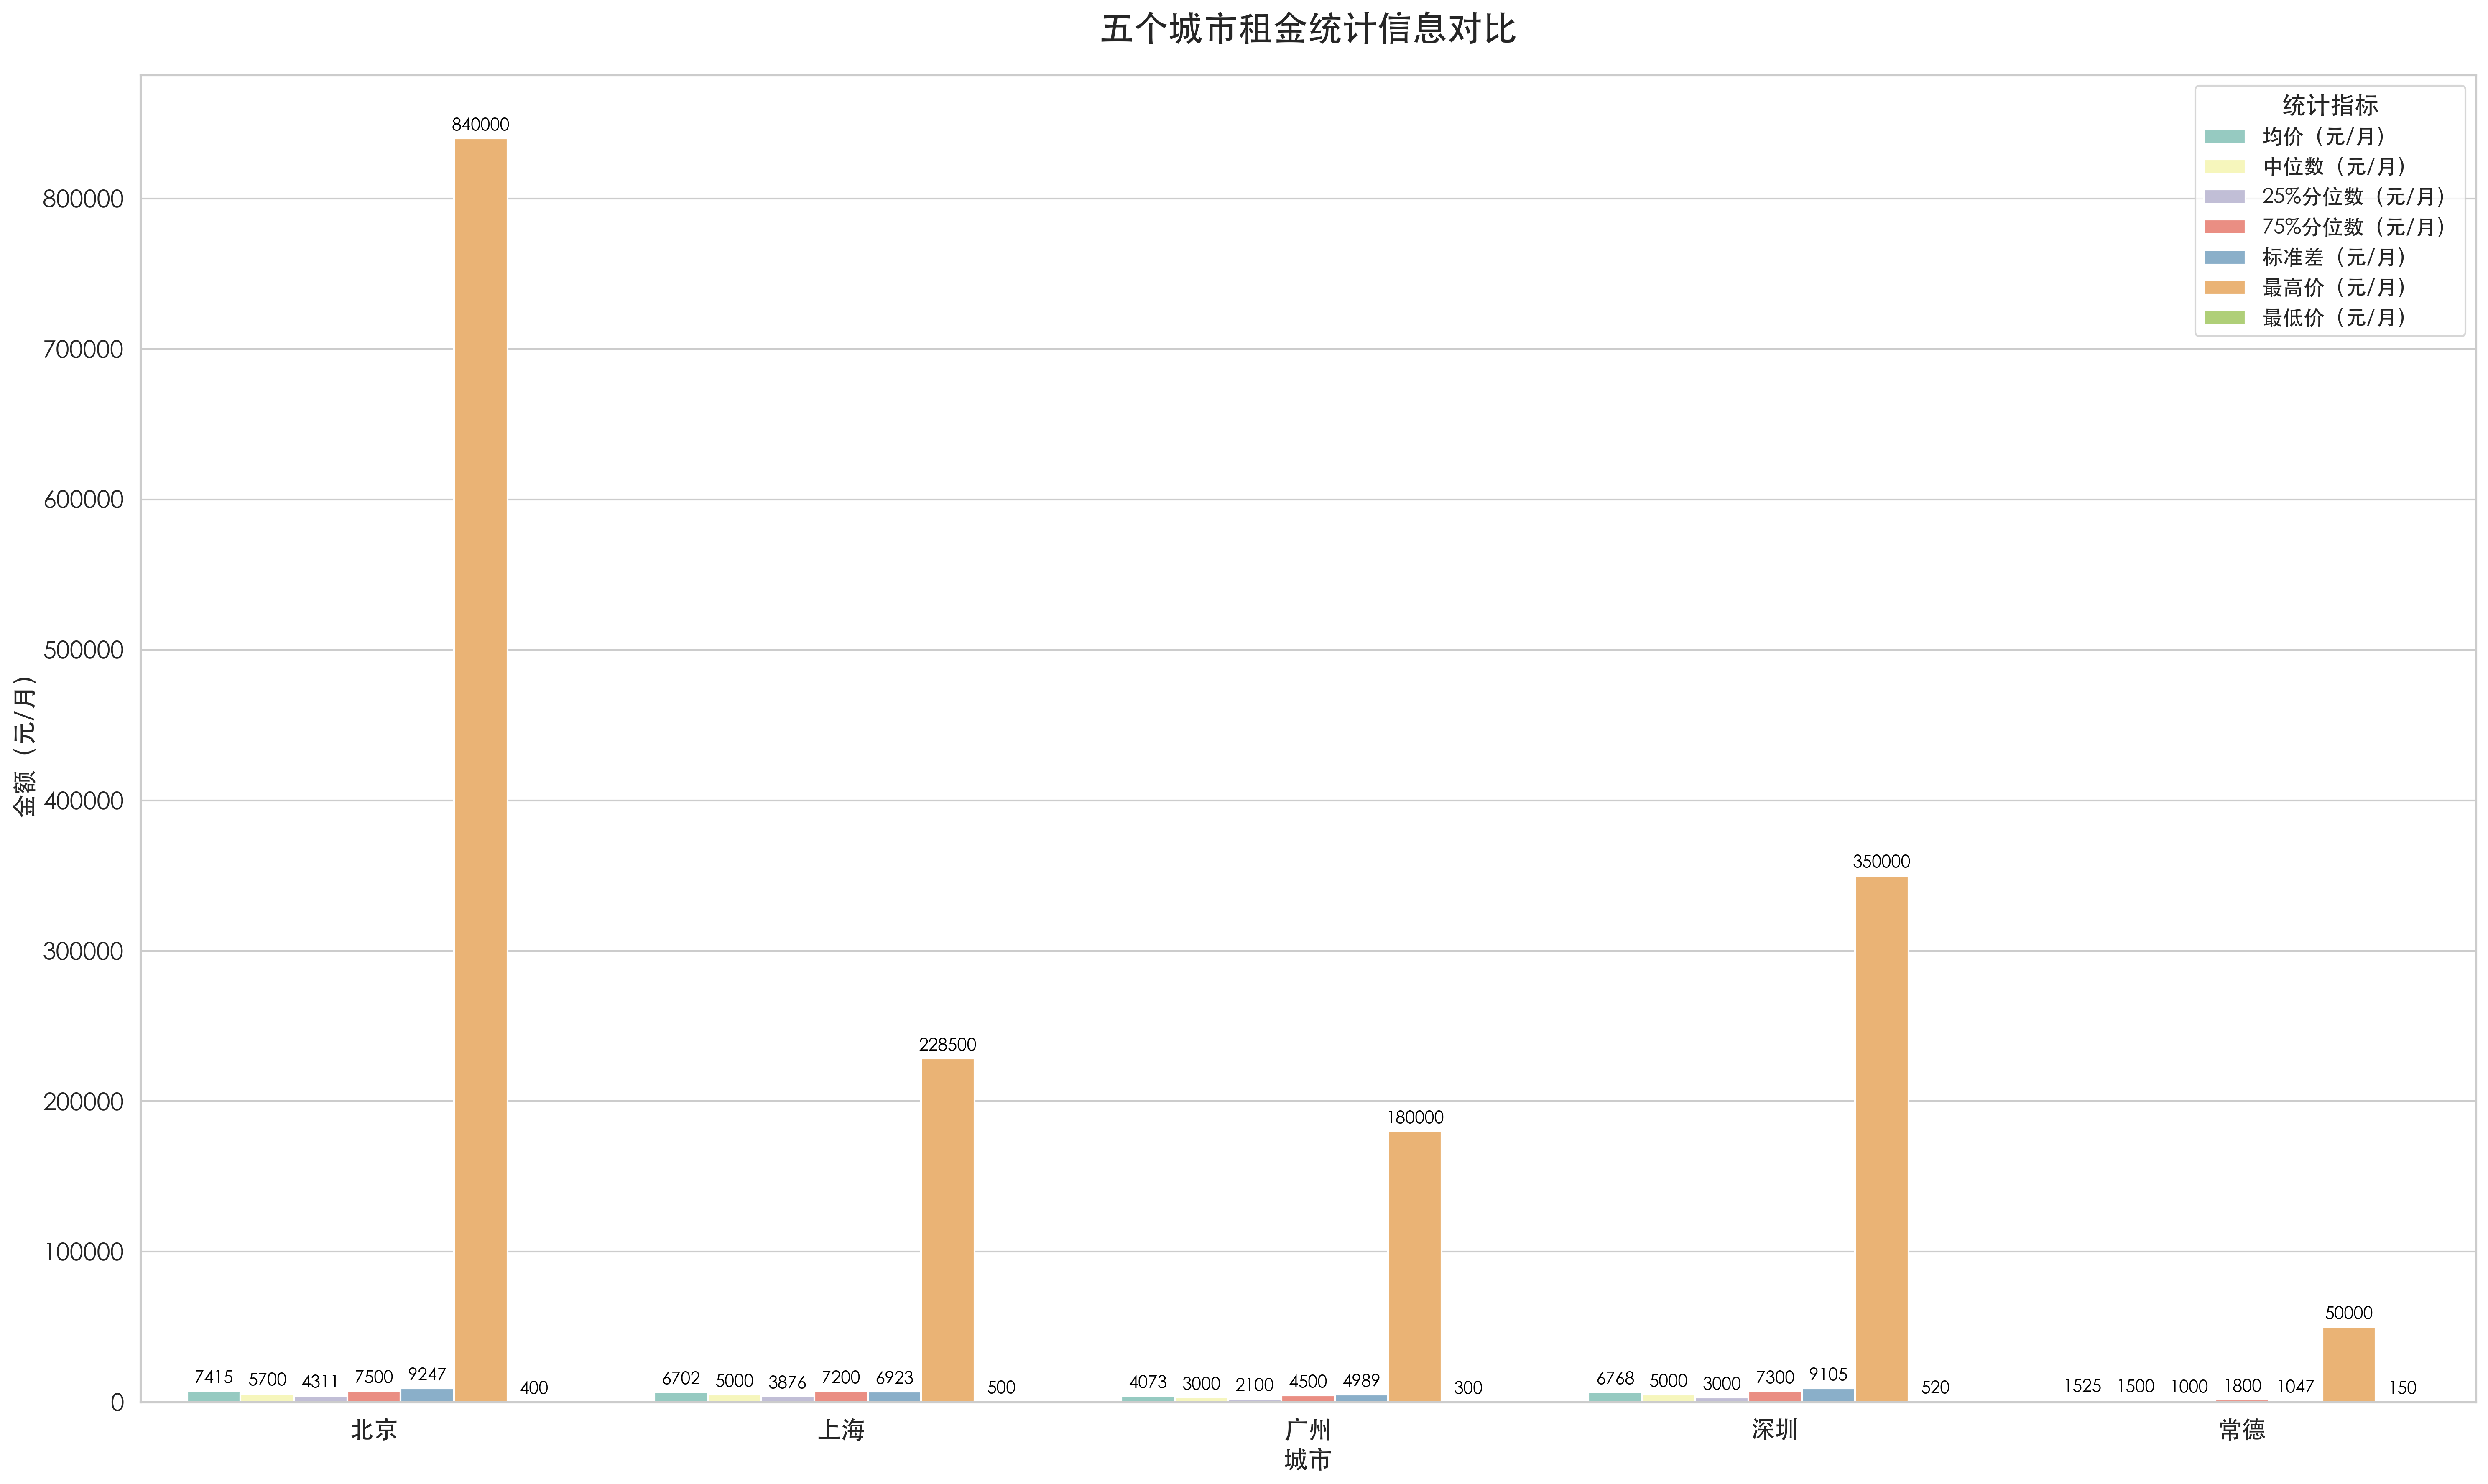
\includegraphics[width=0.7\linewidth]{../../figure/price_bar_chart.png}
    \caption{五个城市租金统计信息对比}
    \label{fig:price_bar_chart}
\end{figure}
\begin{figure}[htbp]
    \centering
    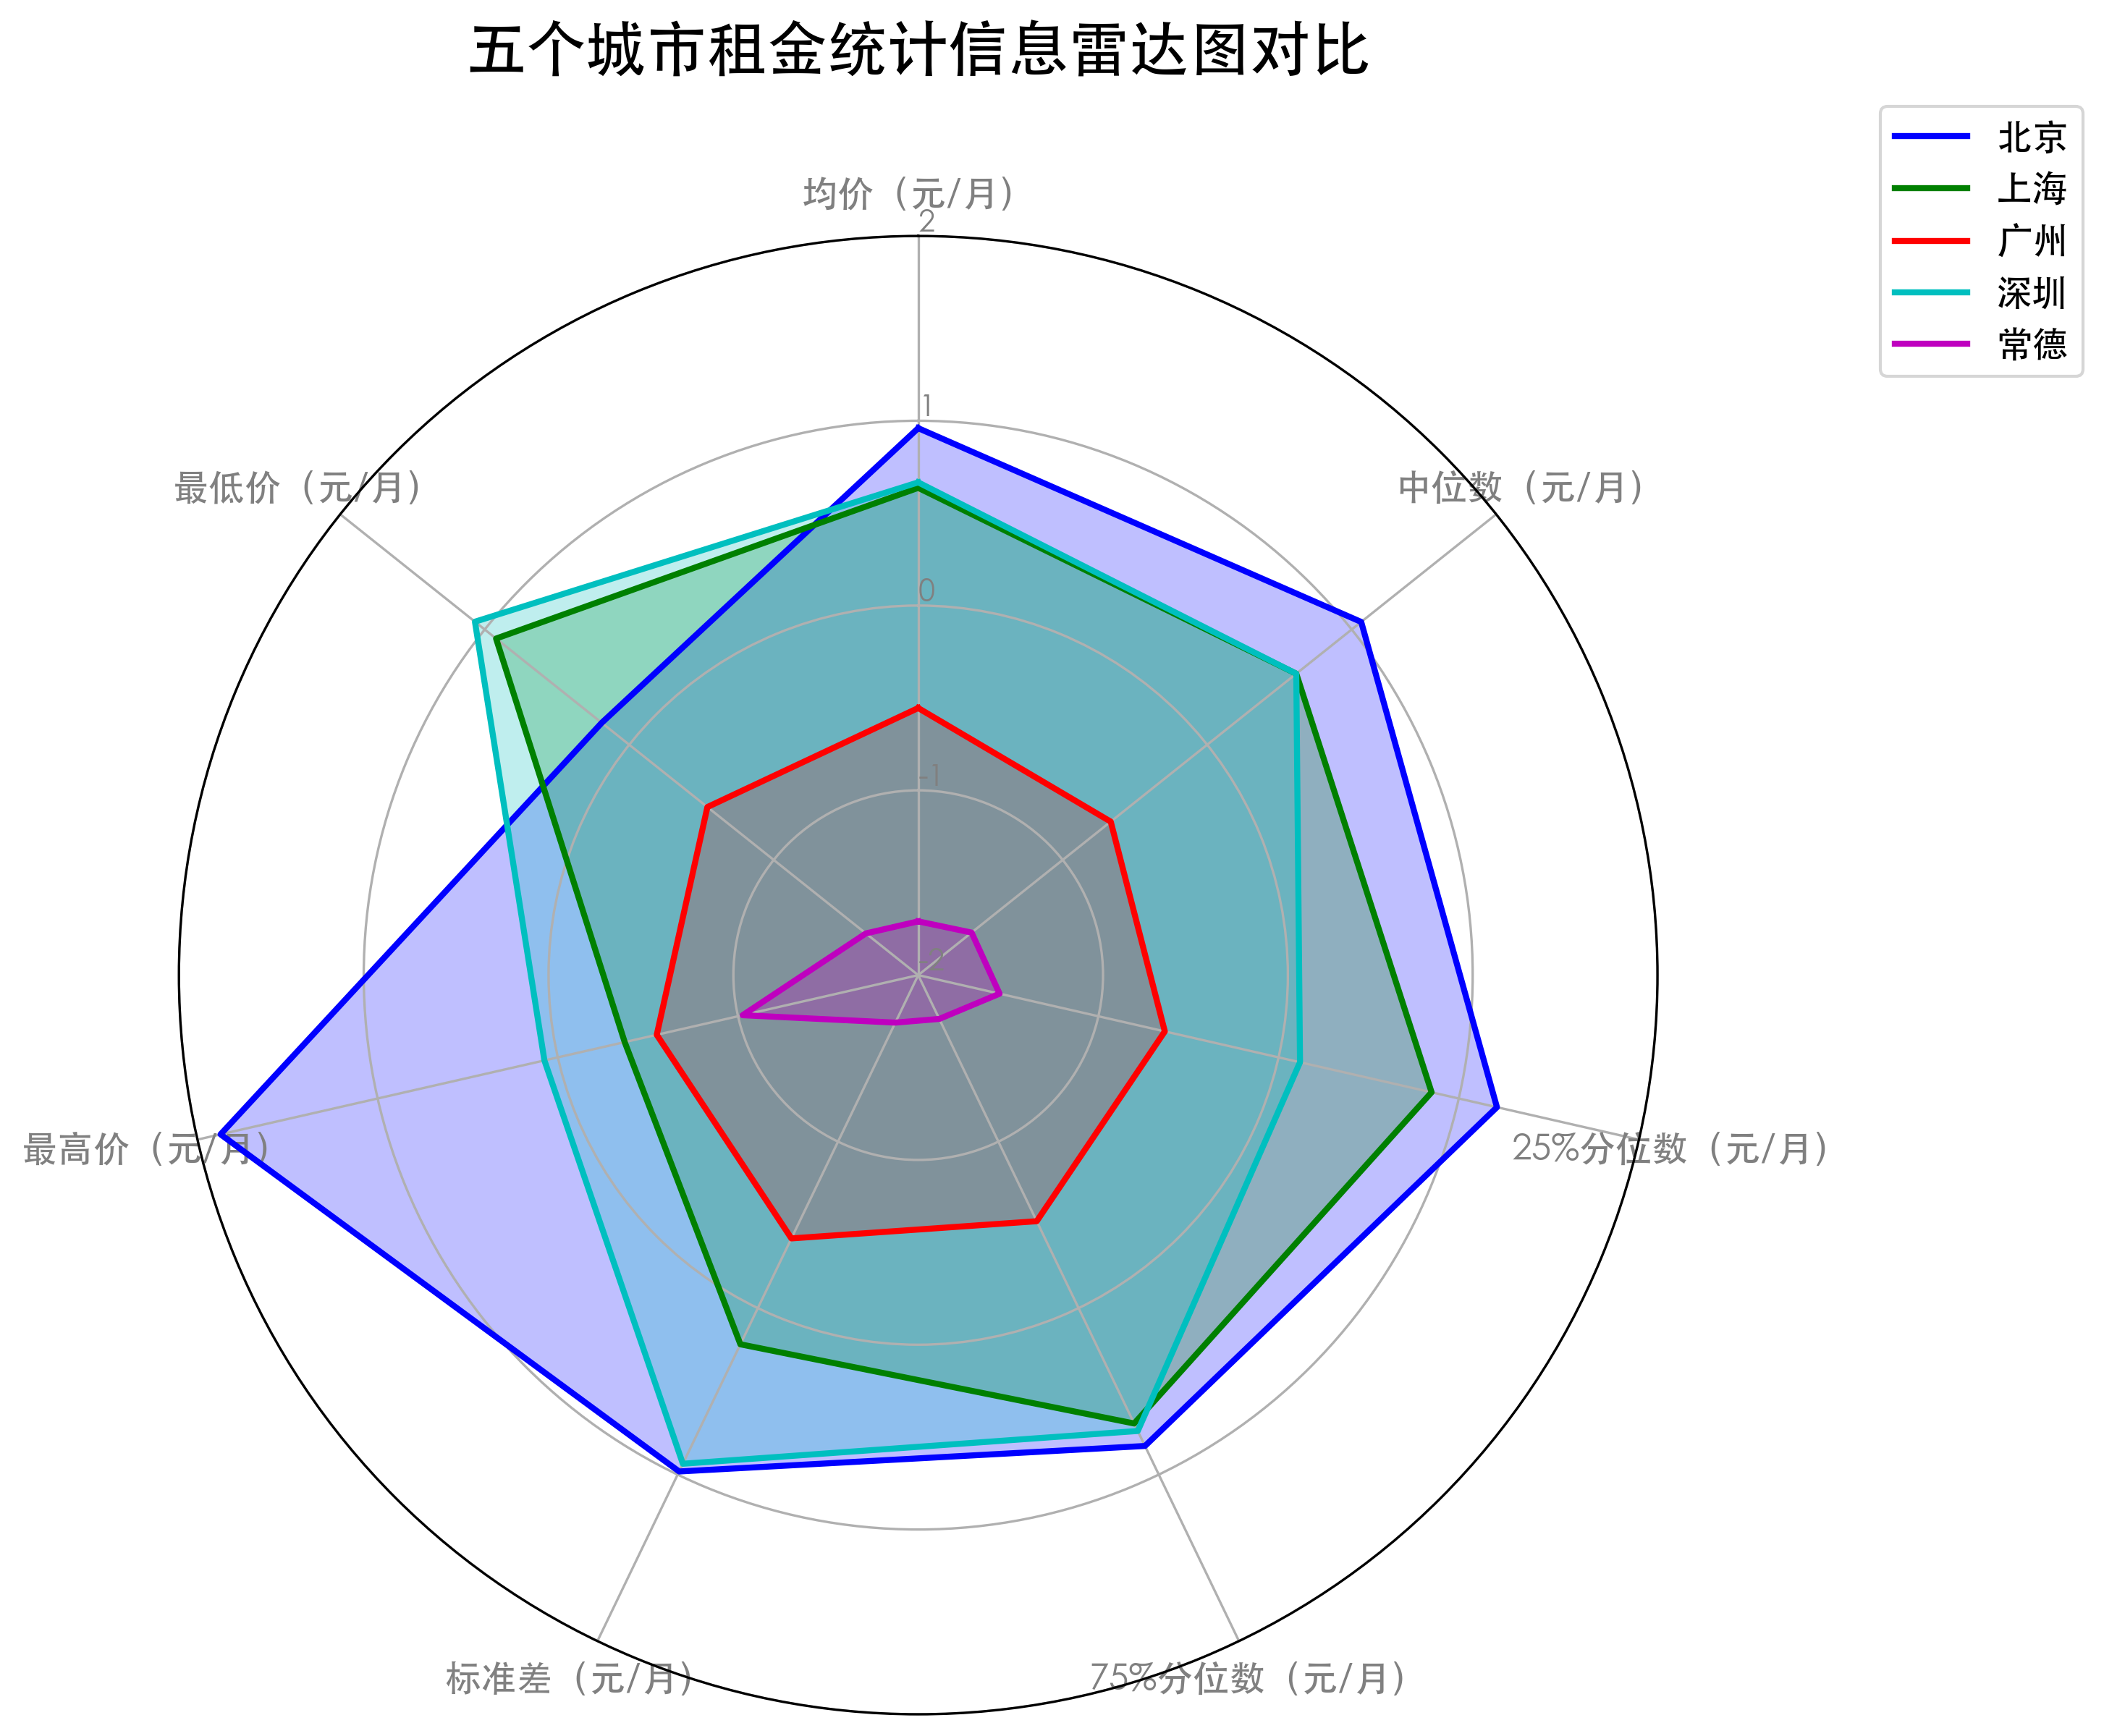
\includegraphics[width=0.7\linewidth]{../../figure/price_radar_chart.png}
    \caption{五个城市租金统计信息雷达图对比}
    \label{fig:price_radar_chart}
\end{figure}

\subsubsection{单位面积租金对比}
见图~\ref{fig:unit_price_bar_chart}、图~\ref{fig:unit_price_radar_chart}。
\begin{figure}[htbp]
    \centering
    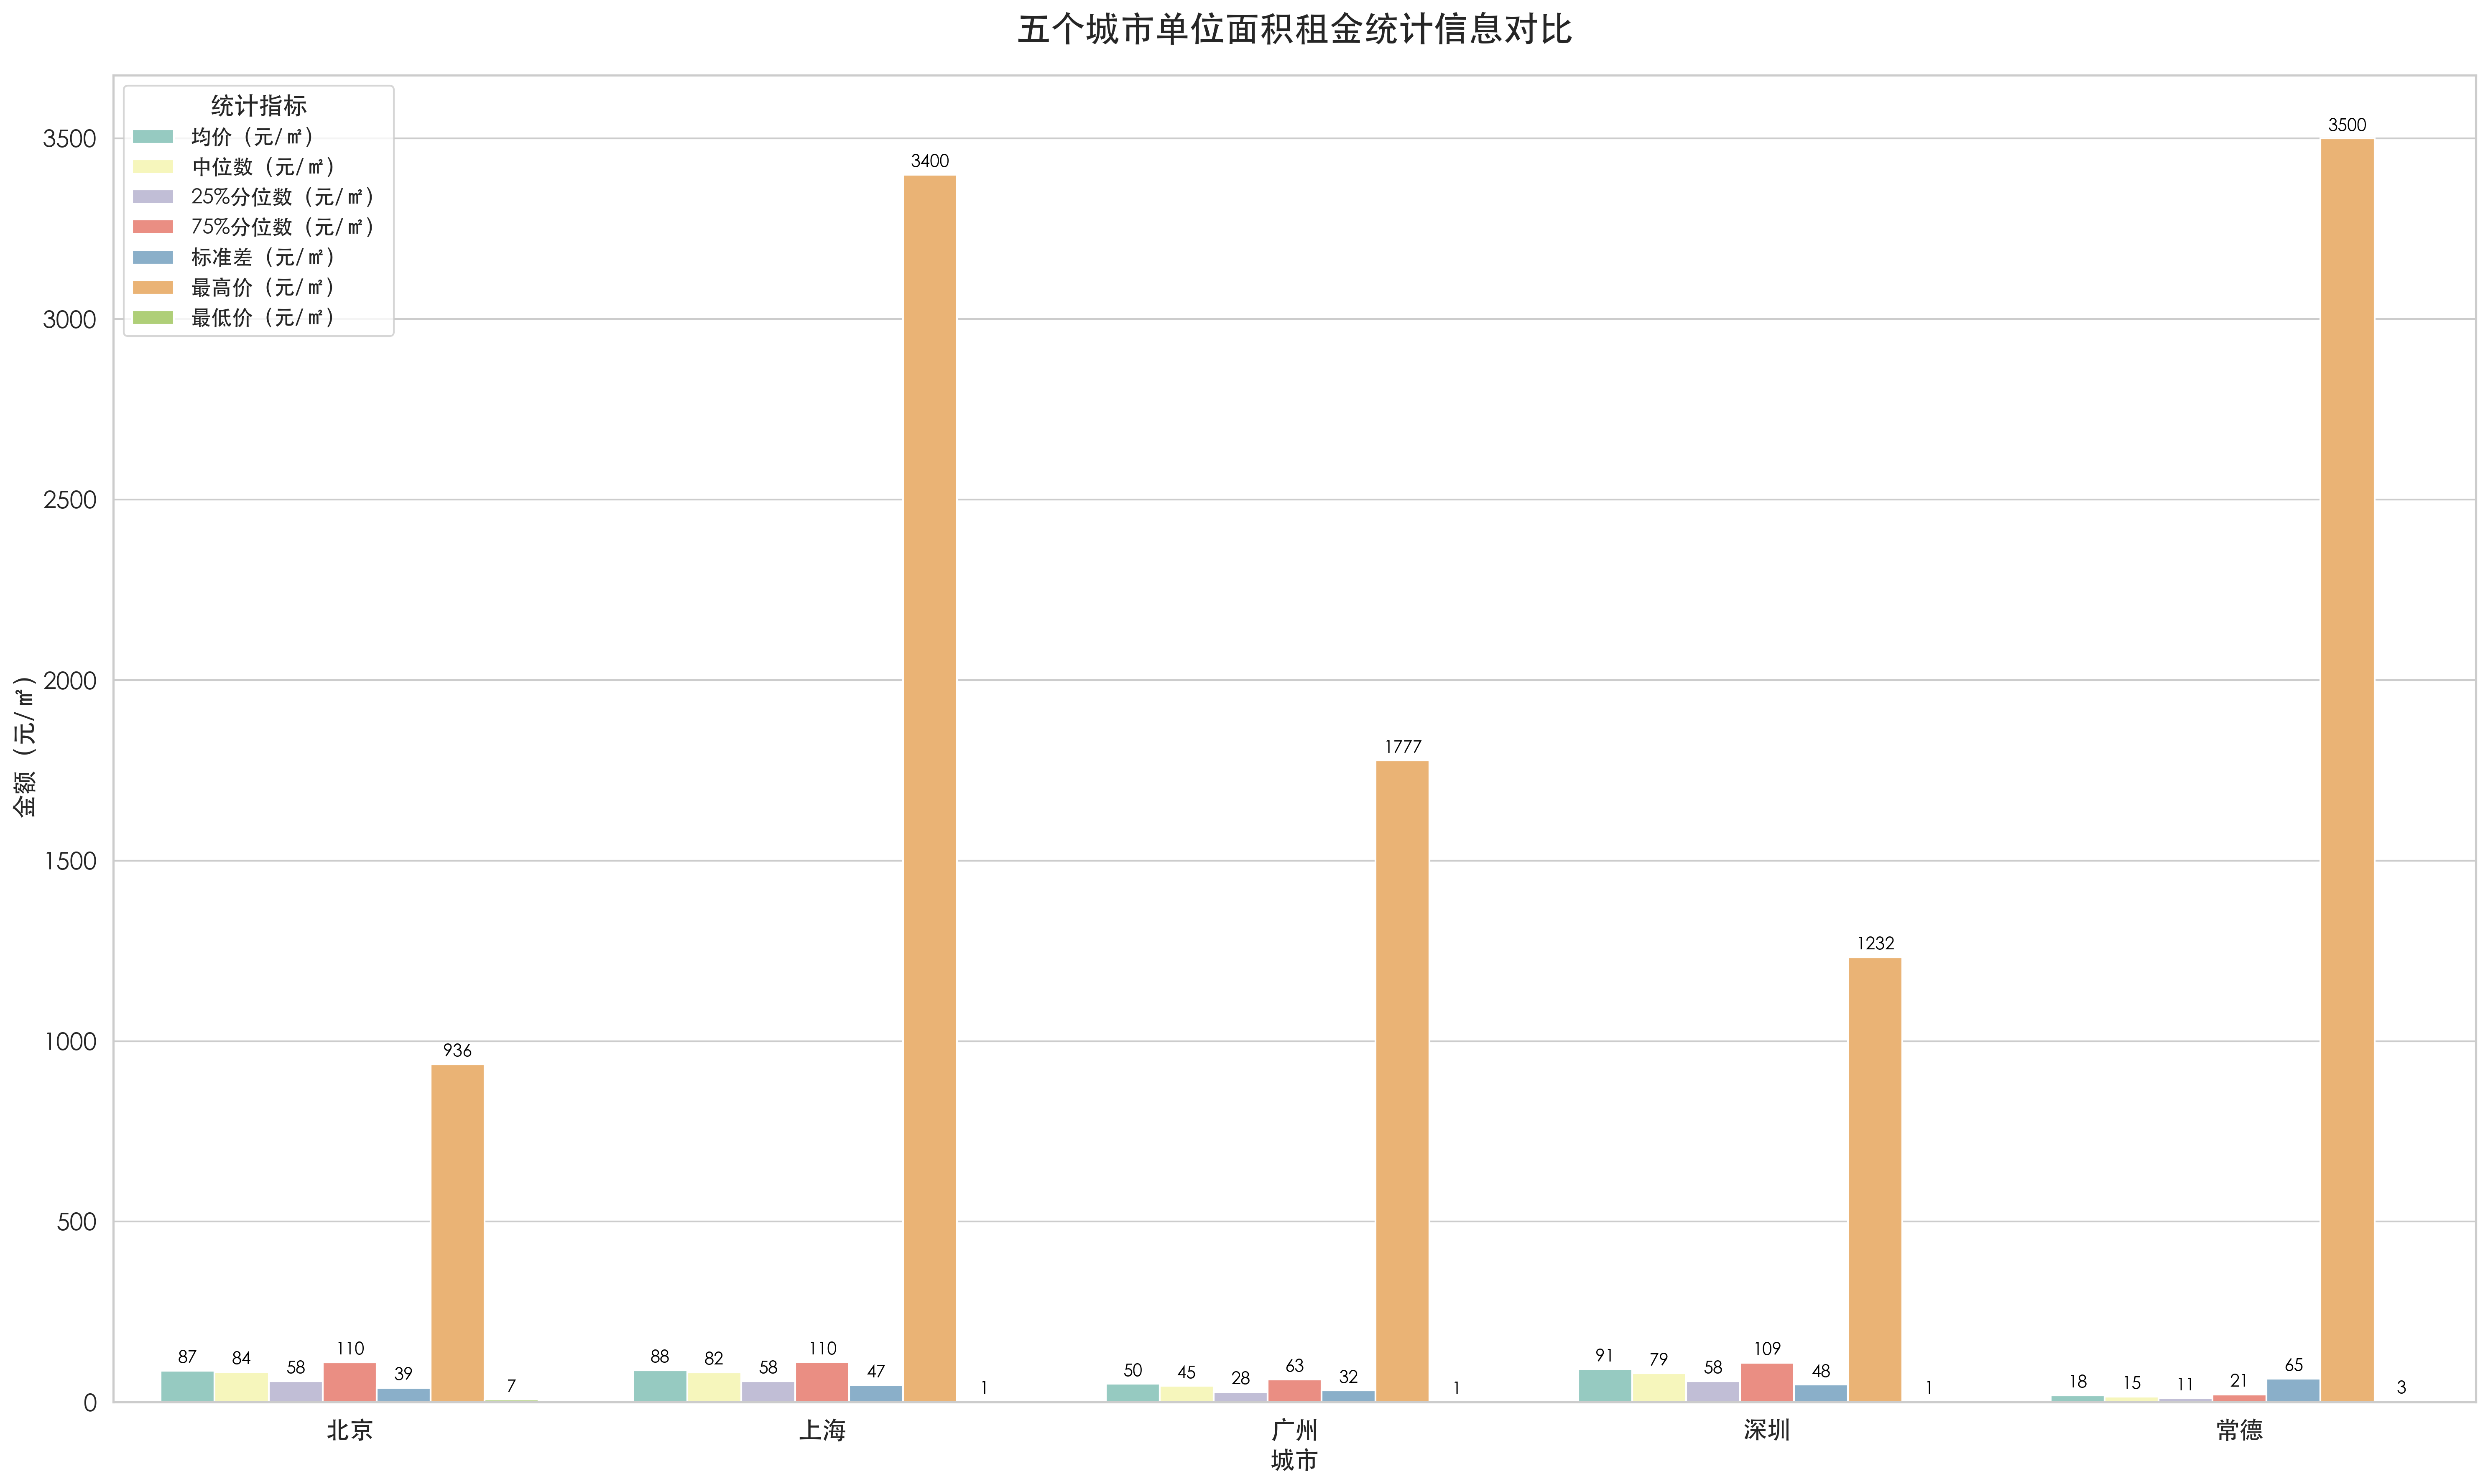
\includegraphics[width=0.7\linewidth]{../../figure/unit_price_bar_chart.png}
    \caption{五个城市单位面积租金统计信息对比}
    \label{fig:unit_price_bar_chart}
\end{figure}
\begin{figure}[htbp]
    \centering
    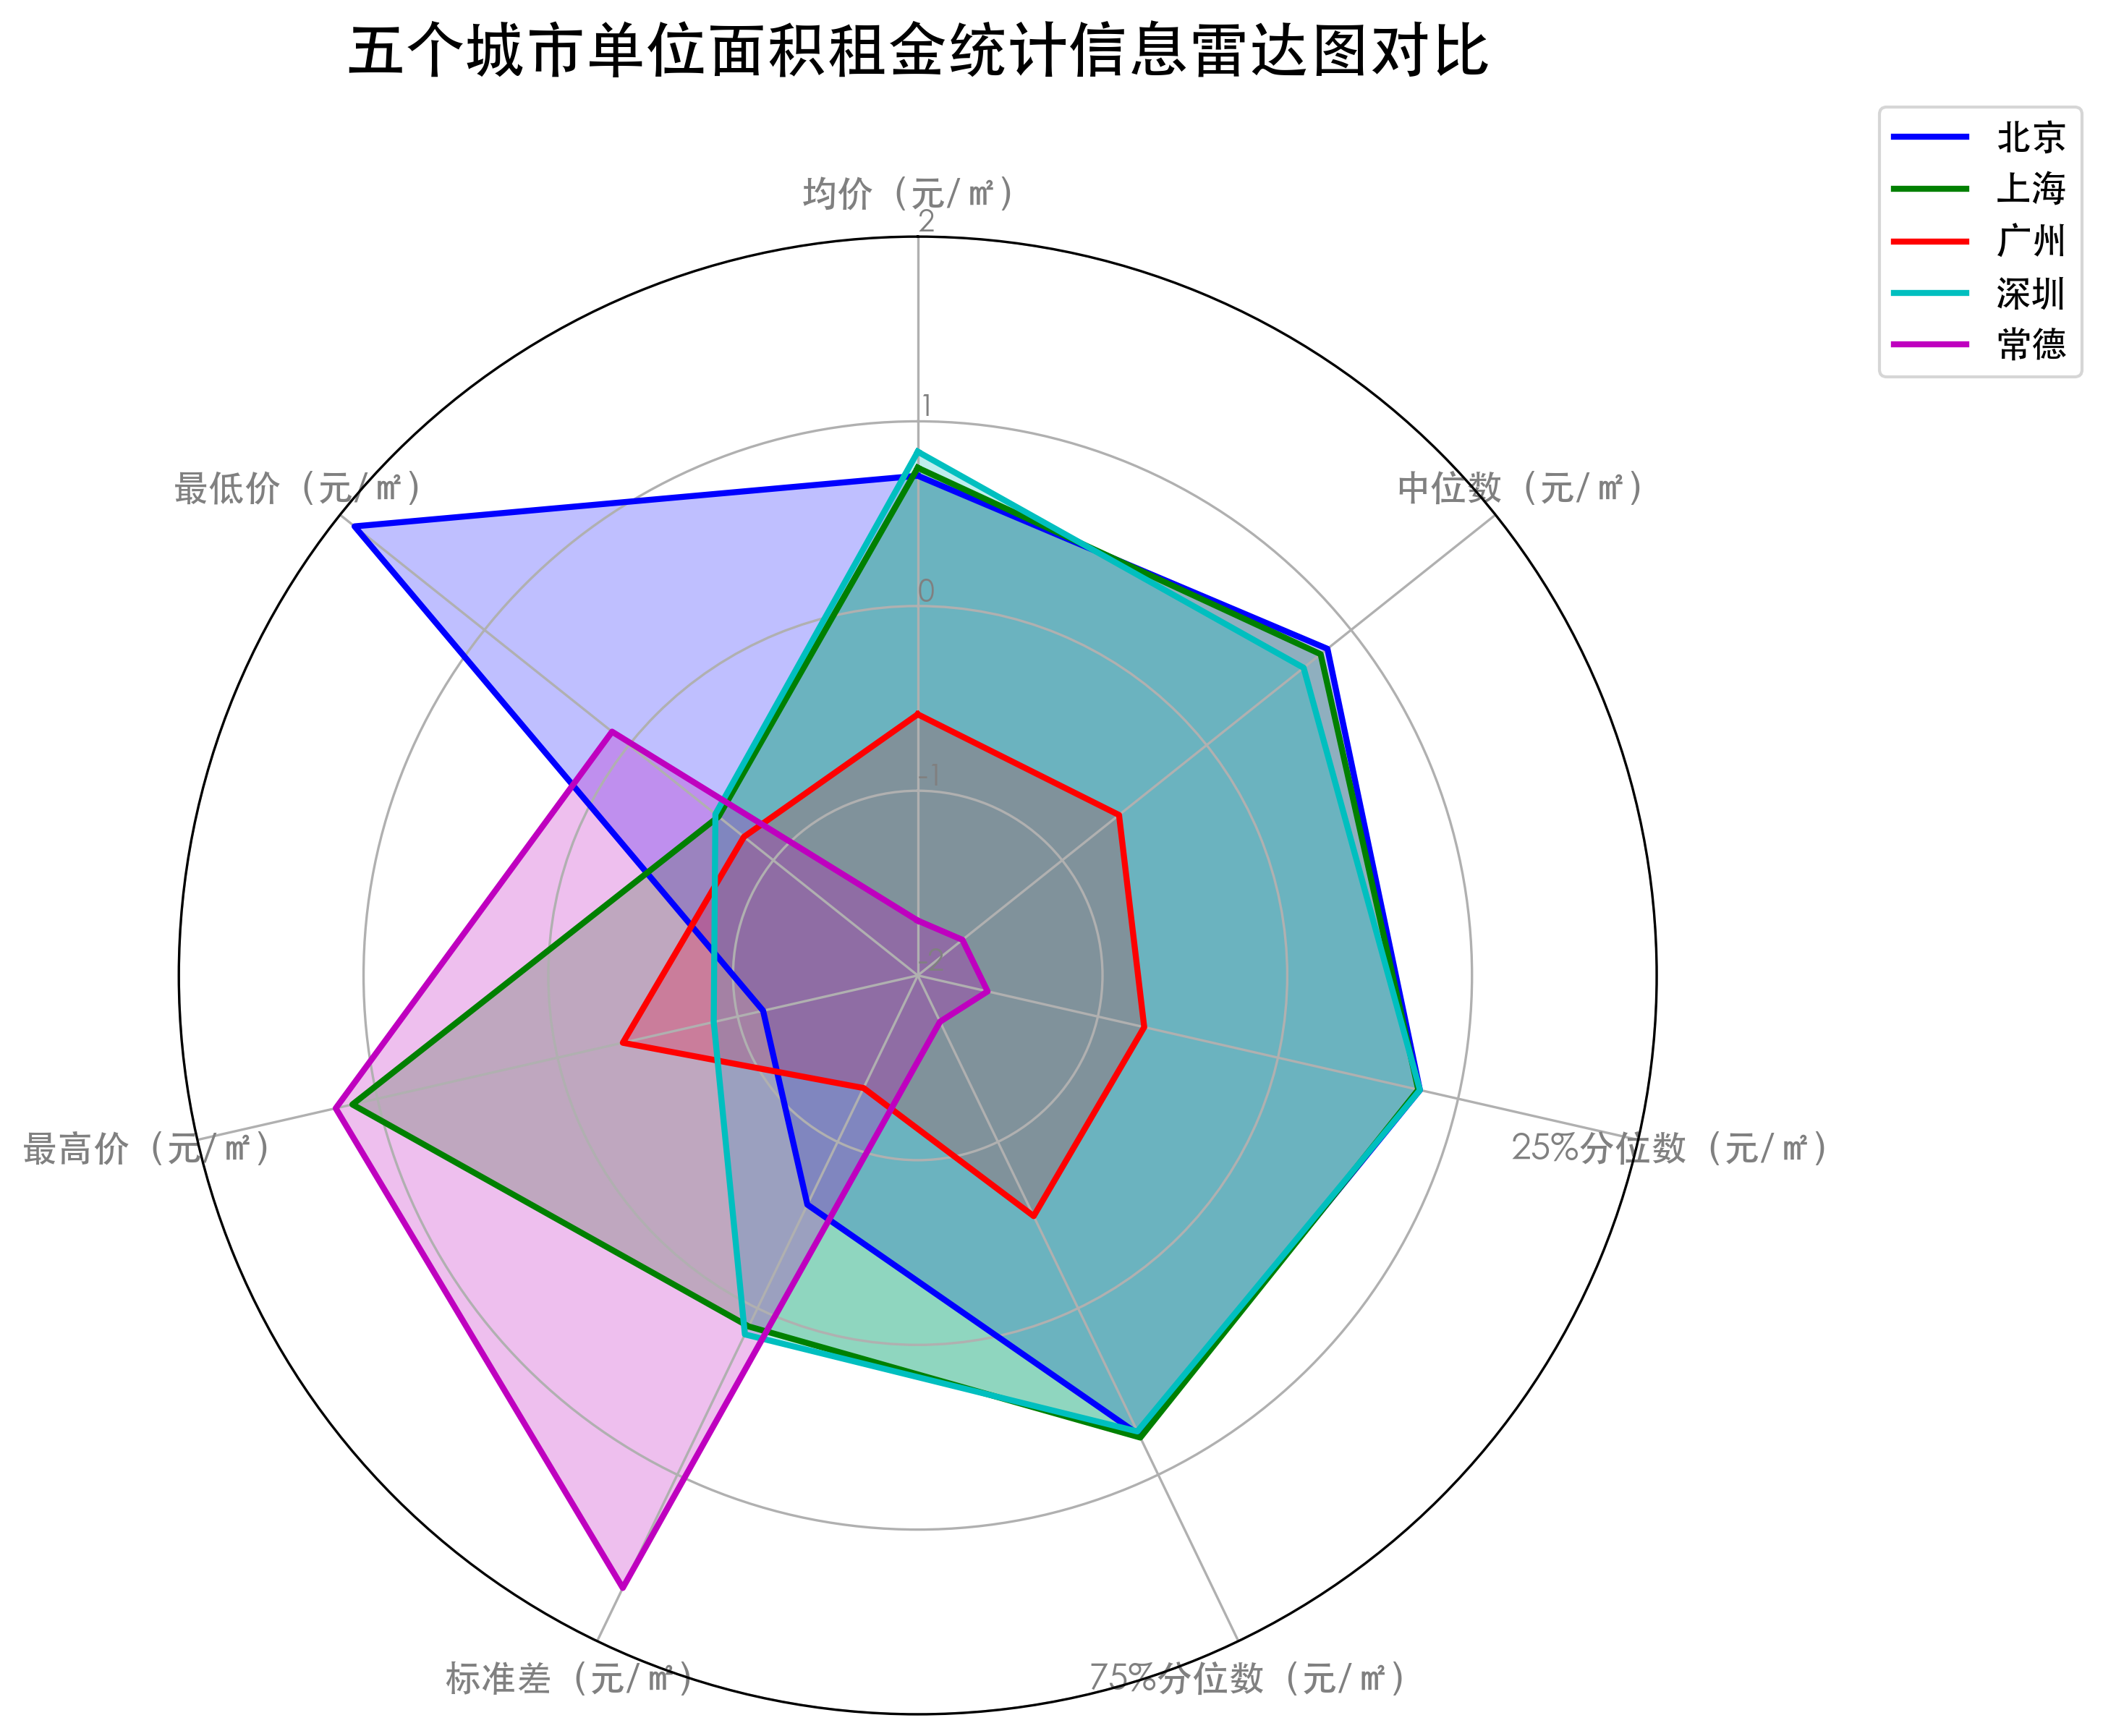
\includegraphics[width=0.7\linewidth]{../../figure/unit_price_radar_chart.png}
    \caption{五个城市单位面积租金统计信息雷达图对比}
    \label{fig:unit_price_radar_chart}
\end{figure}

\subsection{居室分析}
首先通过直方图展示不同城市的一居、二居、三居租金信息,进行城市间的比较。如图~\ref{fig:room_1_price_bar_chart}、图~\ref{fig:room_2_price_bar_chart}、图~\ref{fig:room_3_price_bar_chart}。
\begin{figure}[htbp]
    \centering
    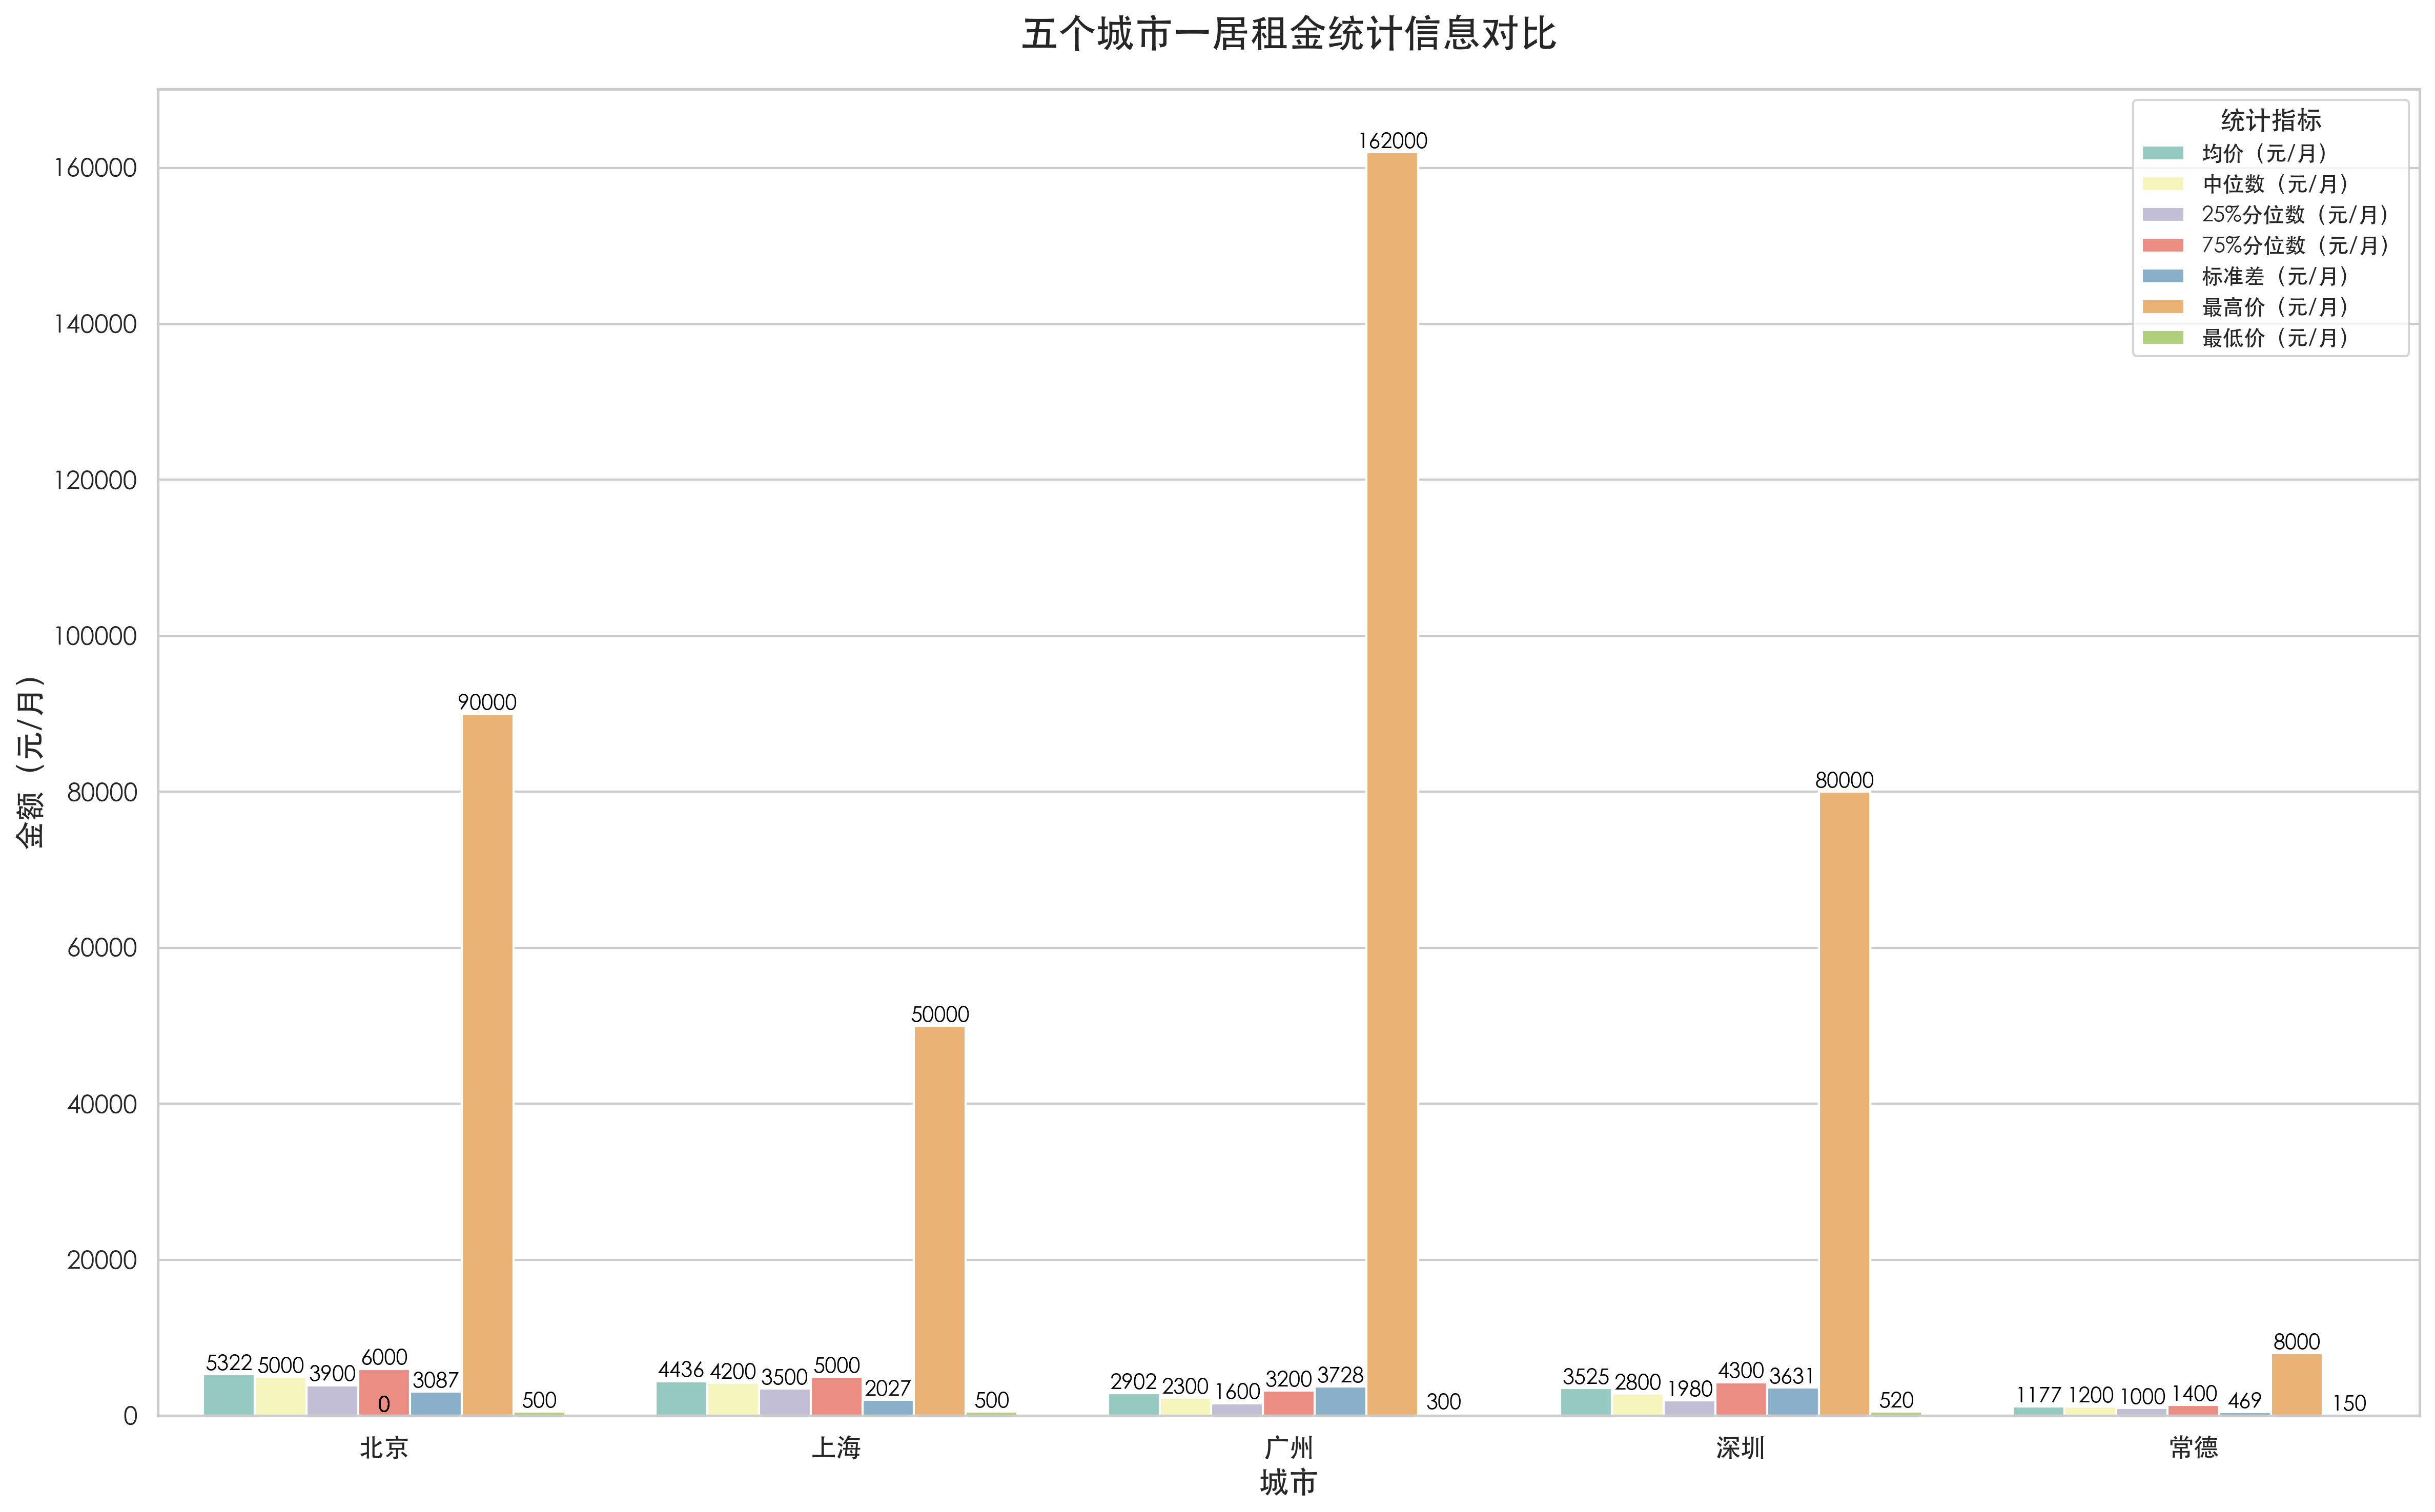
\includegraphics[width=0.7\linewidth]{../../figure/room_1_price_bar_chart.png}
    \caption{五个城市一居租金统计信息对比}
    \label{fig:room_1_price_bar_chart}
\end{figure}
\begin{figure}[htbp]
    \centering
    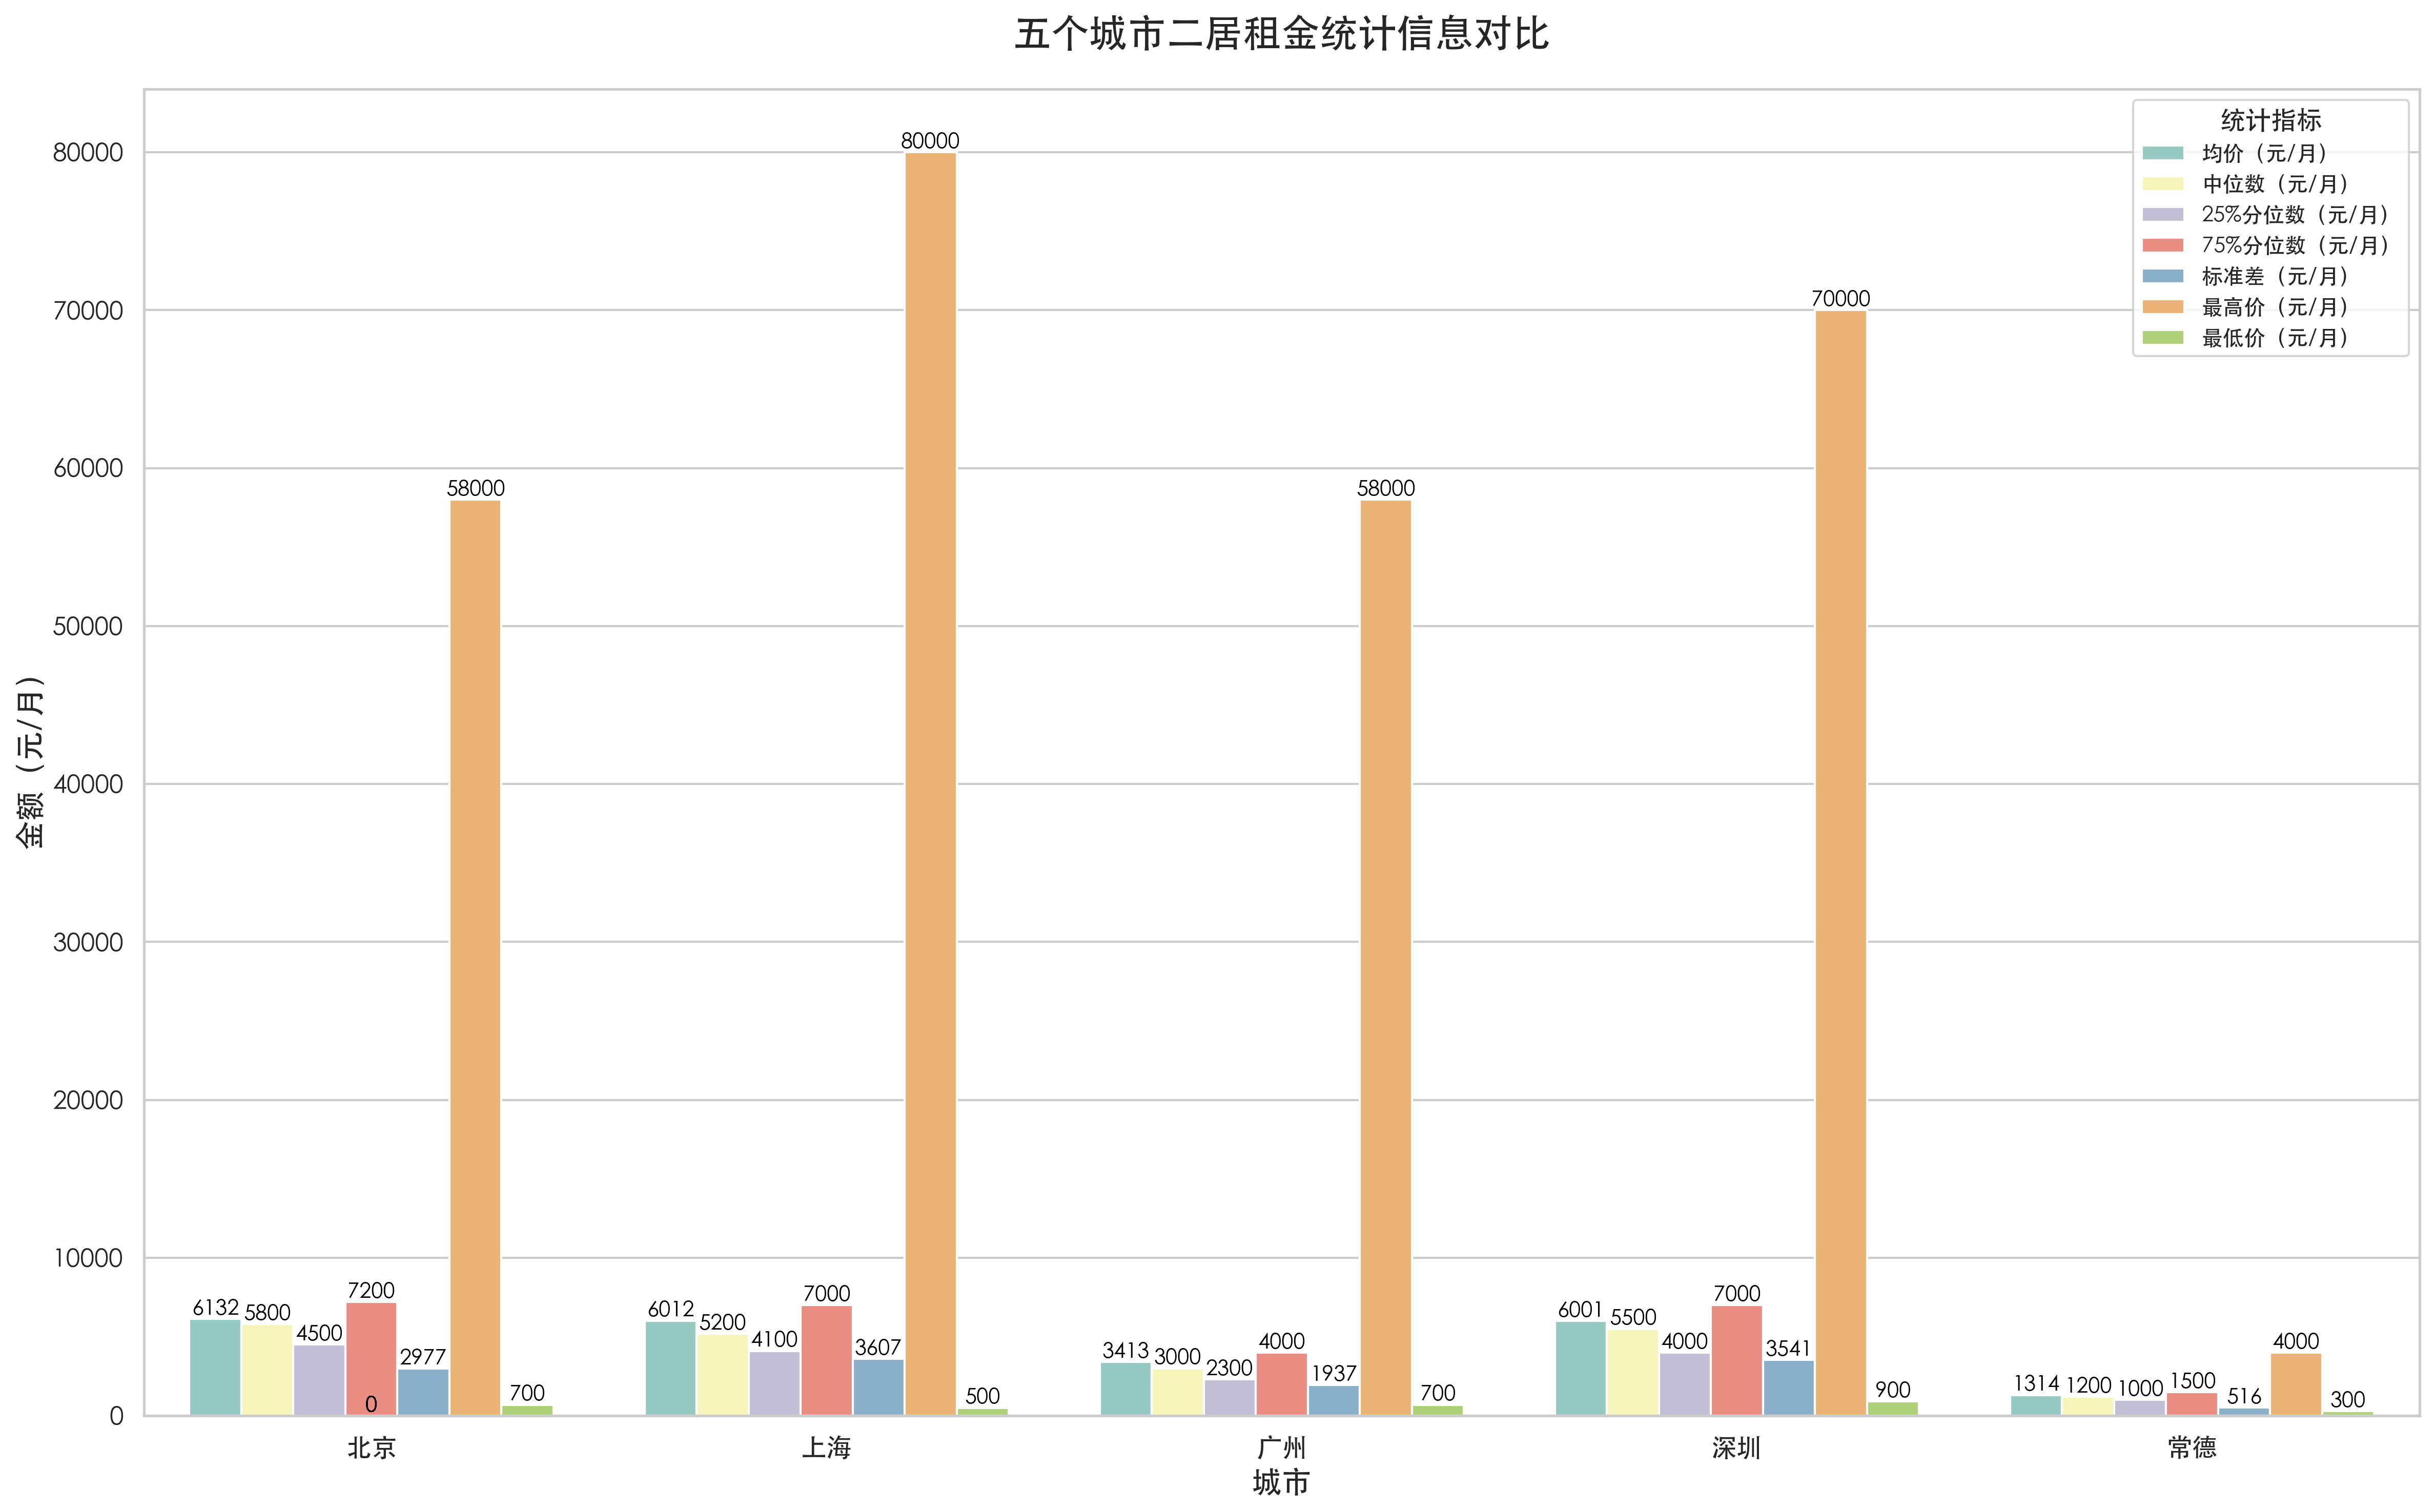
\includegraphics[width=0.7\linewidth]{../../figure/room_2_price_bar_chart.png}
    \caption{五个城市二居租金统计信息对比}
    \label{fig:room_2_price_bar_chart}
\end{figure}
\begin{figure}[htbp]
    \centering
    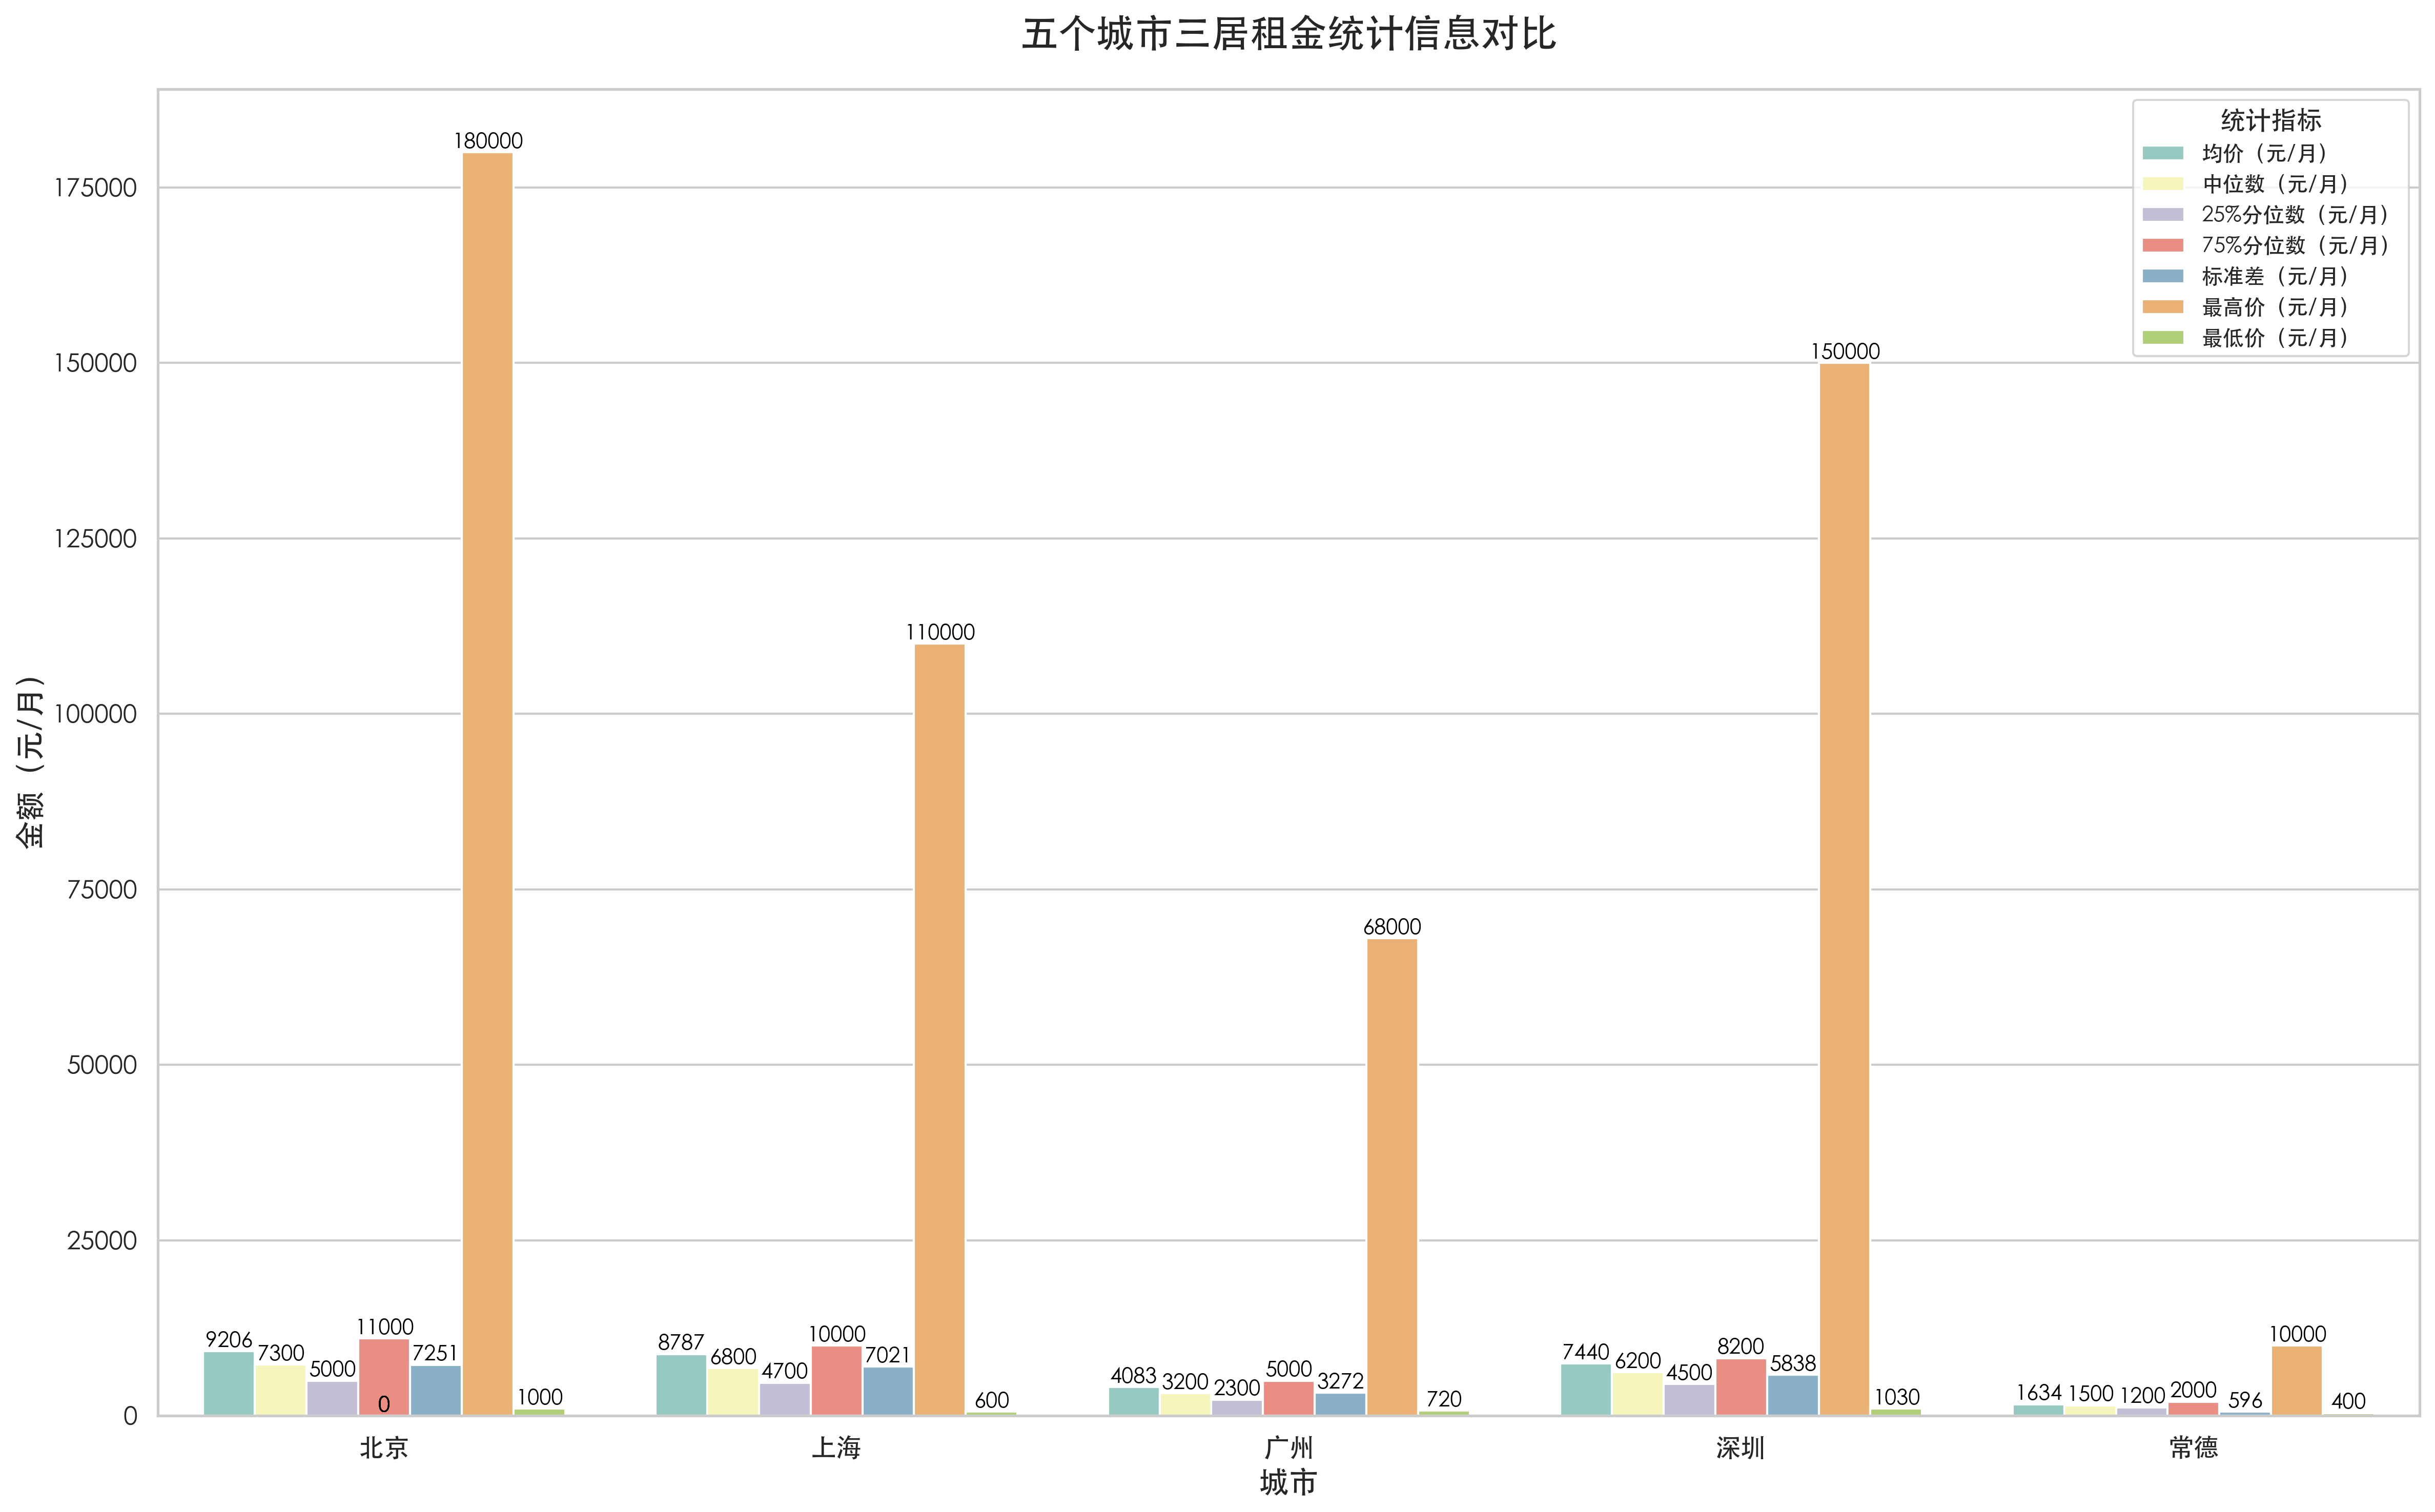
\includegraphics[width=0.7\linewidth]{../../figure/room_3_price_bar_chart.png}
    \caption{五个城市三居租金统计信息对比}
    \label{fig:room_3_price_bar_chart}
\end{figure}

然后通过折线图进行城市内的比较,观察随着房室增加的变化情况。如图~\ref{fig:bj_room_price_line_chart}、图~\ref{fig:sh_room_price_line_chart}、图~\ref{fig:gz_room_price_line_chart}、图~\ref{fig:sz_room_price_line_chart}、图~\ref{fig:changde_room_price_line_chart}。
\begin{figure}[htbp]
    \centering
    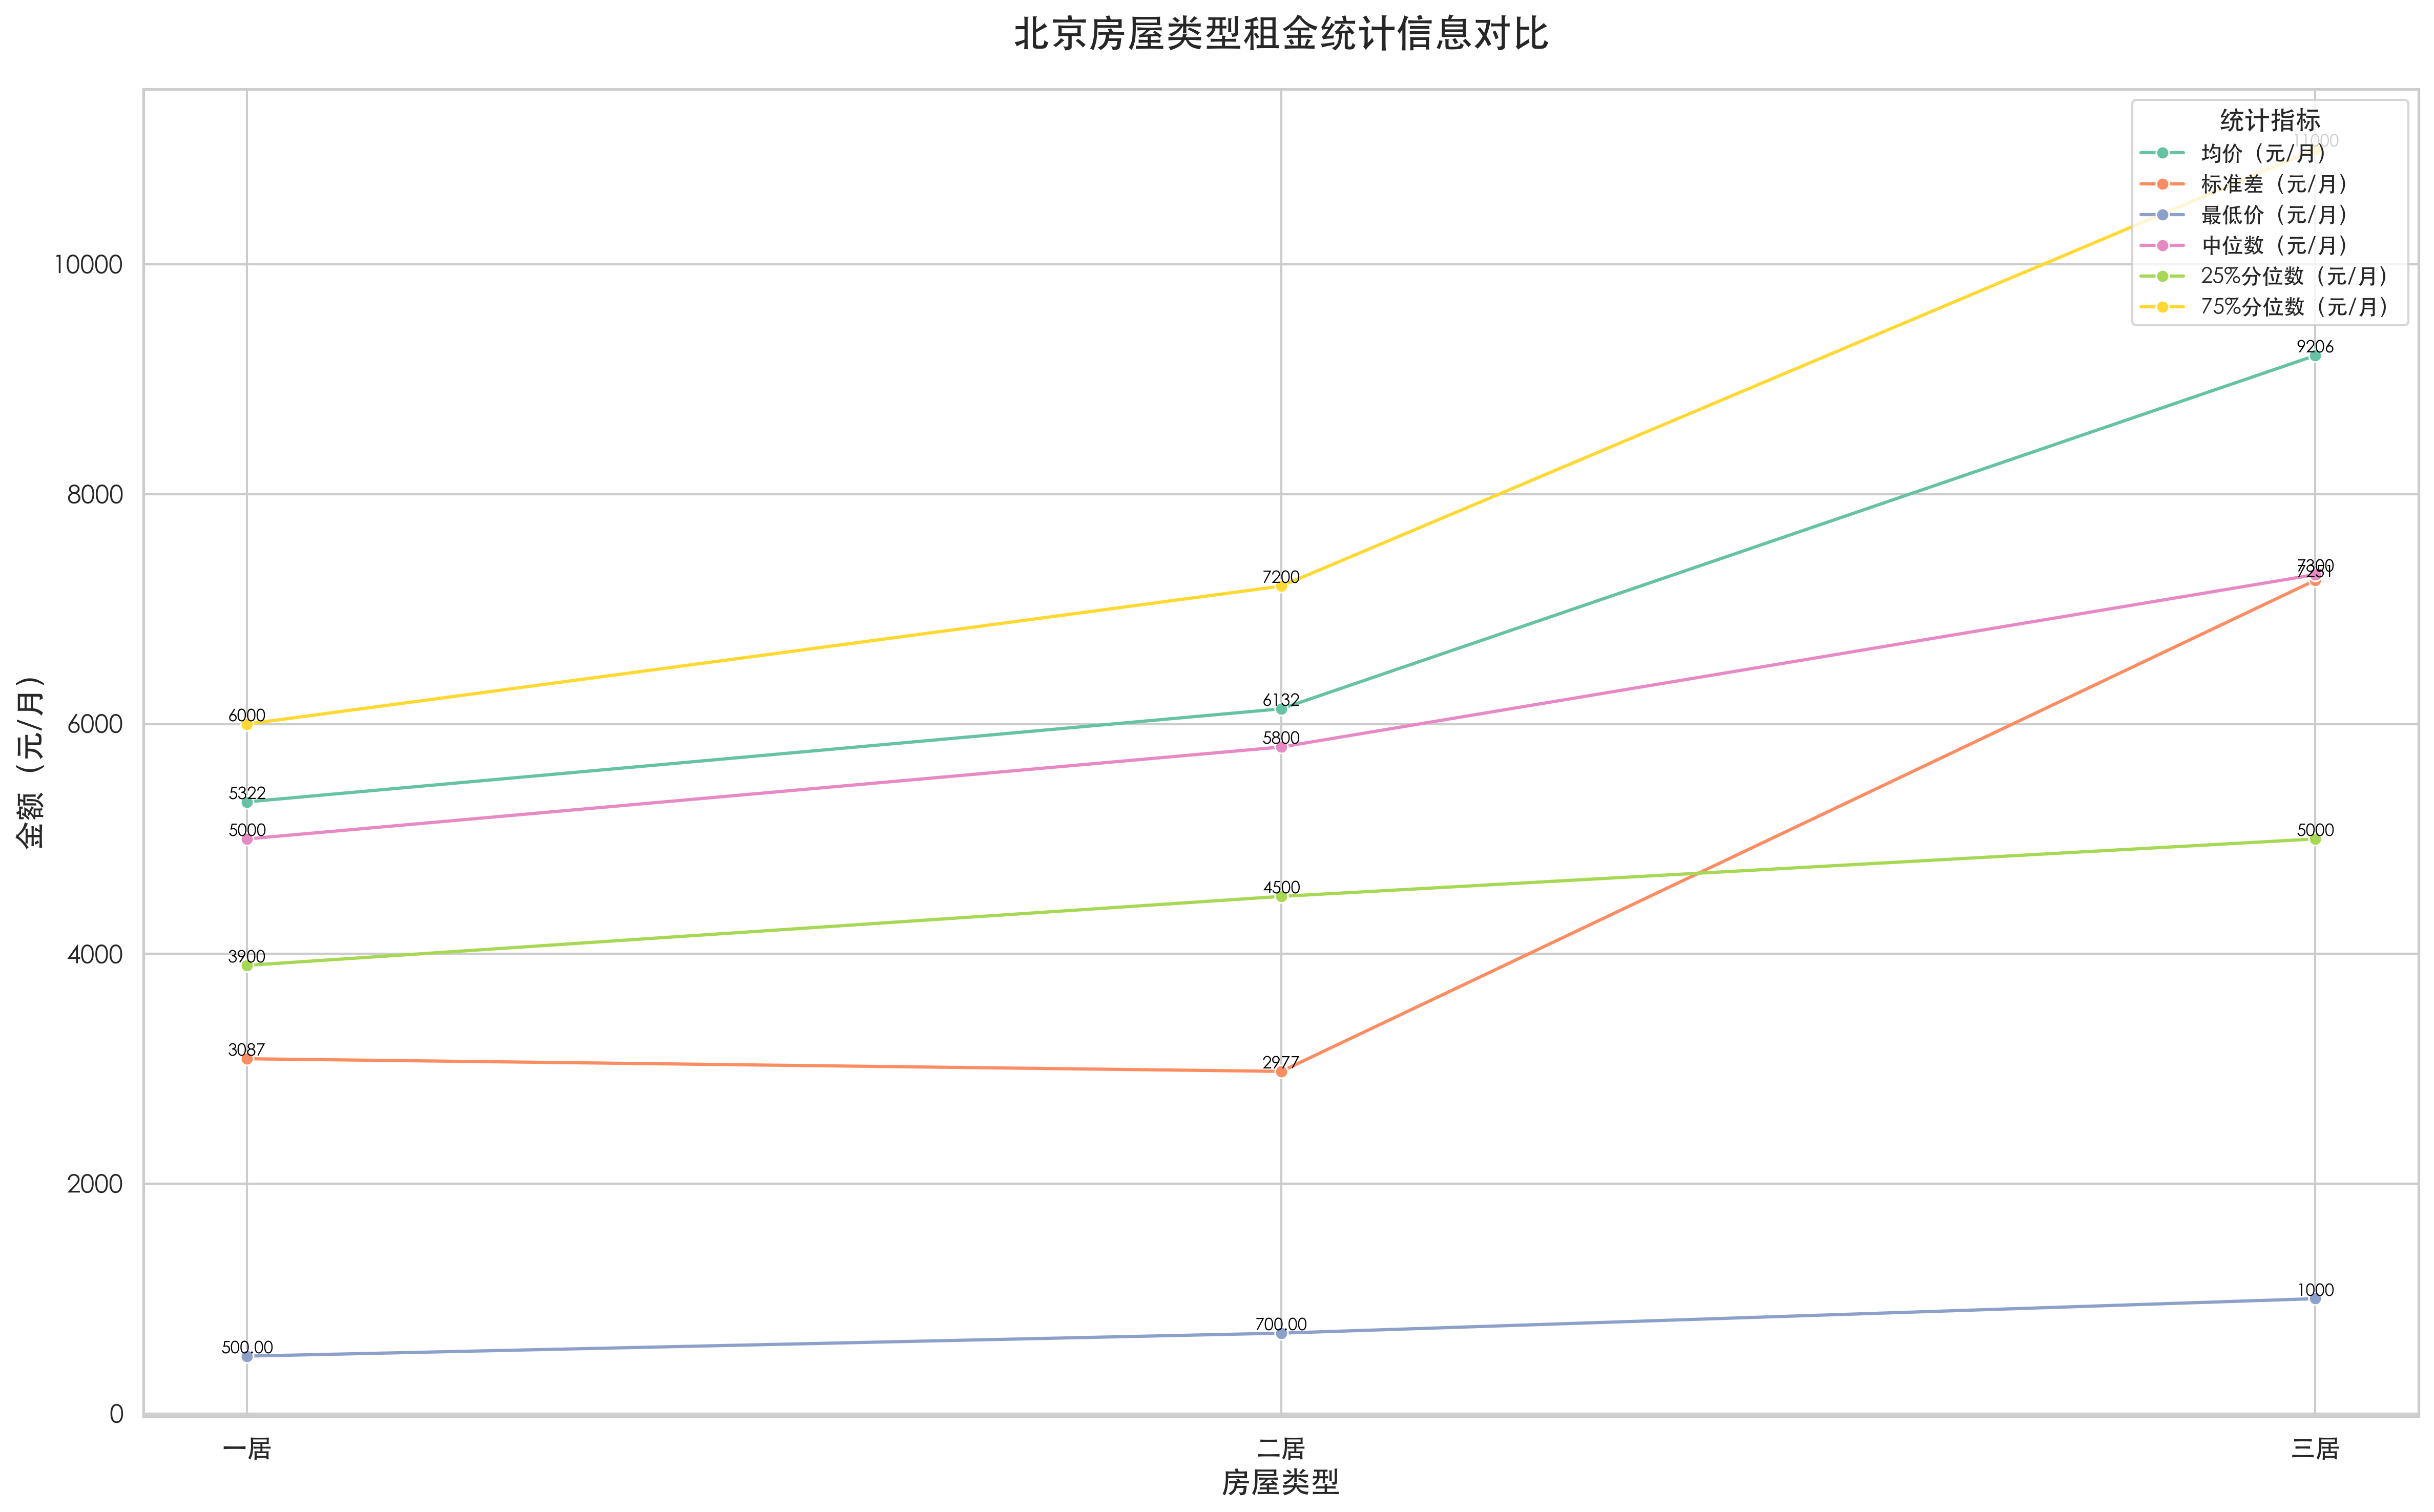
\includegraphics[width=0.7\linewidth]{../../figure/bj_room_price_line_chart.png}
    \caption{北京房屋类型租金信息对比}
    \label{fig:bj_room_price_line_chart}
\end{figure}
\begin{figure}[htbp]
    \centering
    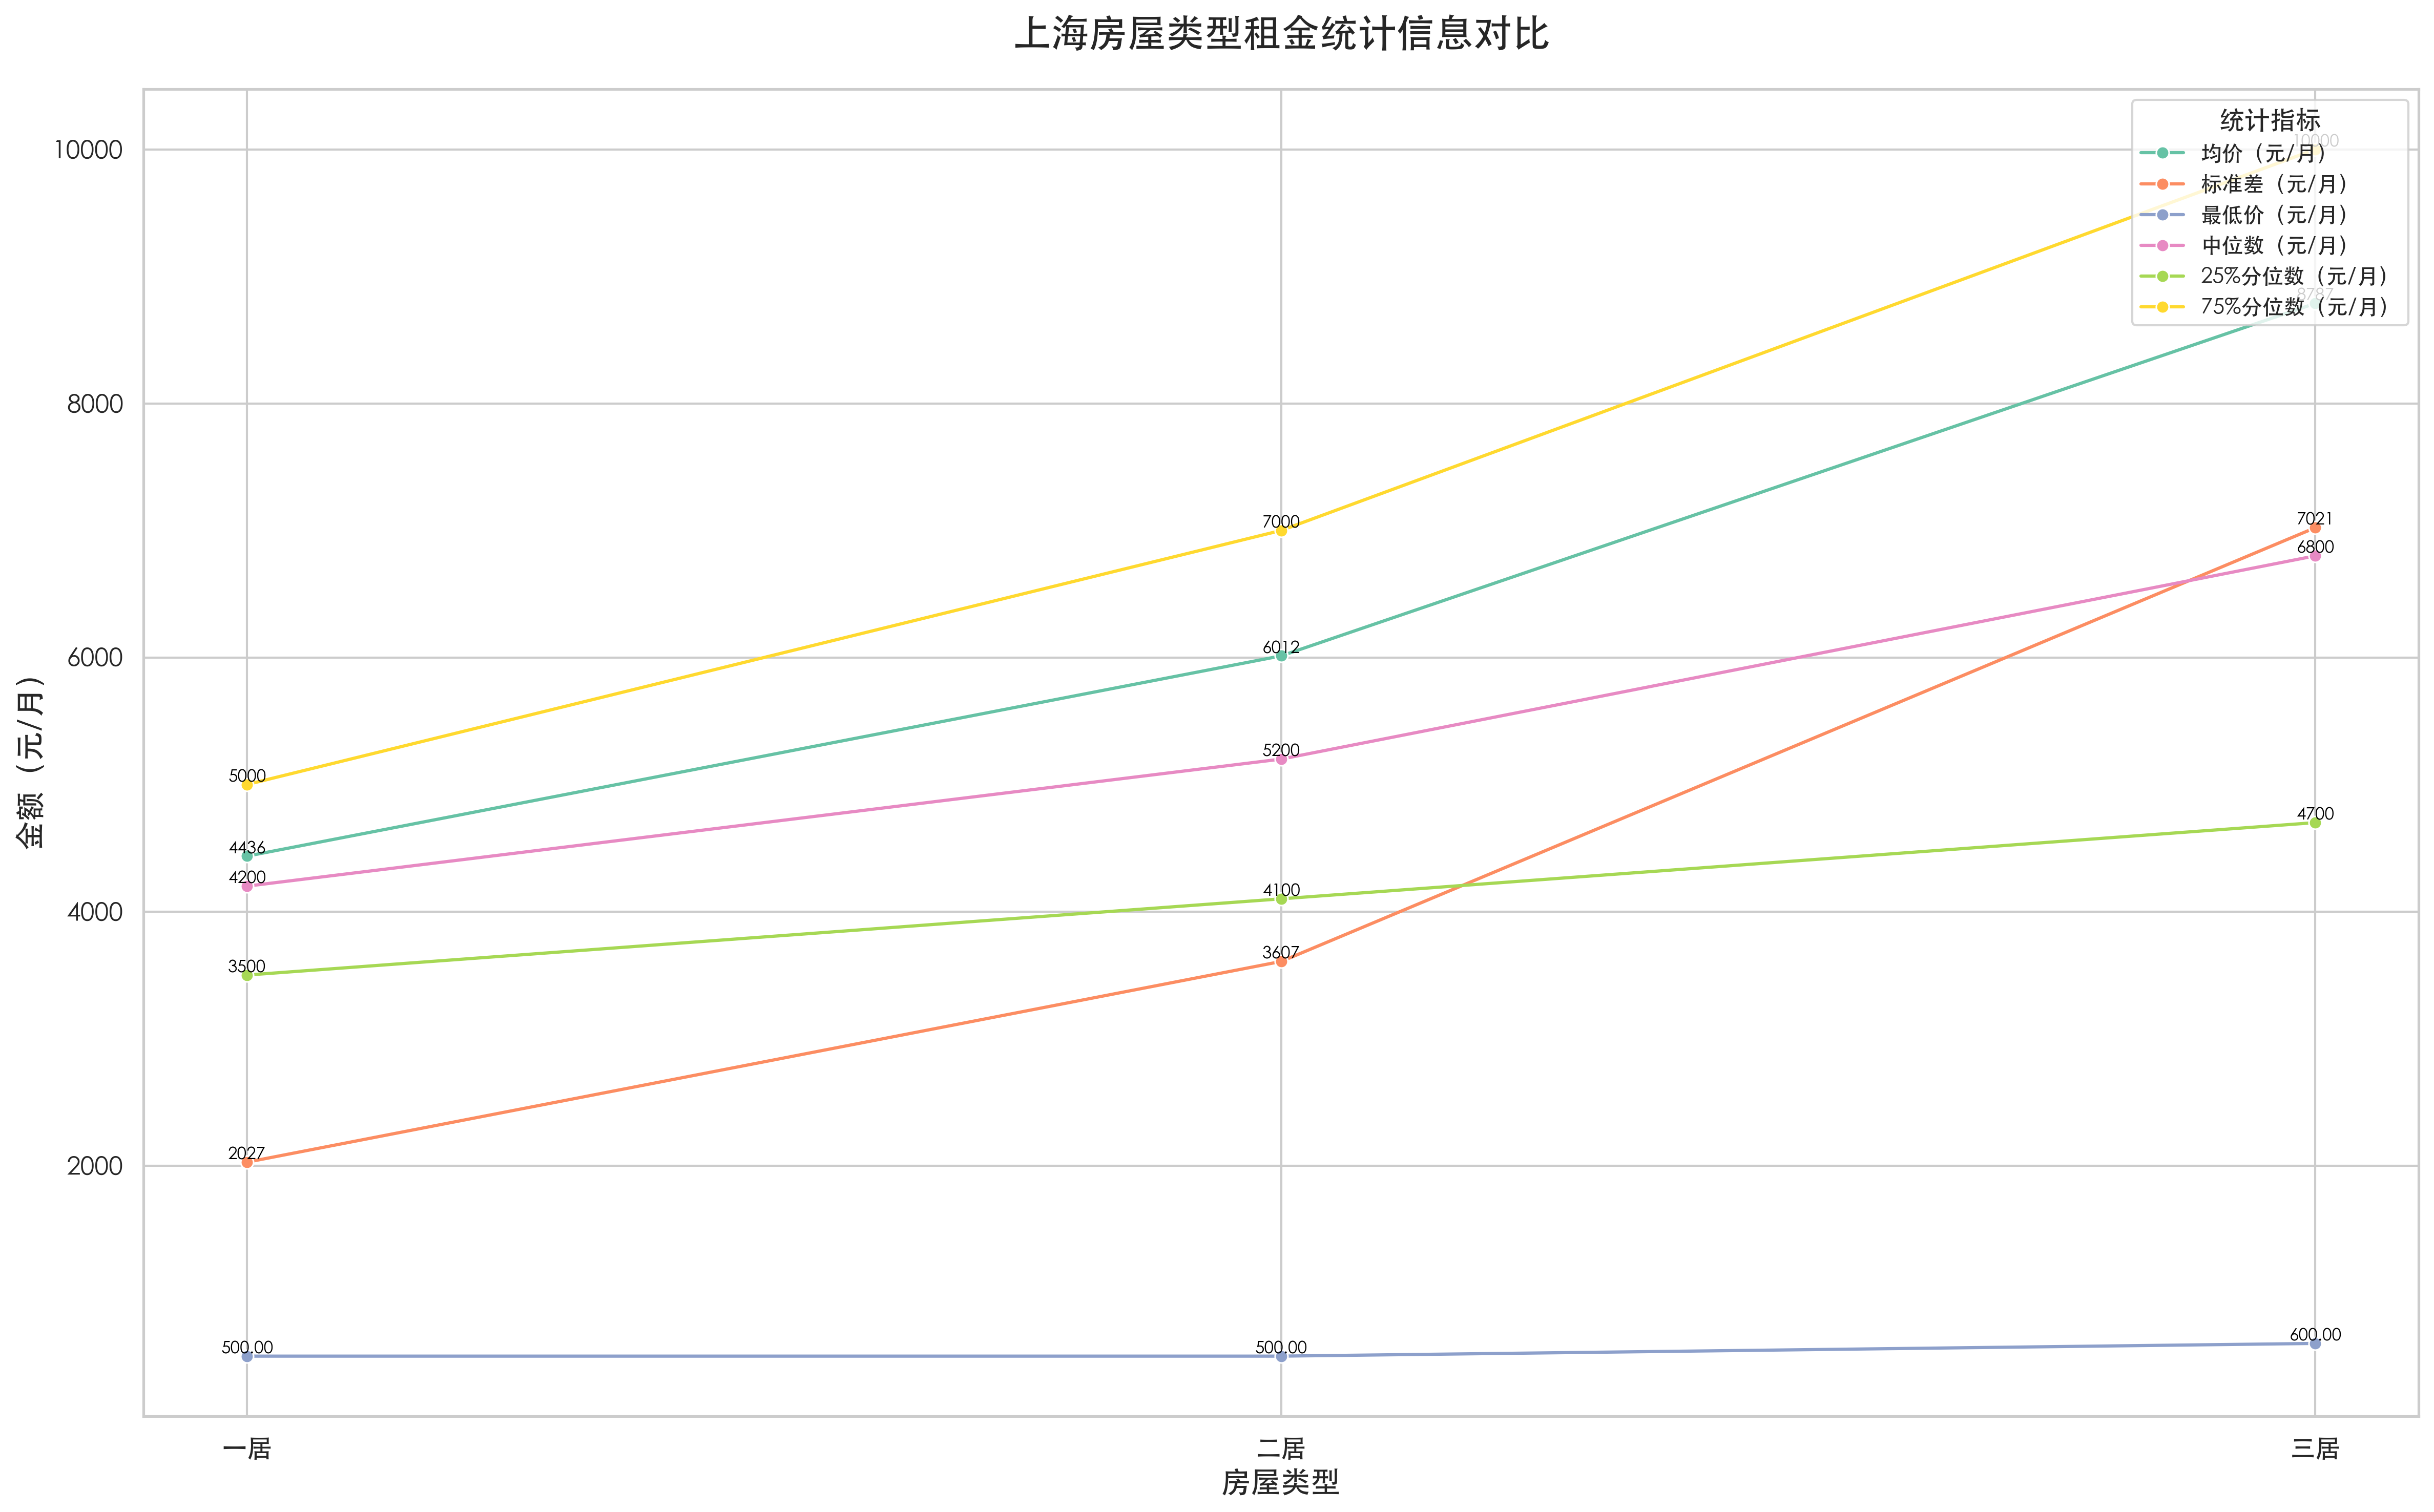
\includegraphics[width=0.7\linewidth]{../../figure/sh_room_price_line_chart.png}
    \caption{上海房屋类型租金信息对比}
    \label{fig:sh_room_price_line_chart}
\end{figure}
\begin{figure}[htbp]
    \centering
    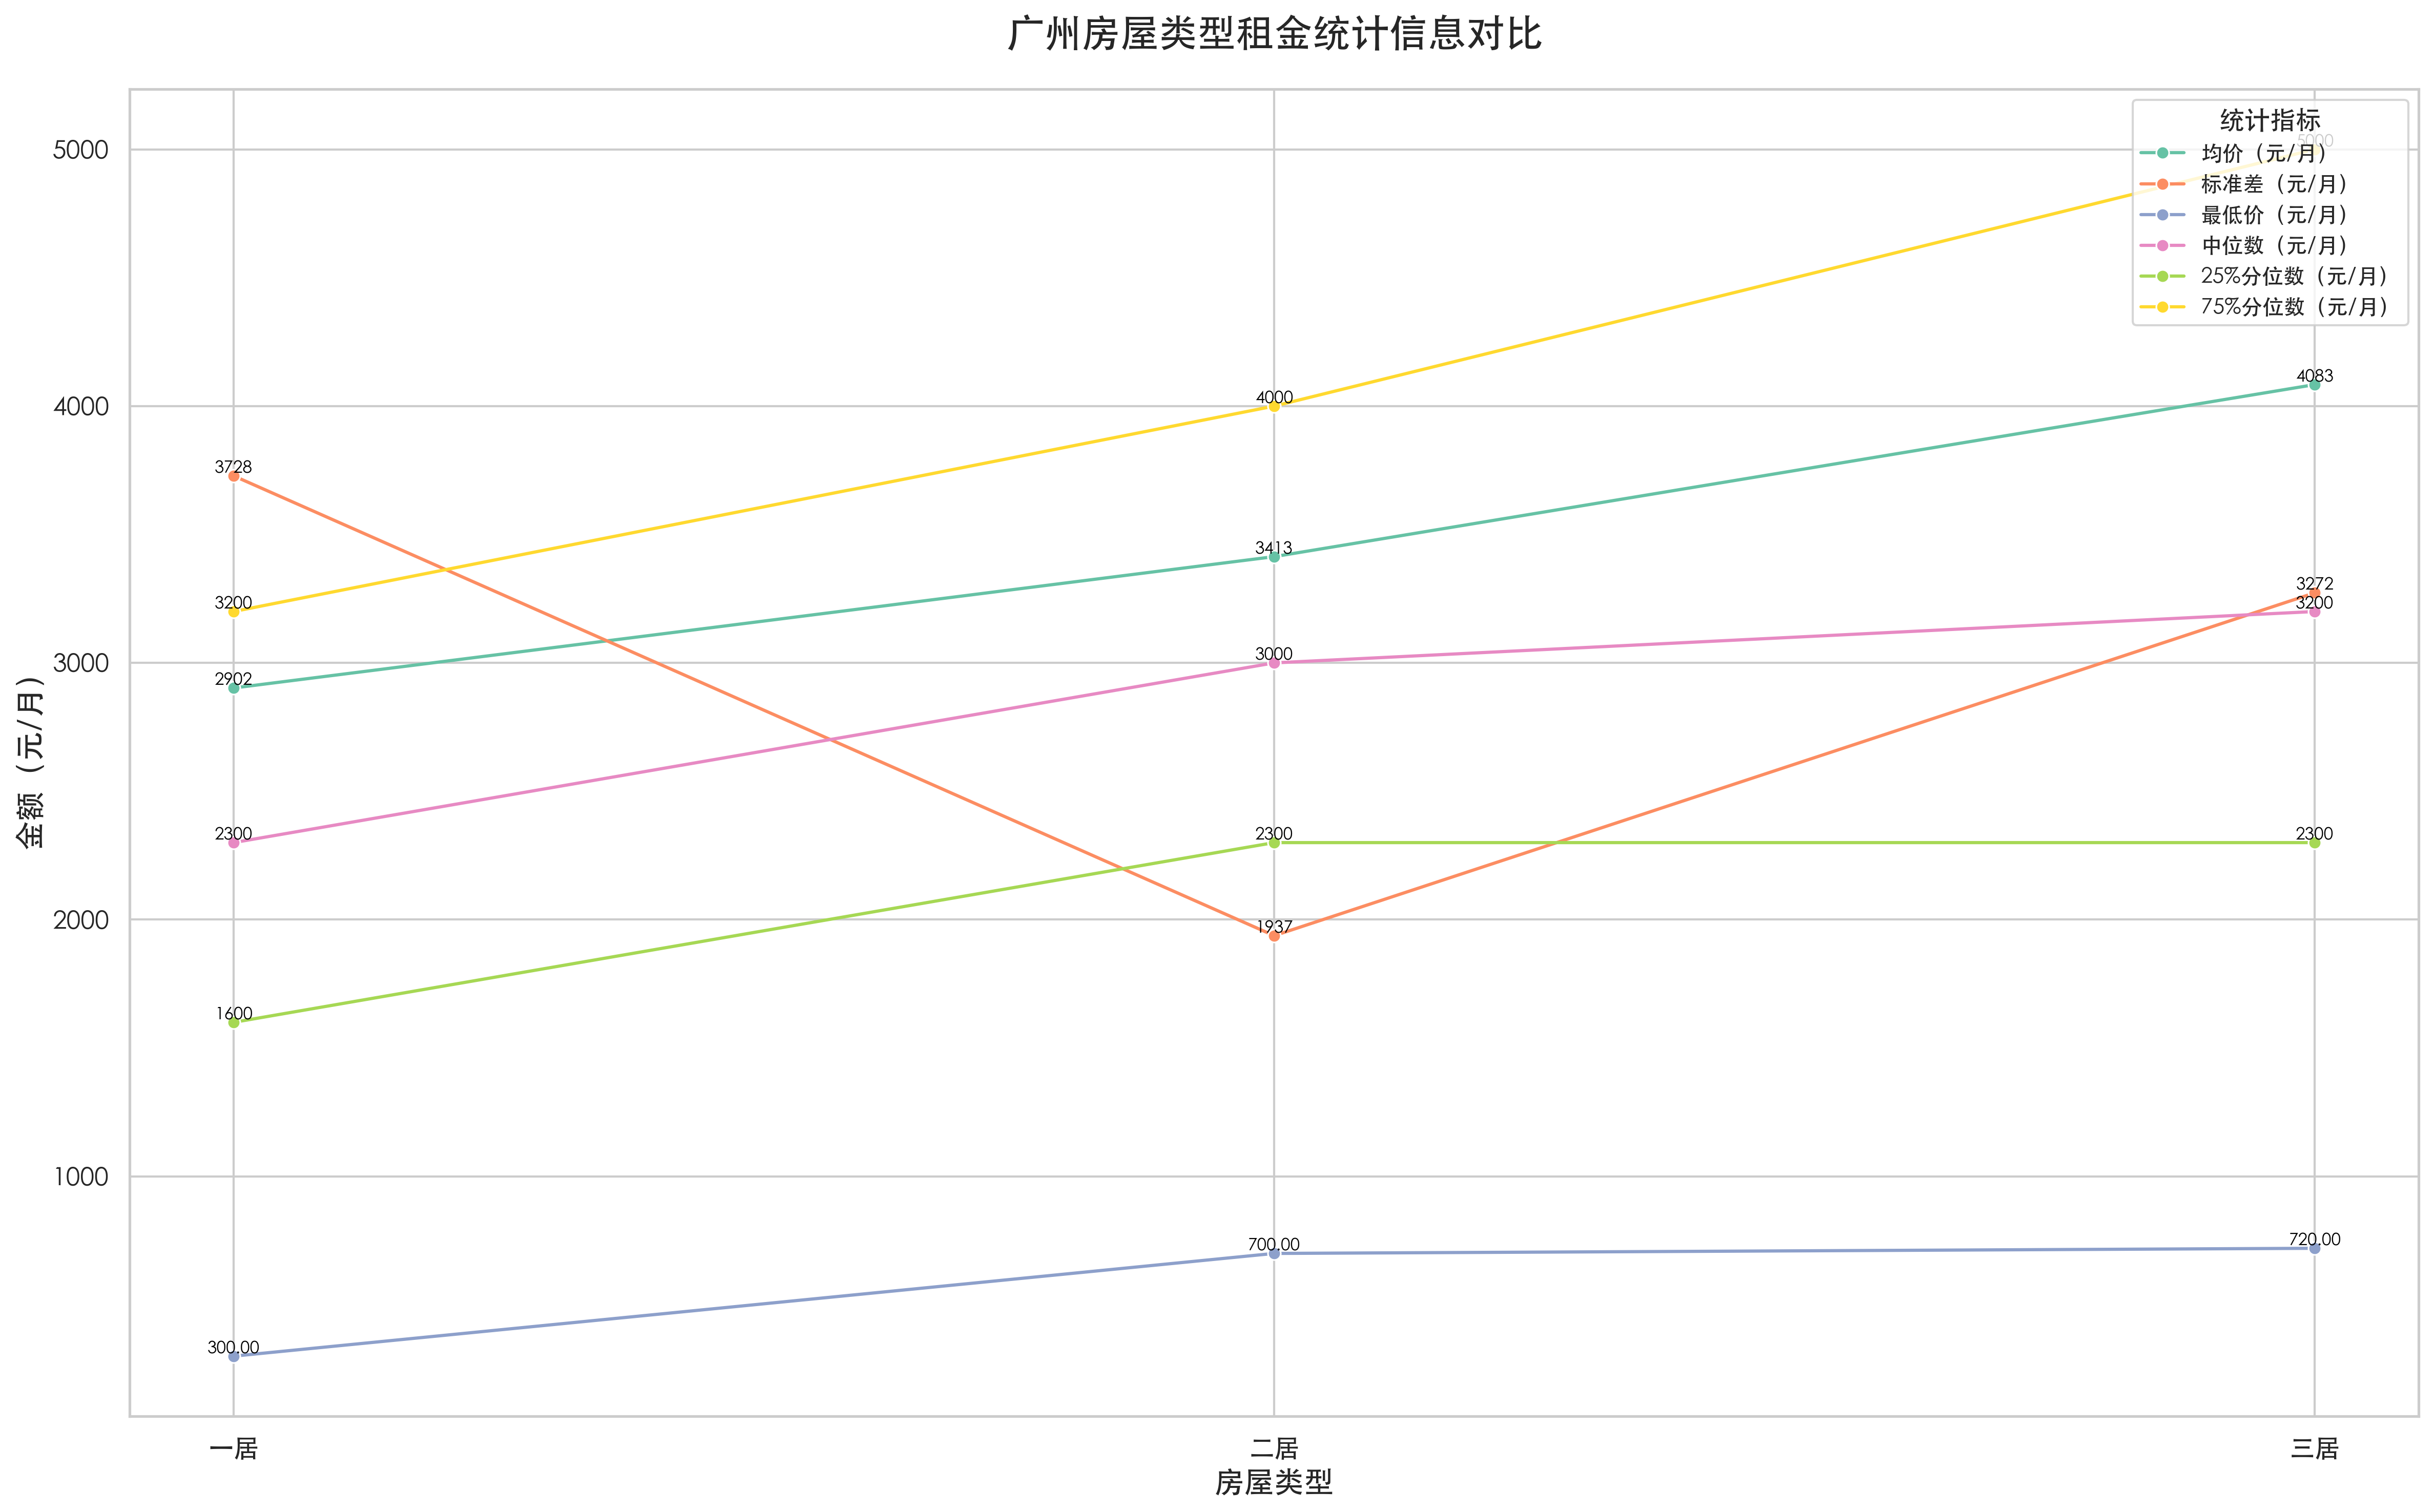
\includegraphics[width=0.7\linewidth]{../../figure/gz_room_price_line_chart.png}
    \caption{广州房屋类型租金信息对比}
    \label{fig:gz_room_price_line_chart}
\end{figure}
\begin{figure}[htbp]
    \centering
    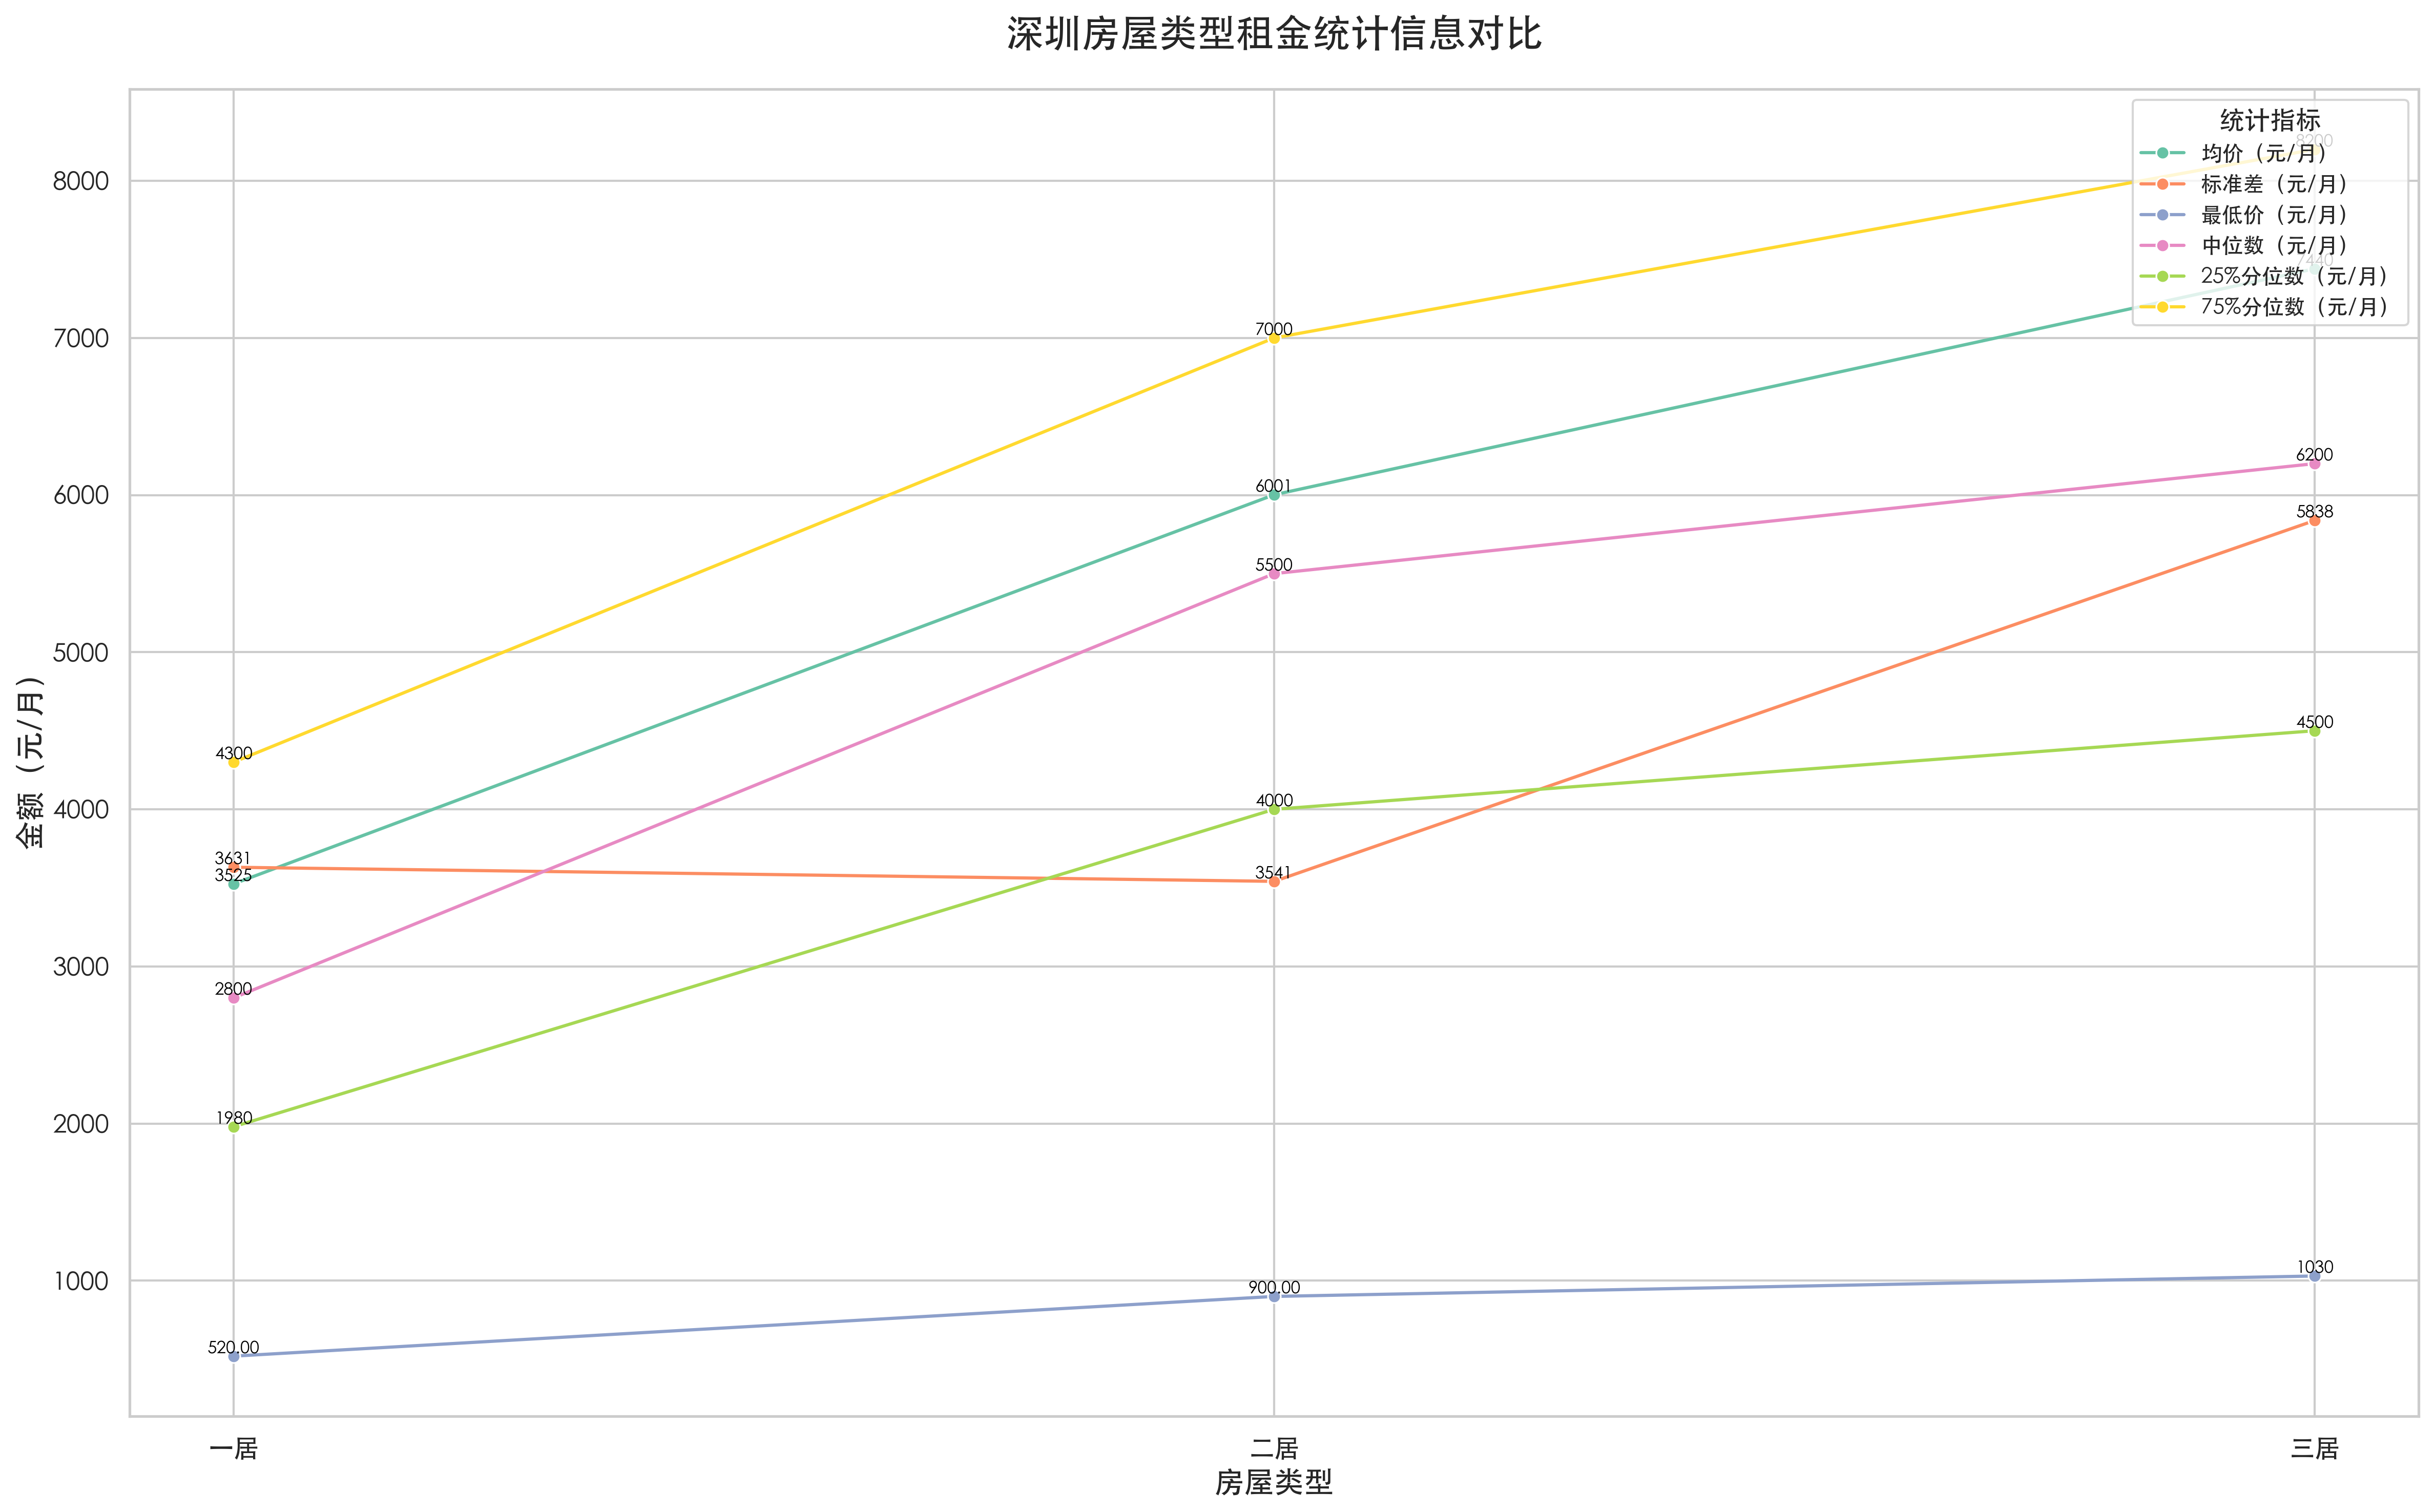
\includegraphics[width=0.7\linewidth]{../../figure/sz_room_price_line_chart.png}
    \caption{深圳房屋类型租金信息对比}
    \label{fig:sz_room_price_line_chart}
\end{figure}
\begin{figure}[htbp]
    \centering
    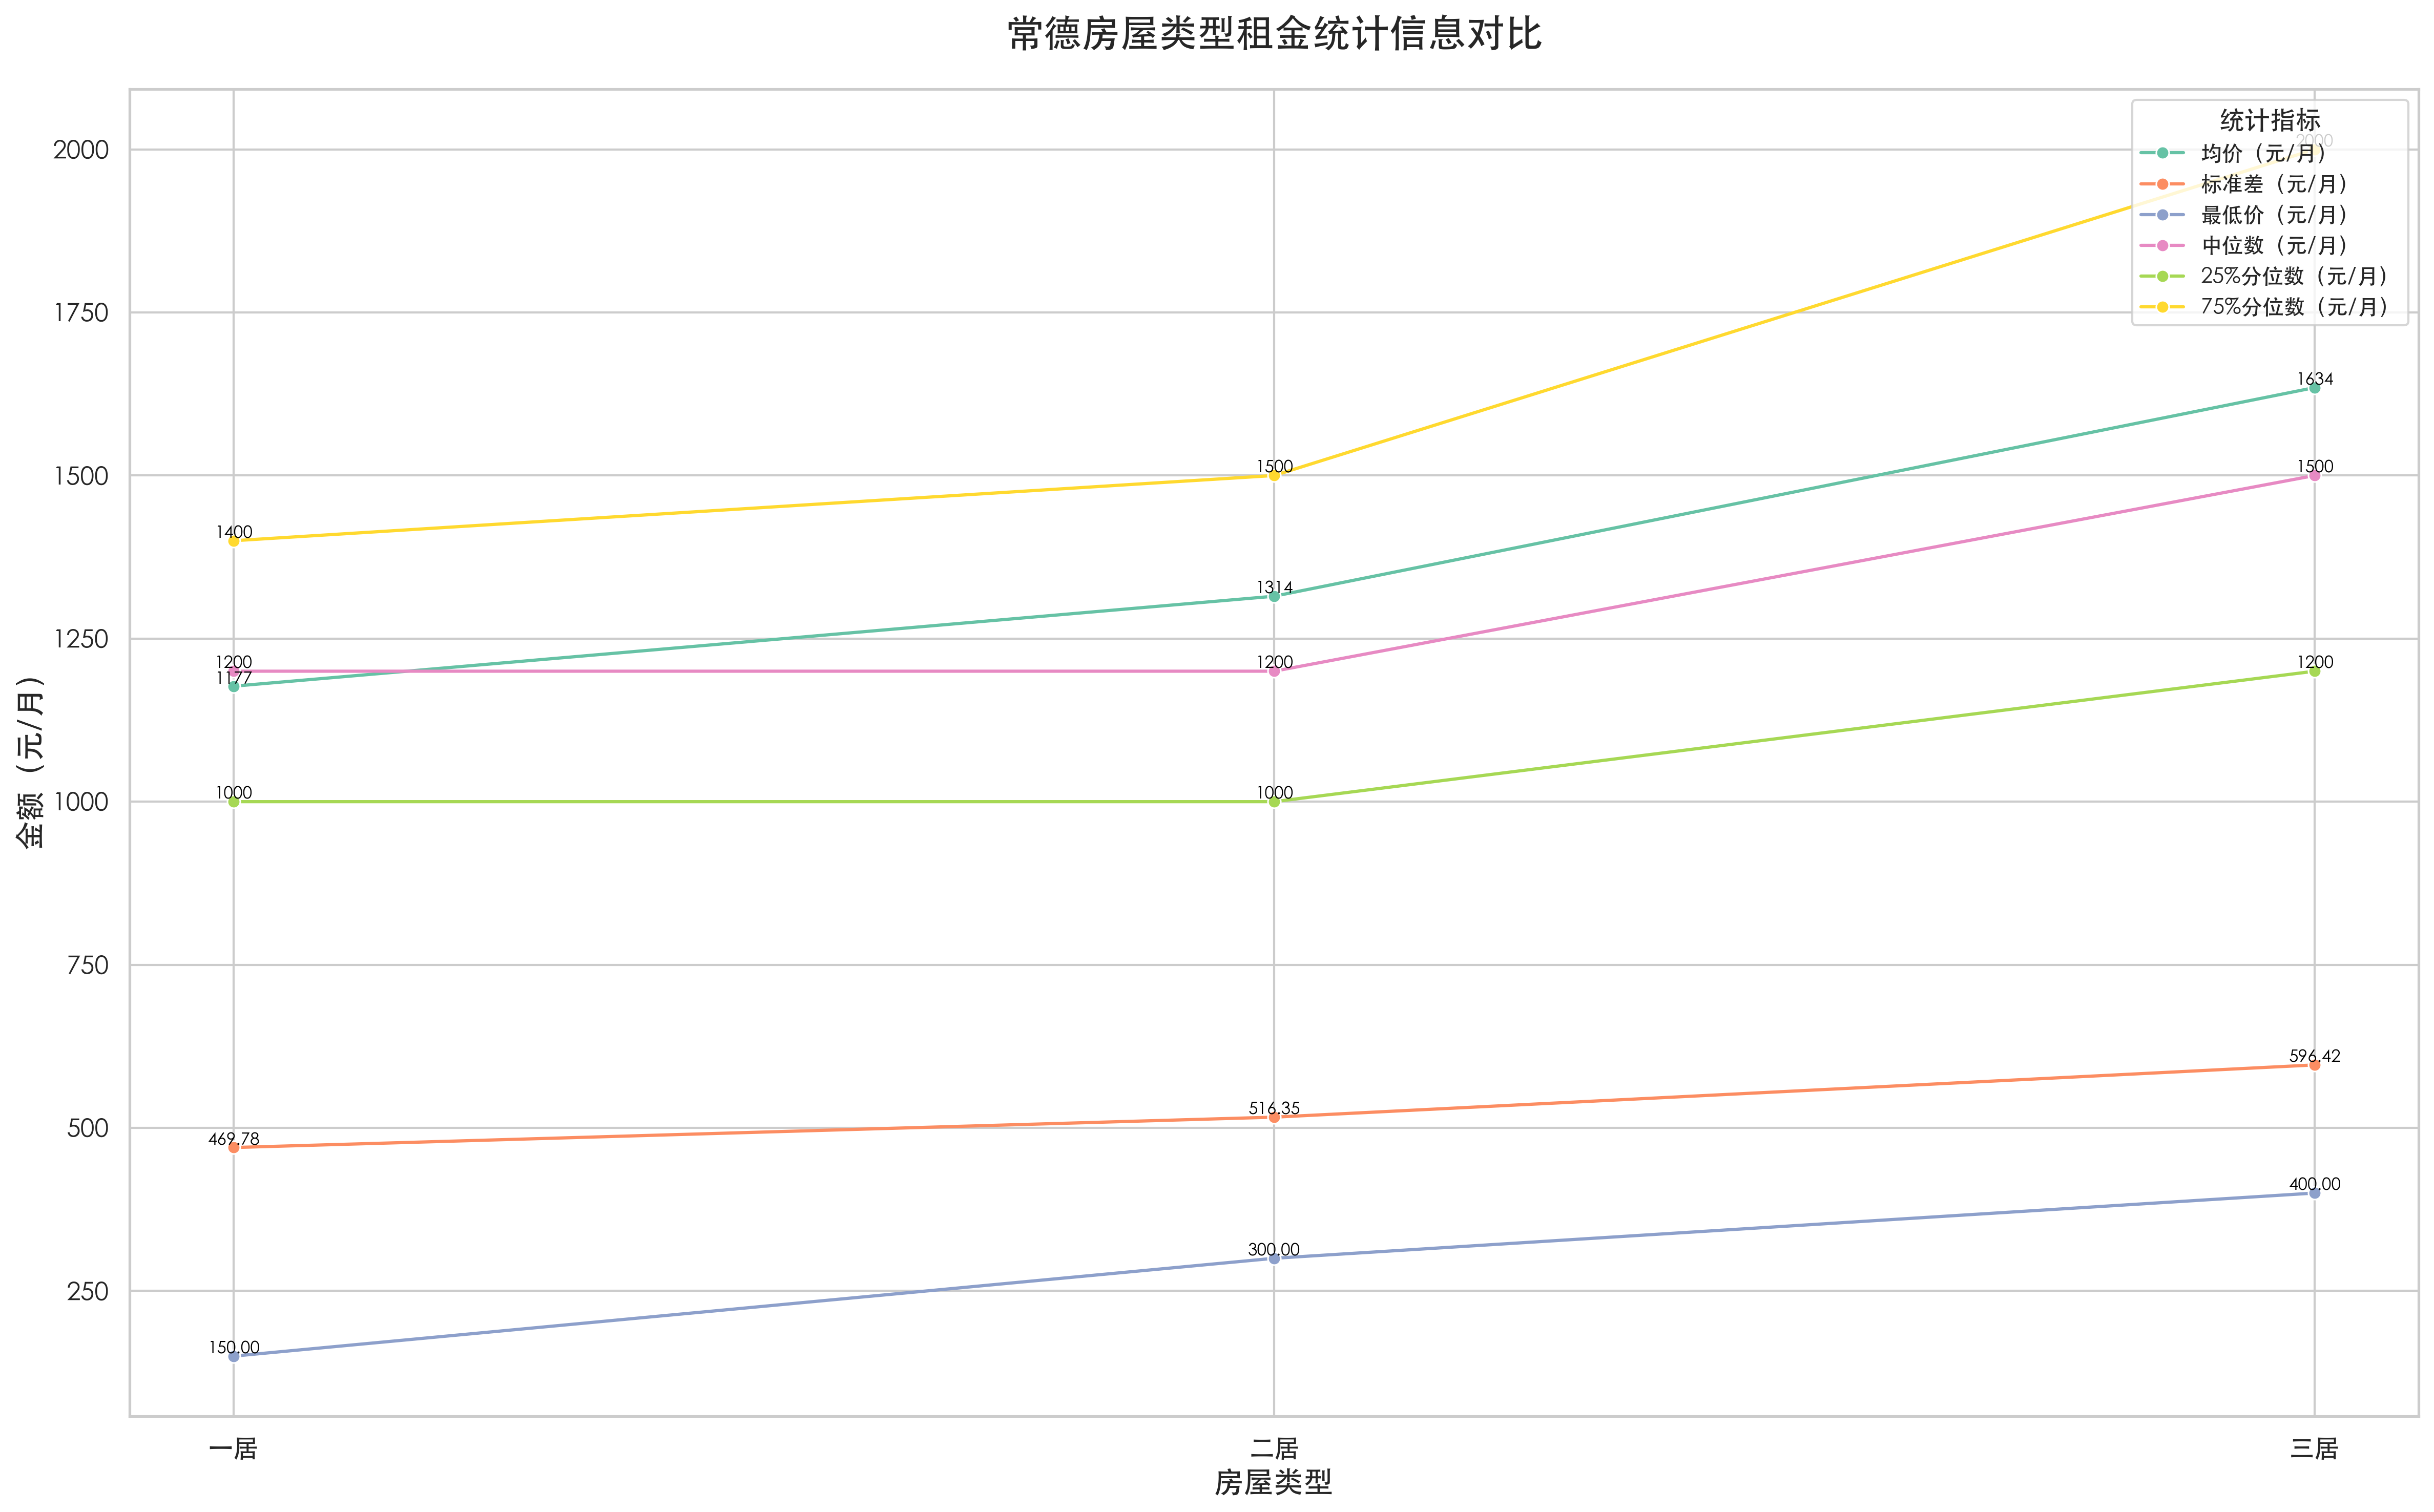
\includegraphics[width=0.7\linewidth]{../../figure/changde_room_price_line_chart.png}
    \caption{常德房屋类型租金信息对比}
    \label{fig:changde_room_price_line_chart}
\end{figure}

\subsection{板块分析}
通过直方图之间展示板块租金信息,画图前对板块的租金进行排序,便于比较。如图~\ref{fig:bj_area_price_bar_chart}、图~\ref{fig:sh_area_price_bar_chart}、图~\ref{fig:gz_area_price_bar_chart}、图~\ref{fig:sz_area_price_bar_chart}、图~\ref{fig:changde_area_price_bar_chart}。
\begin{figure}[htbp]
    \centering
    \includegraphics[width=0.7\linewidth]{../../figure/bj_area_price_bar_chart.png}
    \caption{北京各板块平均租金对比}
    \label{fig:bj_area_price_bar_chart}
\end{figure}
\begin{figure}[htbp]
    \centering
    \includegraphics[width=0.7\linewidth]{../../figure/sh_area_price_bar_chart.png}
    \caption{上海各板块平均租金对比}
    \label{fig:sh_area_price_bar_chart}
\end{figure}
\begin{figure}[htbp]
    \centering
    \includegraphics[width=0.7\linewidth]{../../figure/gz_area_price_bar_chart.png}
    \caption{广州各板块平均租金对比}
    \label{fig:gz_area_price_bar_chart}
\end{figure}
\begin{figure}[htbp]
    \centering
    \includegraphics[width=0.7\linewidth]{../../figure/sz_area_price_bar_chart.png}
    \caption{深圳各板块平均租金对比}
    \label{fig:sz_area_price_bar_chart}
\end{figure}
\begin{figure}
    \centering
    \includegraphics[width=0.7\linewidth]{../../figure/changde_area_price_bar_chart.png}
    \caption{常德各板块平均租金对比}
    \label{fig:changde_area_price_bar_chart}
\end{figure}

\subsubsection{区域分析}
由于板块数量众多,且直方图不够直观,采用在地图上的区域租金热力图展示,更直观地展示租金信息,并能结合地理位置进行分析。如图~\ref{fig:bj_region_heat_map}、图~\ref{fig:sh_region_heat_map}、图~\ref{fig:gz_region_heat_map}、图~\ref{fig:sz_region_heat_map}、图~\ref{fig:changde_region_heat_map}。
\begin{figure}[htbp]
    \centering
    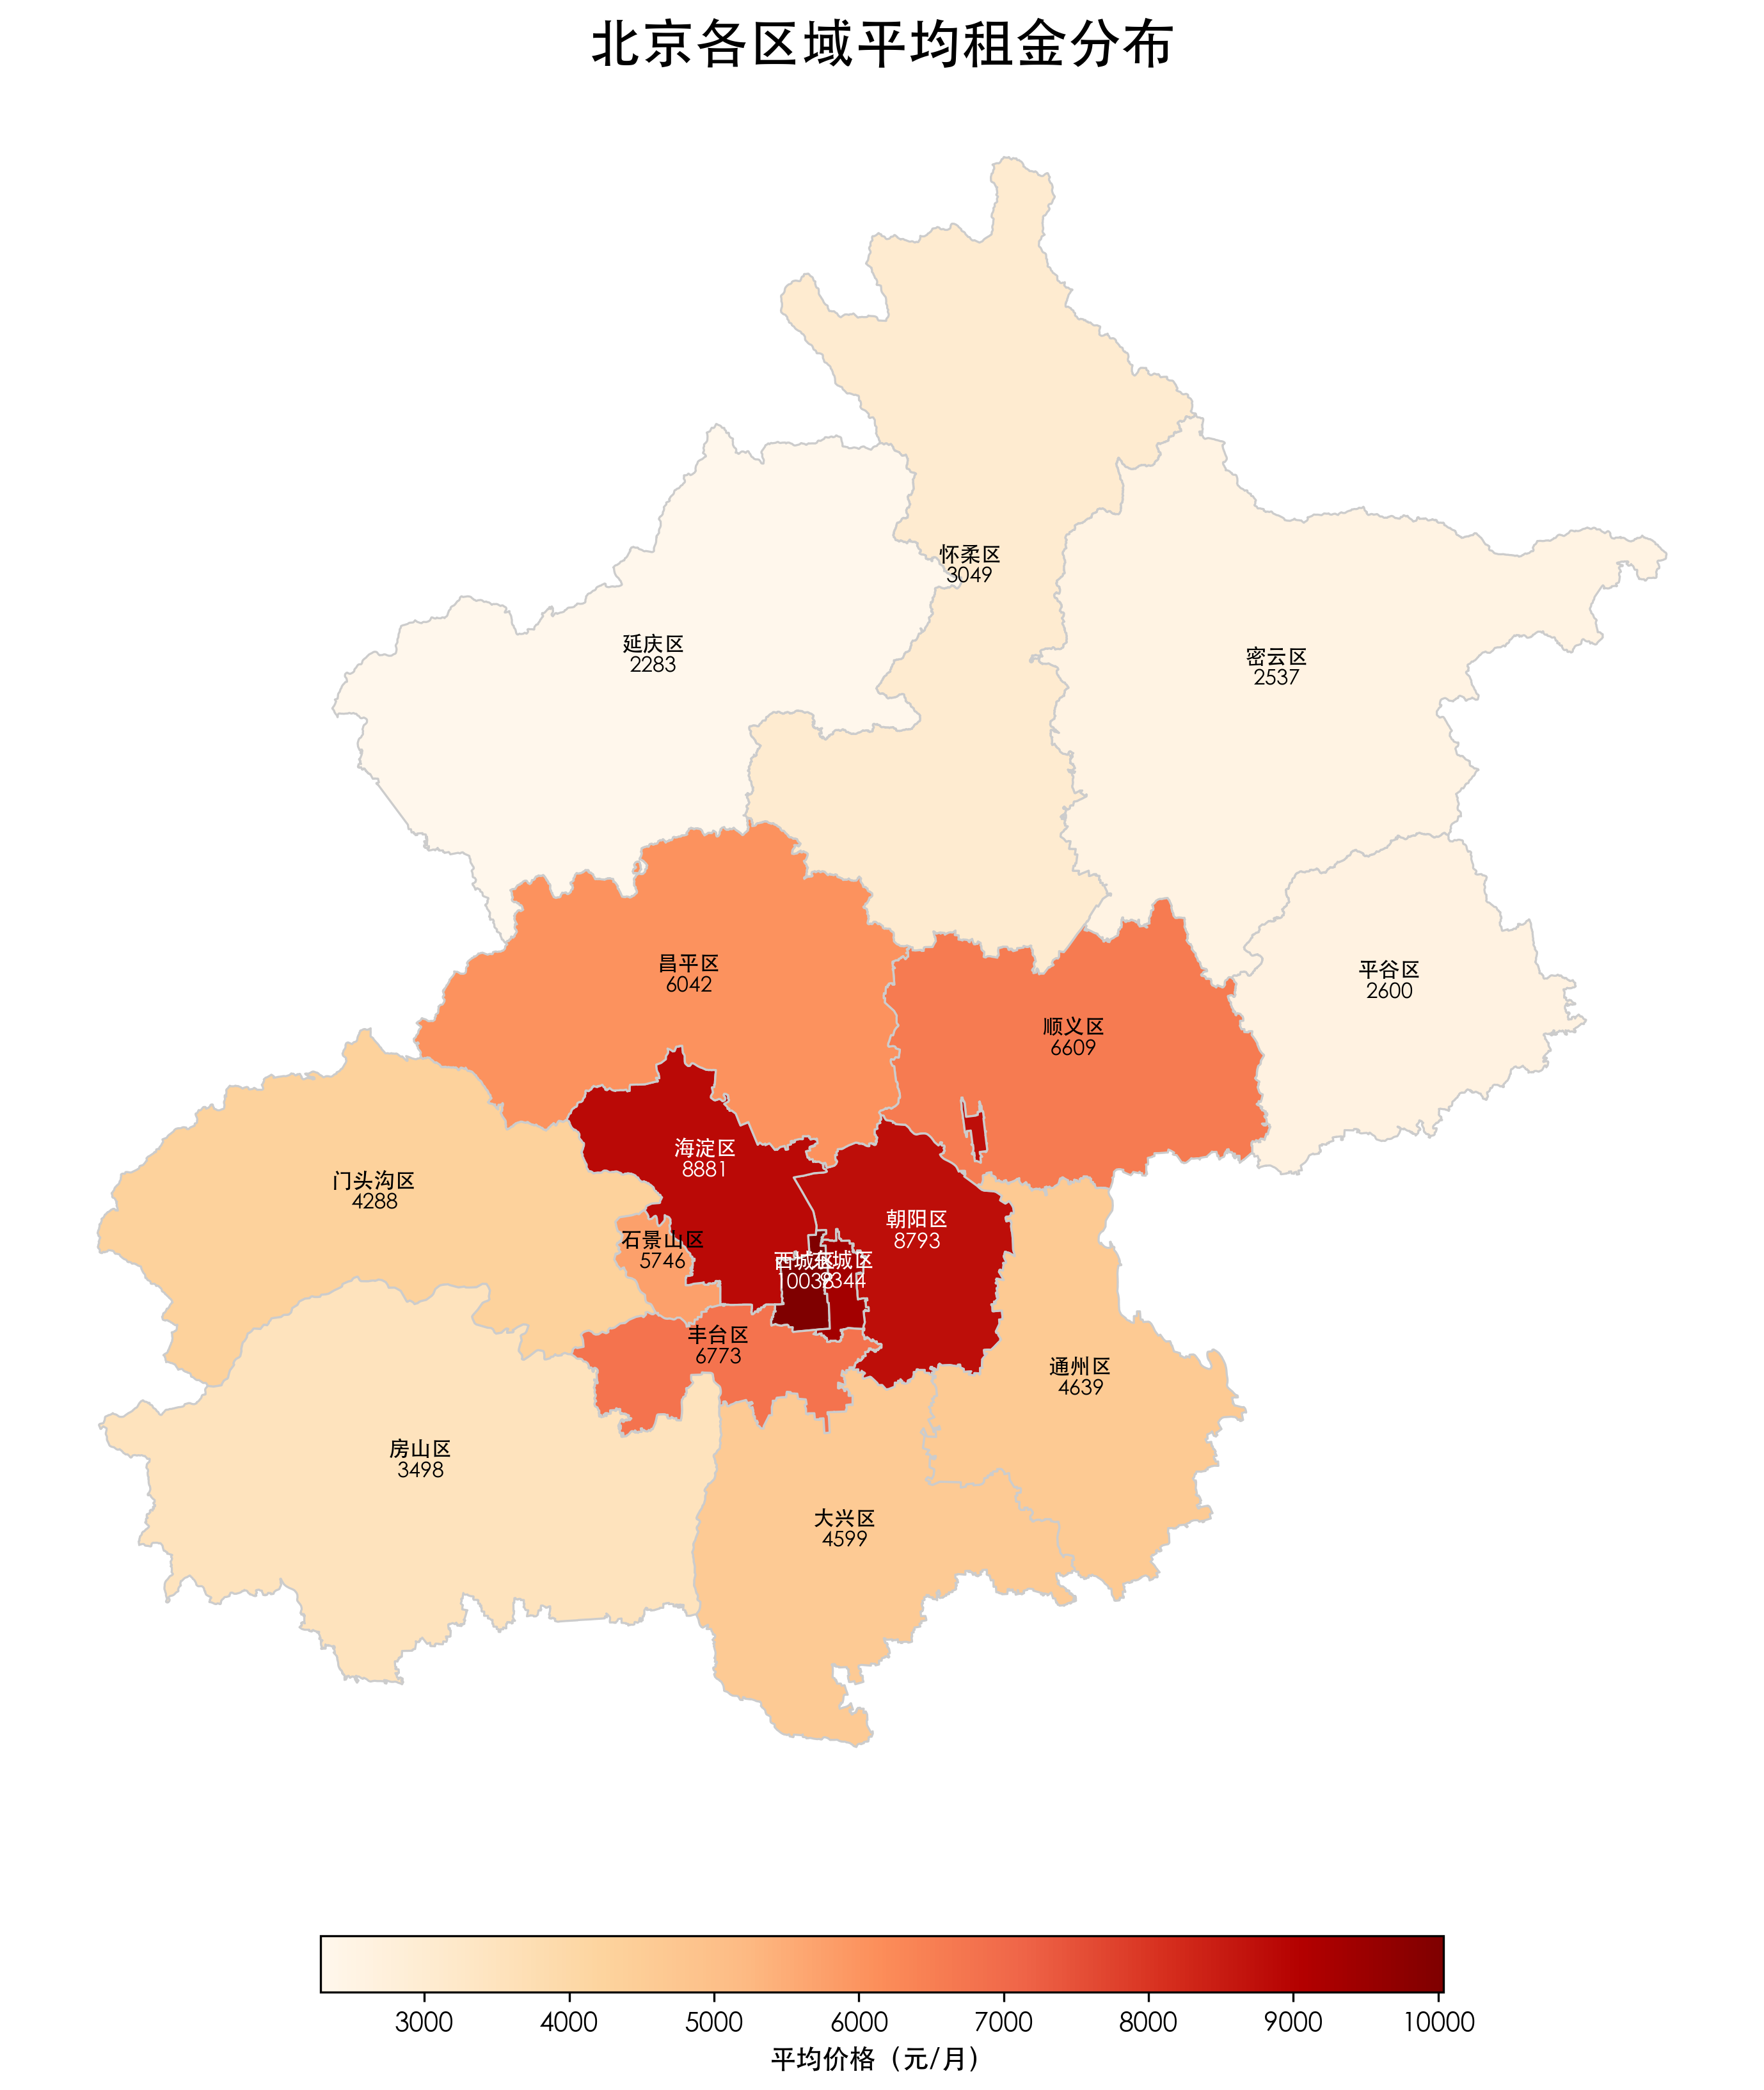
\includegraphics[width=0.7\linewidth]{../../figure/bj_region_heat_map.png}
    \caption{北京各区域平均租金分布}
    \label{fig:bj_region_heat_map}
\end{figure}
\begin{figure}[htbp]
    \centering
    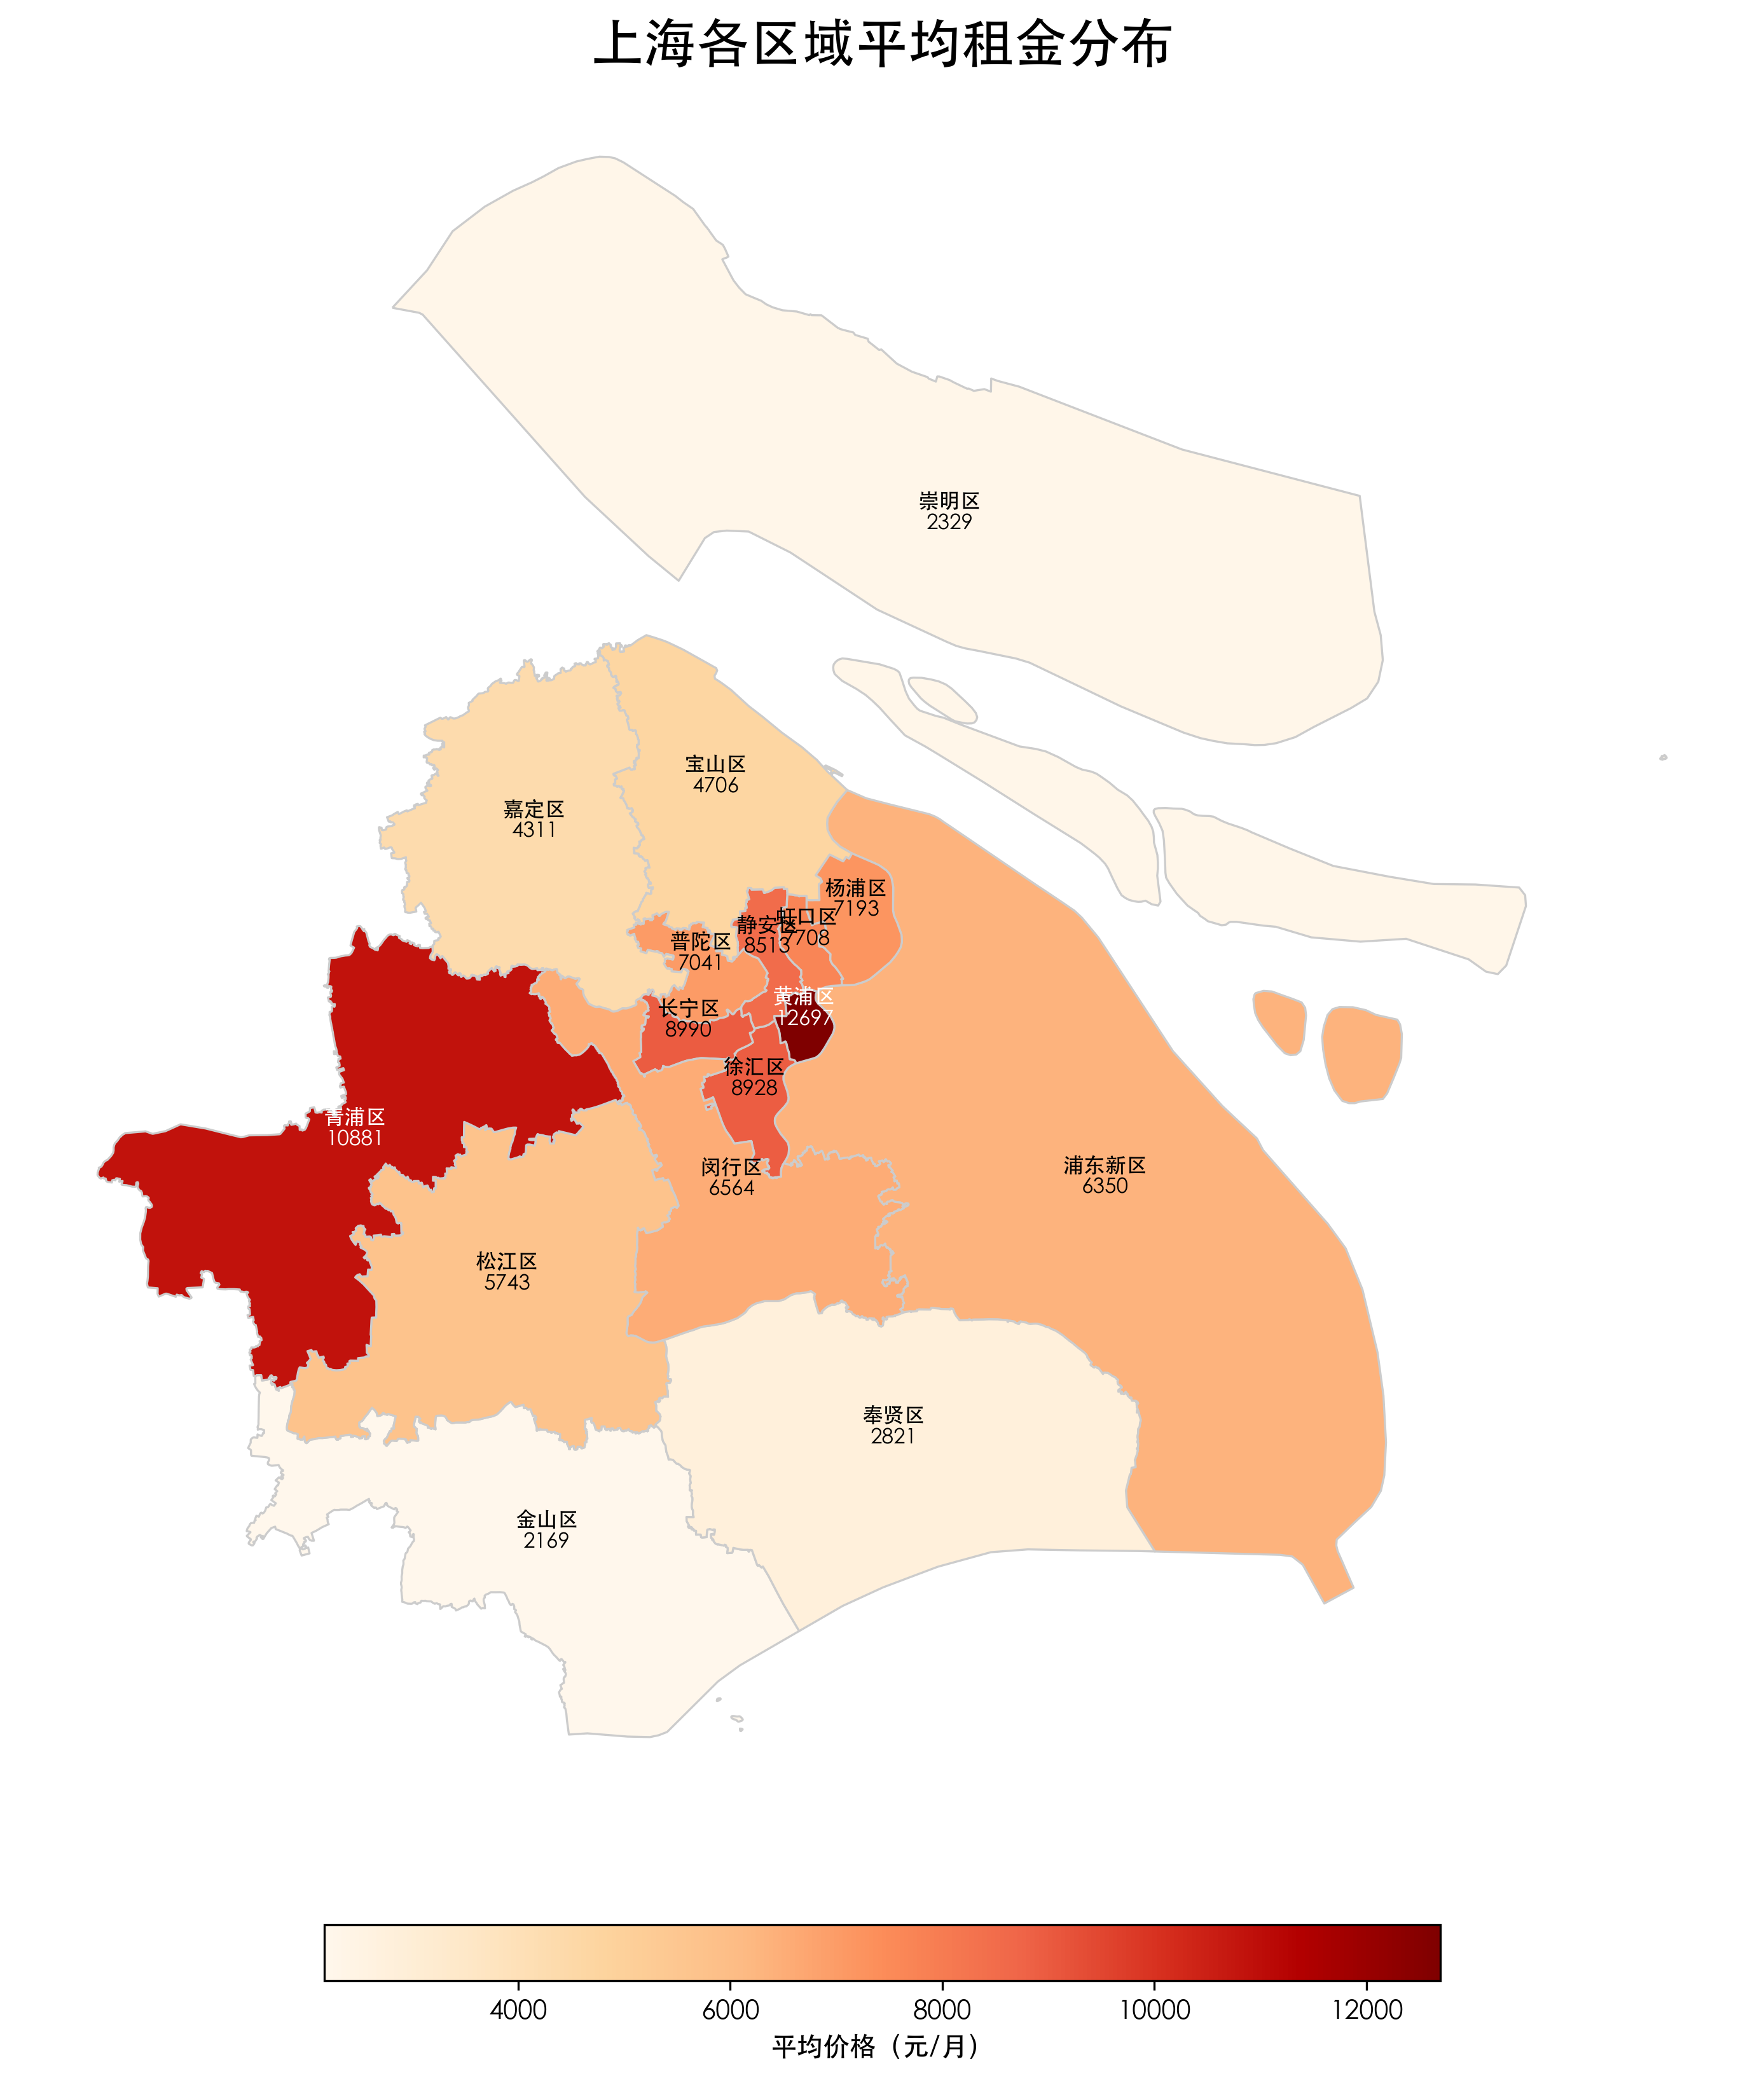
\includegraphics[width=0.7\linewidth]{../../figure/sh_region_heat_map.png}
    \caption{上海各区域平均租金分布}
    \label{fig:sh_region_heat_map}
\end{figure}
\begin{figure}[htbp]
    \centering
    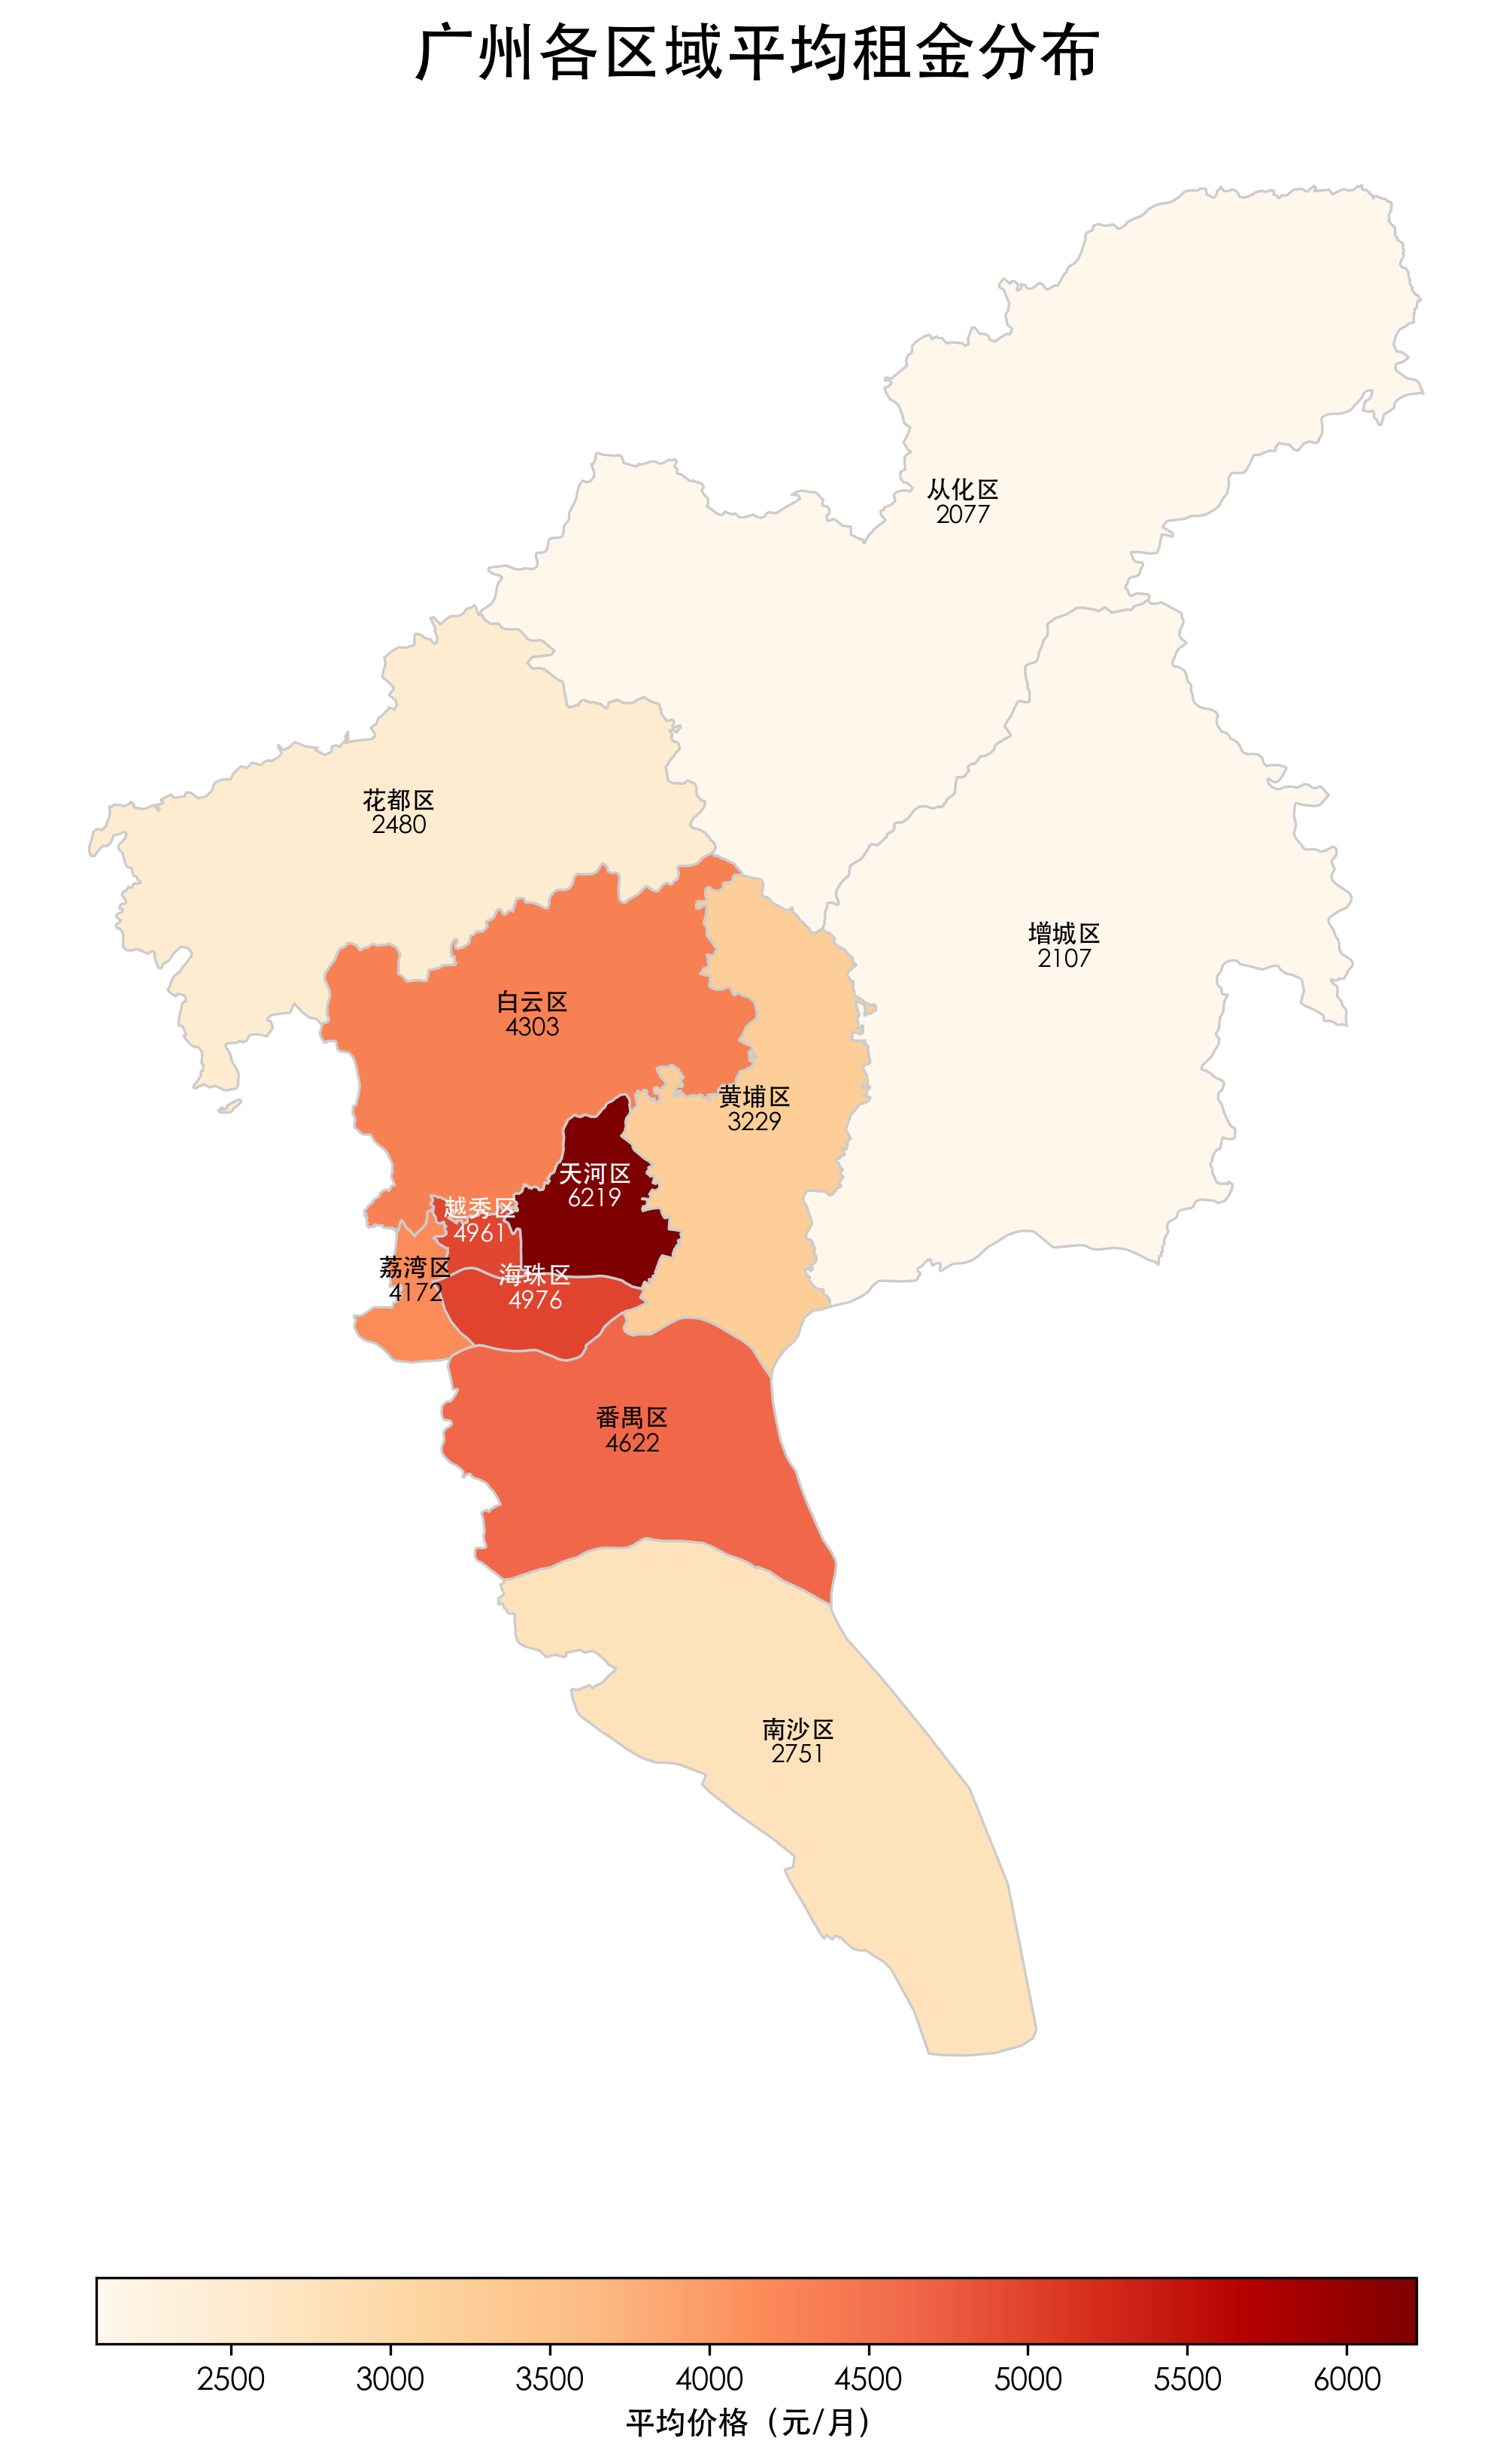
\includegraphics[width=0.7\linewidth]{../../figure/gz_region_heat_map.png}
    \caption{广州各区域平均租金分布}
    \label{fig:gz_region_heat_map}
\end{figure}
\begin{figure}[htbp]
    \centering
    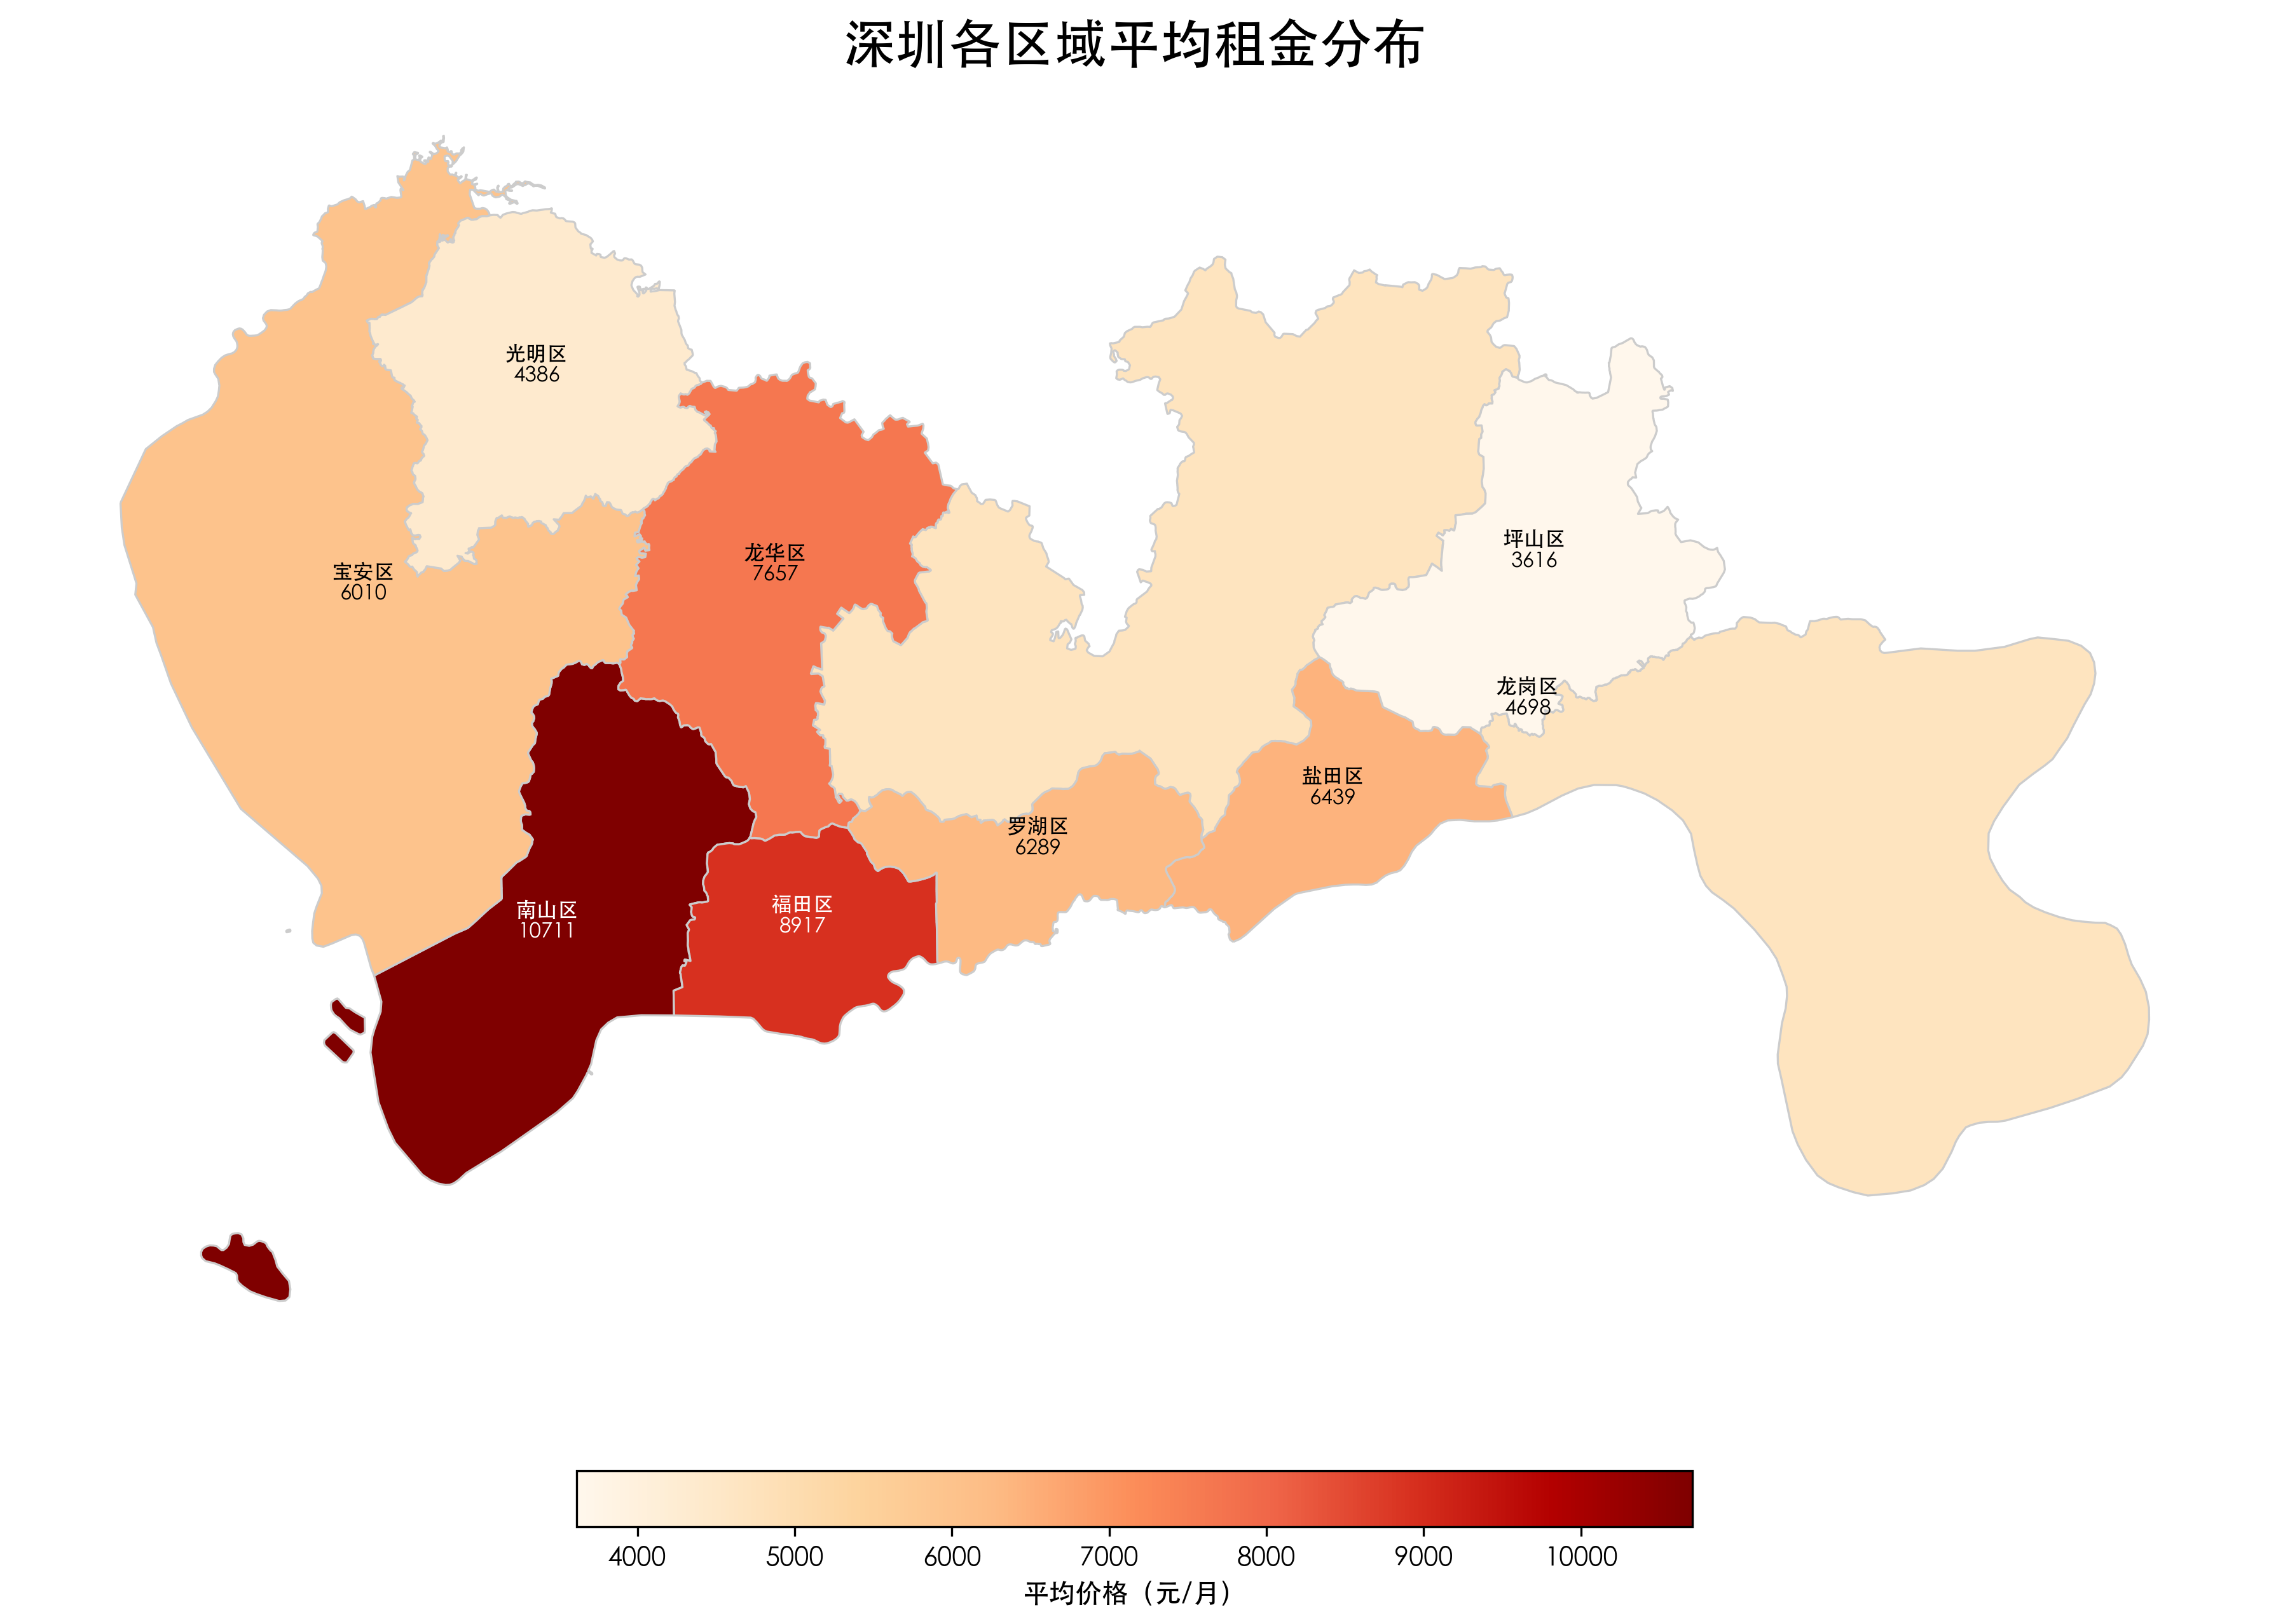
\includegraphics[width=0.7\linewidth]{../../figure/sz_region_heat_map.png}
    \caption{深圳各区域平均租金分布}
    \label{fig:sz_region_heat_map}
\end{figure}
\begin{figure}[htbp]
    \centering
    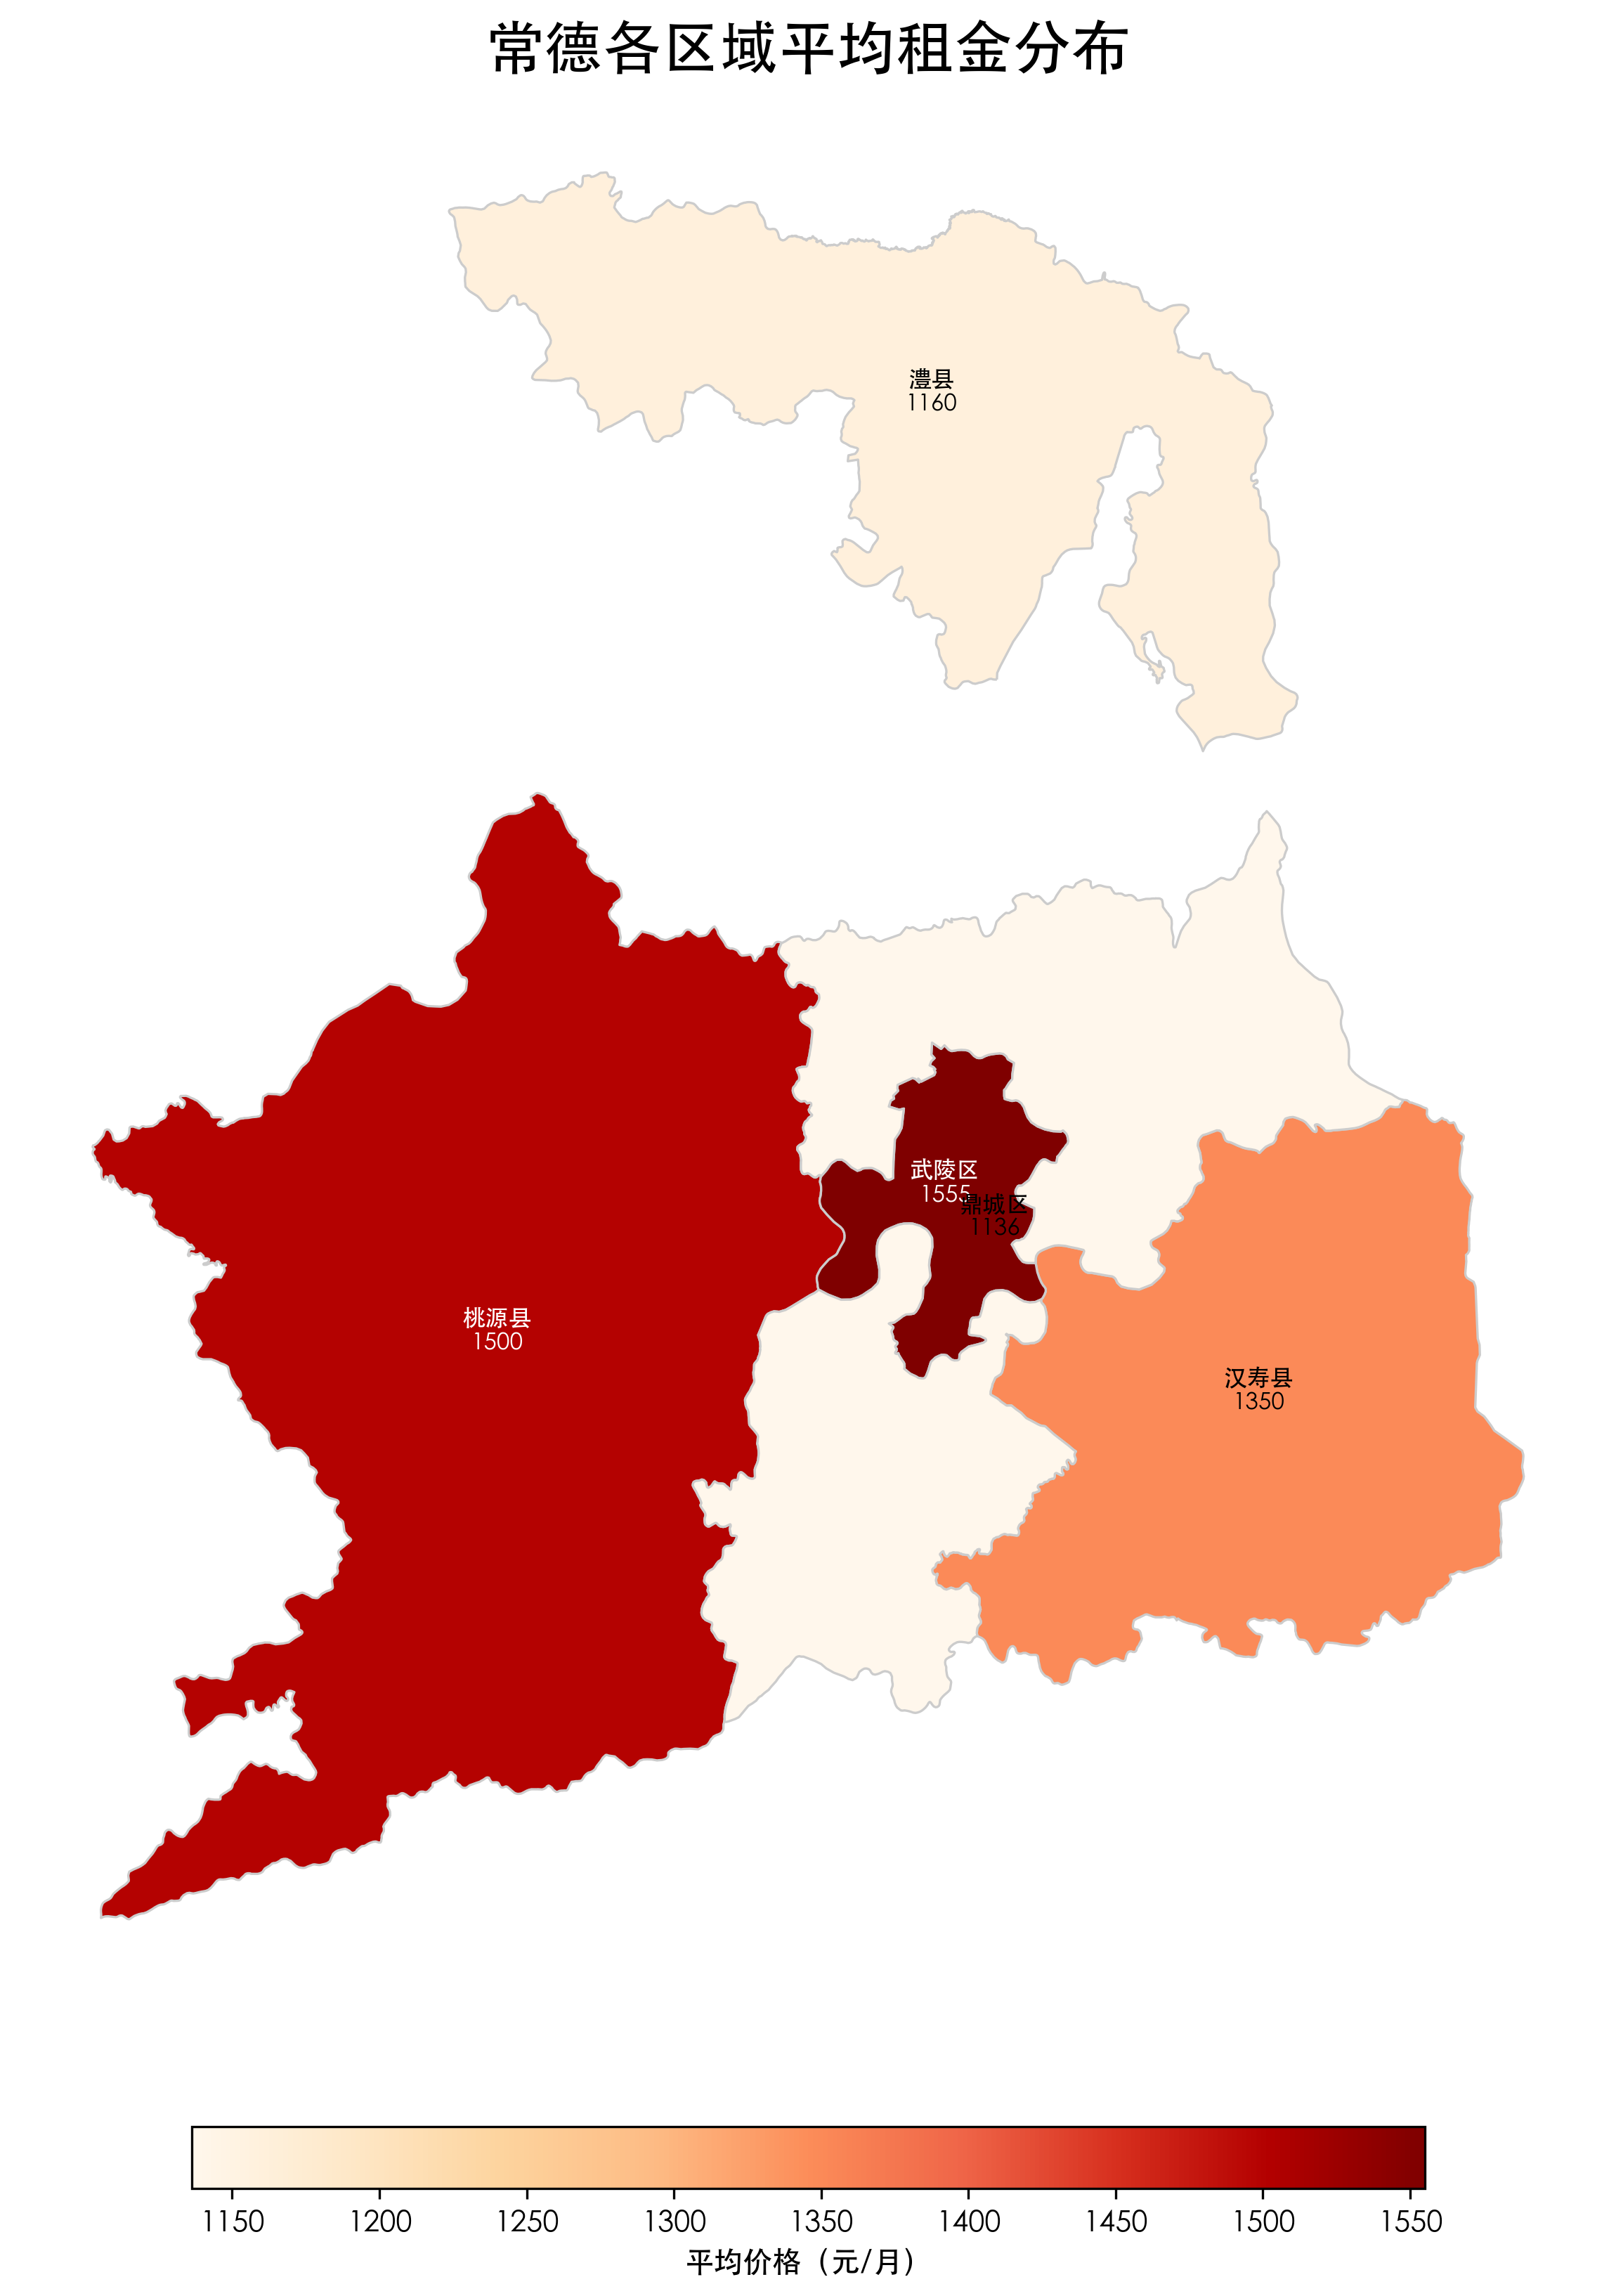
\includegraphics[width=0.7\linewidth]{../../figure/changde_region_heat_map.png}
    \caption{常德各区域平均租金分布}
    \label{fig:changde_region_heat_map}
\end{figure}

\subsection{朝向分析}
为了观察价格分布,画出各城市各朝向的价格概率分布曲线,由于画分布图时,会受到极端大值的影响,使得图像不直观,于是筛除了大于平均值加上2倍标准差的数据,使得图像更加清晰明了。如图~\ref{fig:bj_direction_unit_price_distribution}、图~\ref{fig:sh_direction_unit_price_distribution}、图~\ref{fig:gz_direction_unit_price_distribution}、图~\ref{fig:sz_direction_unit_price_distribution}、图~\ref{fig:changde_direction_unit_price_distribution}。
\begin{figure}[htbp]
    \centering
    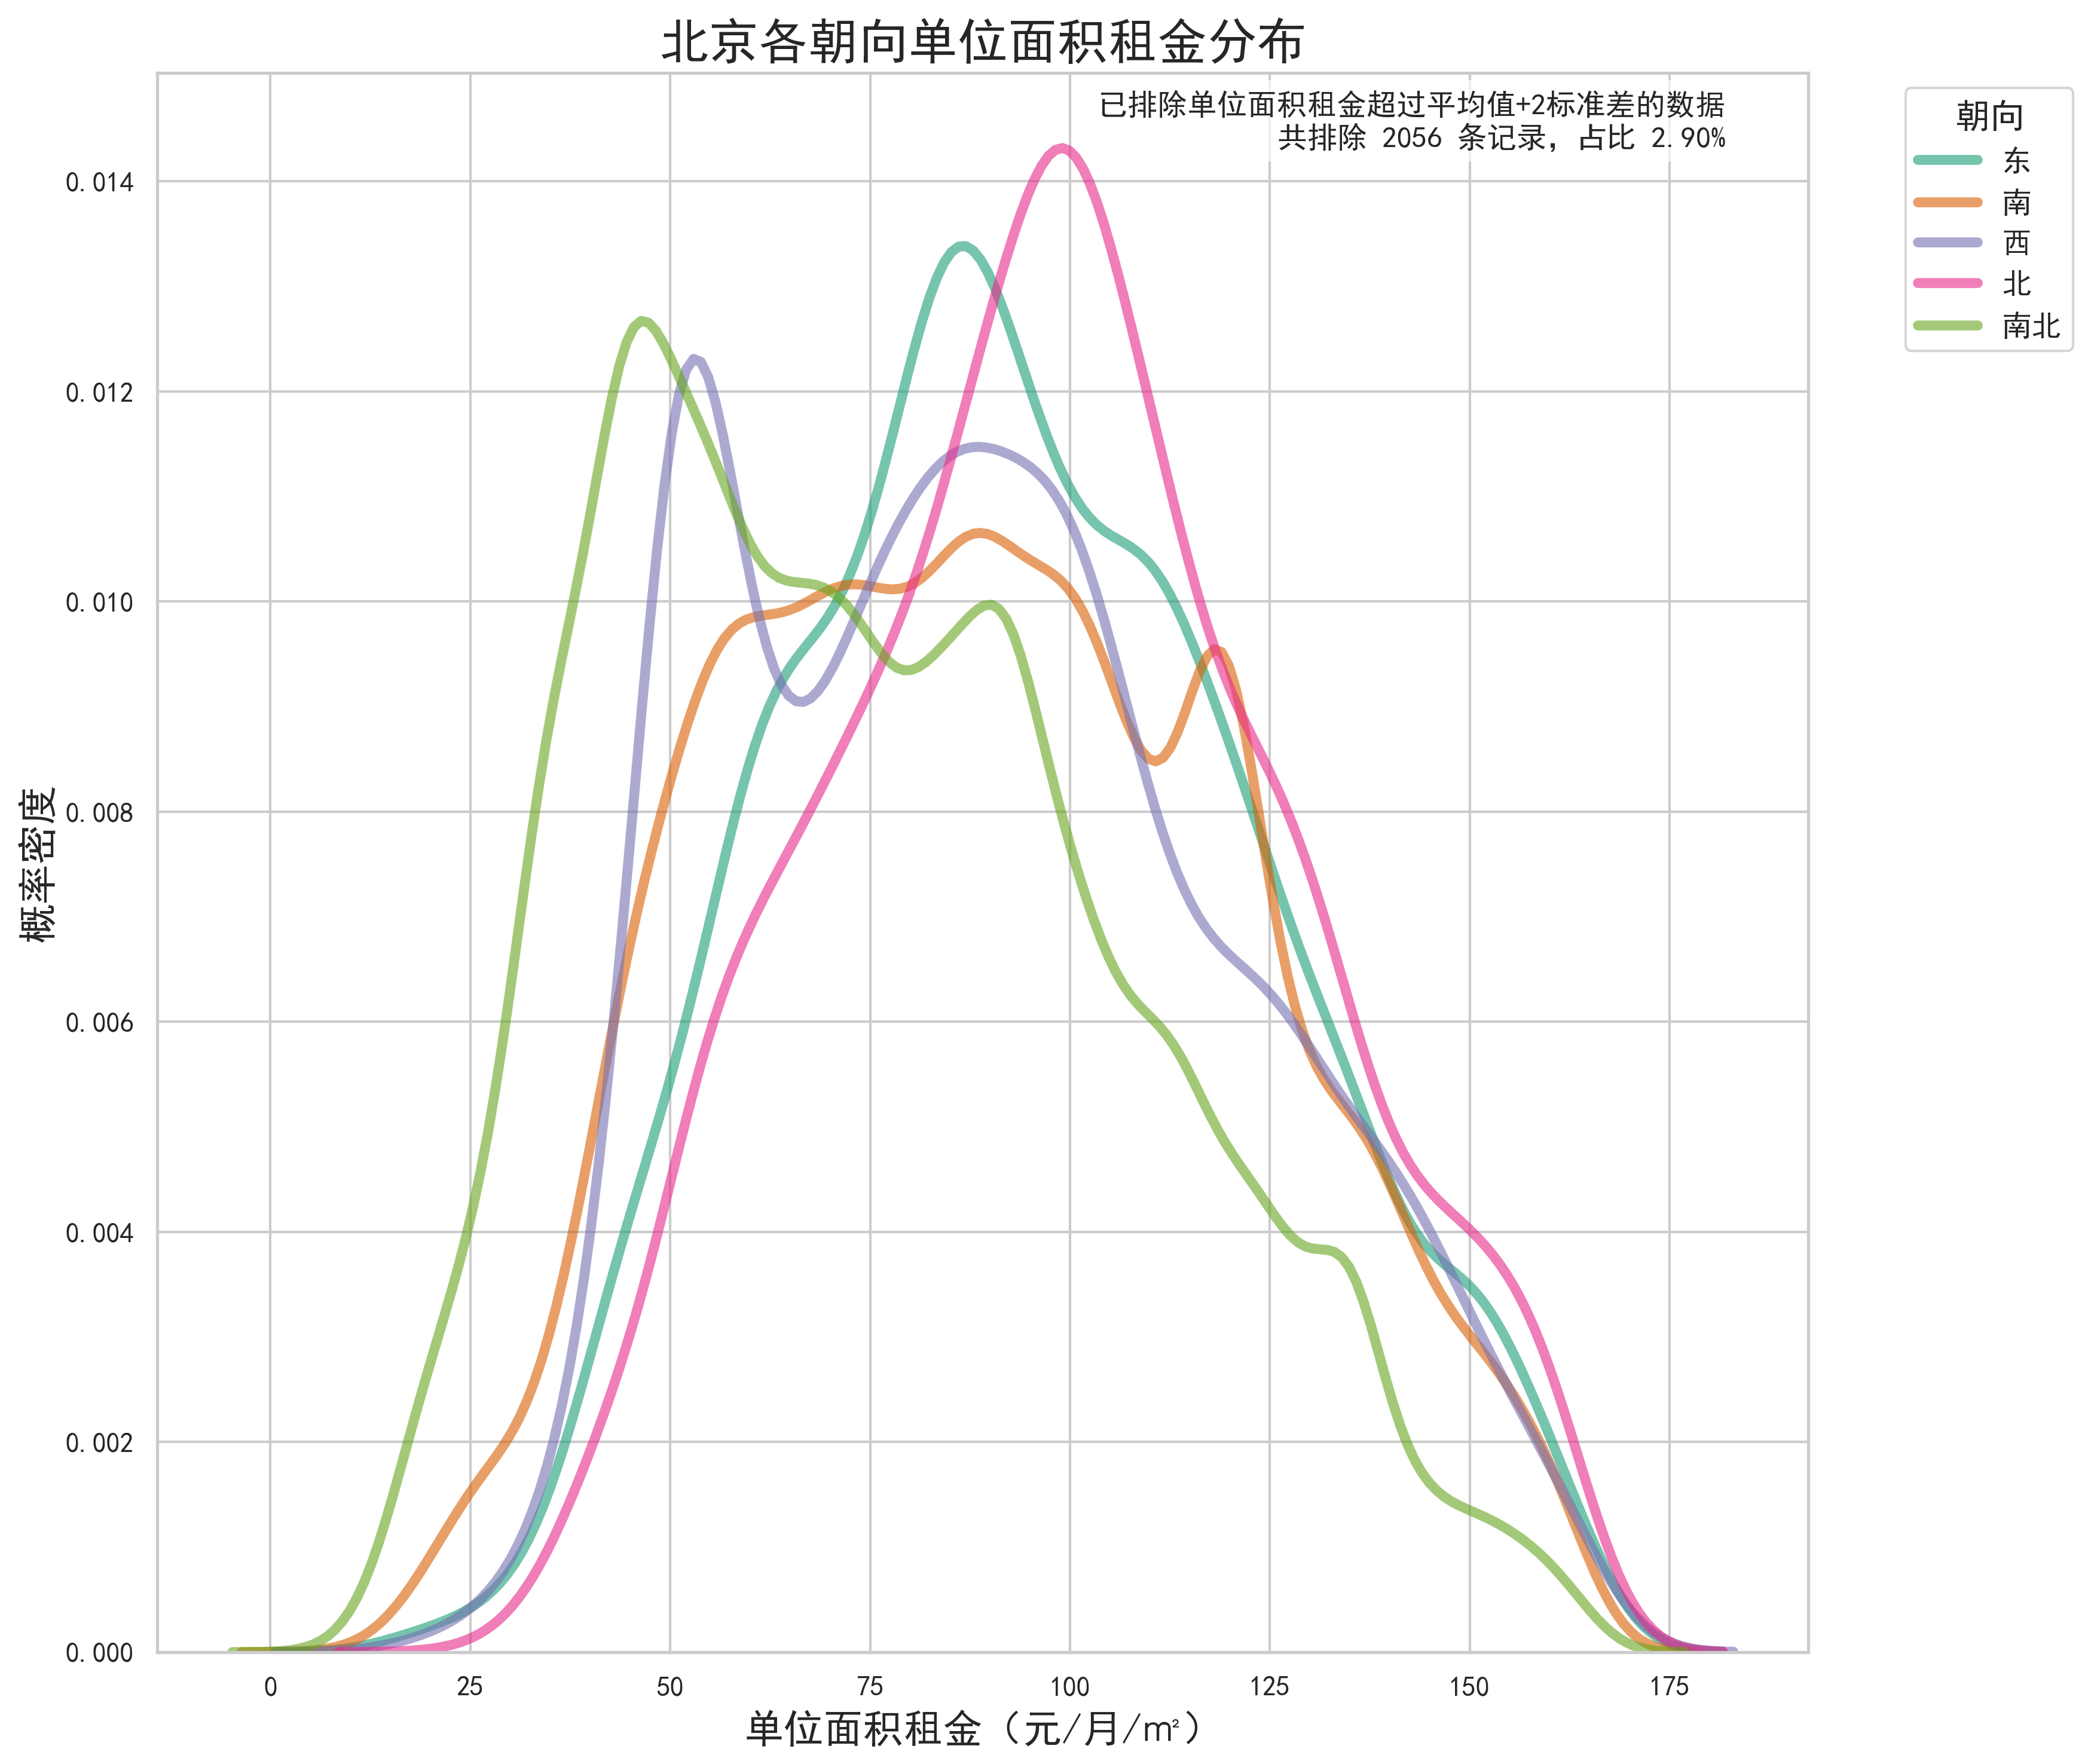
\includegraphics[width=0.7\linewidth]{../../figure/bj_direction_unit_price_distribution.png}
    \caption{北京各区域平均租金分布}
    \label{fig:bj_direction_unit_price_distribution}
\end{figure}
\begin{figure}[htbp]
    \centering
    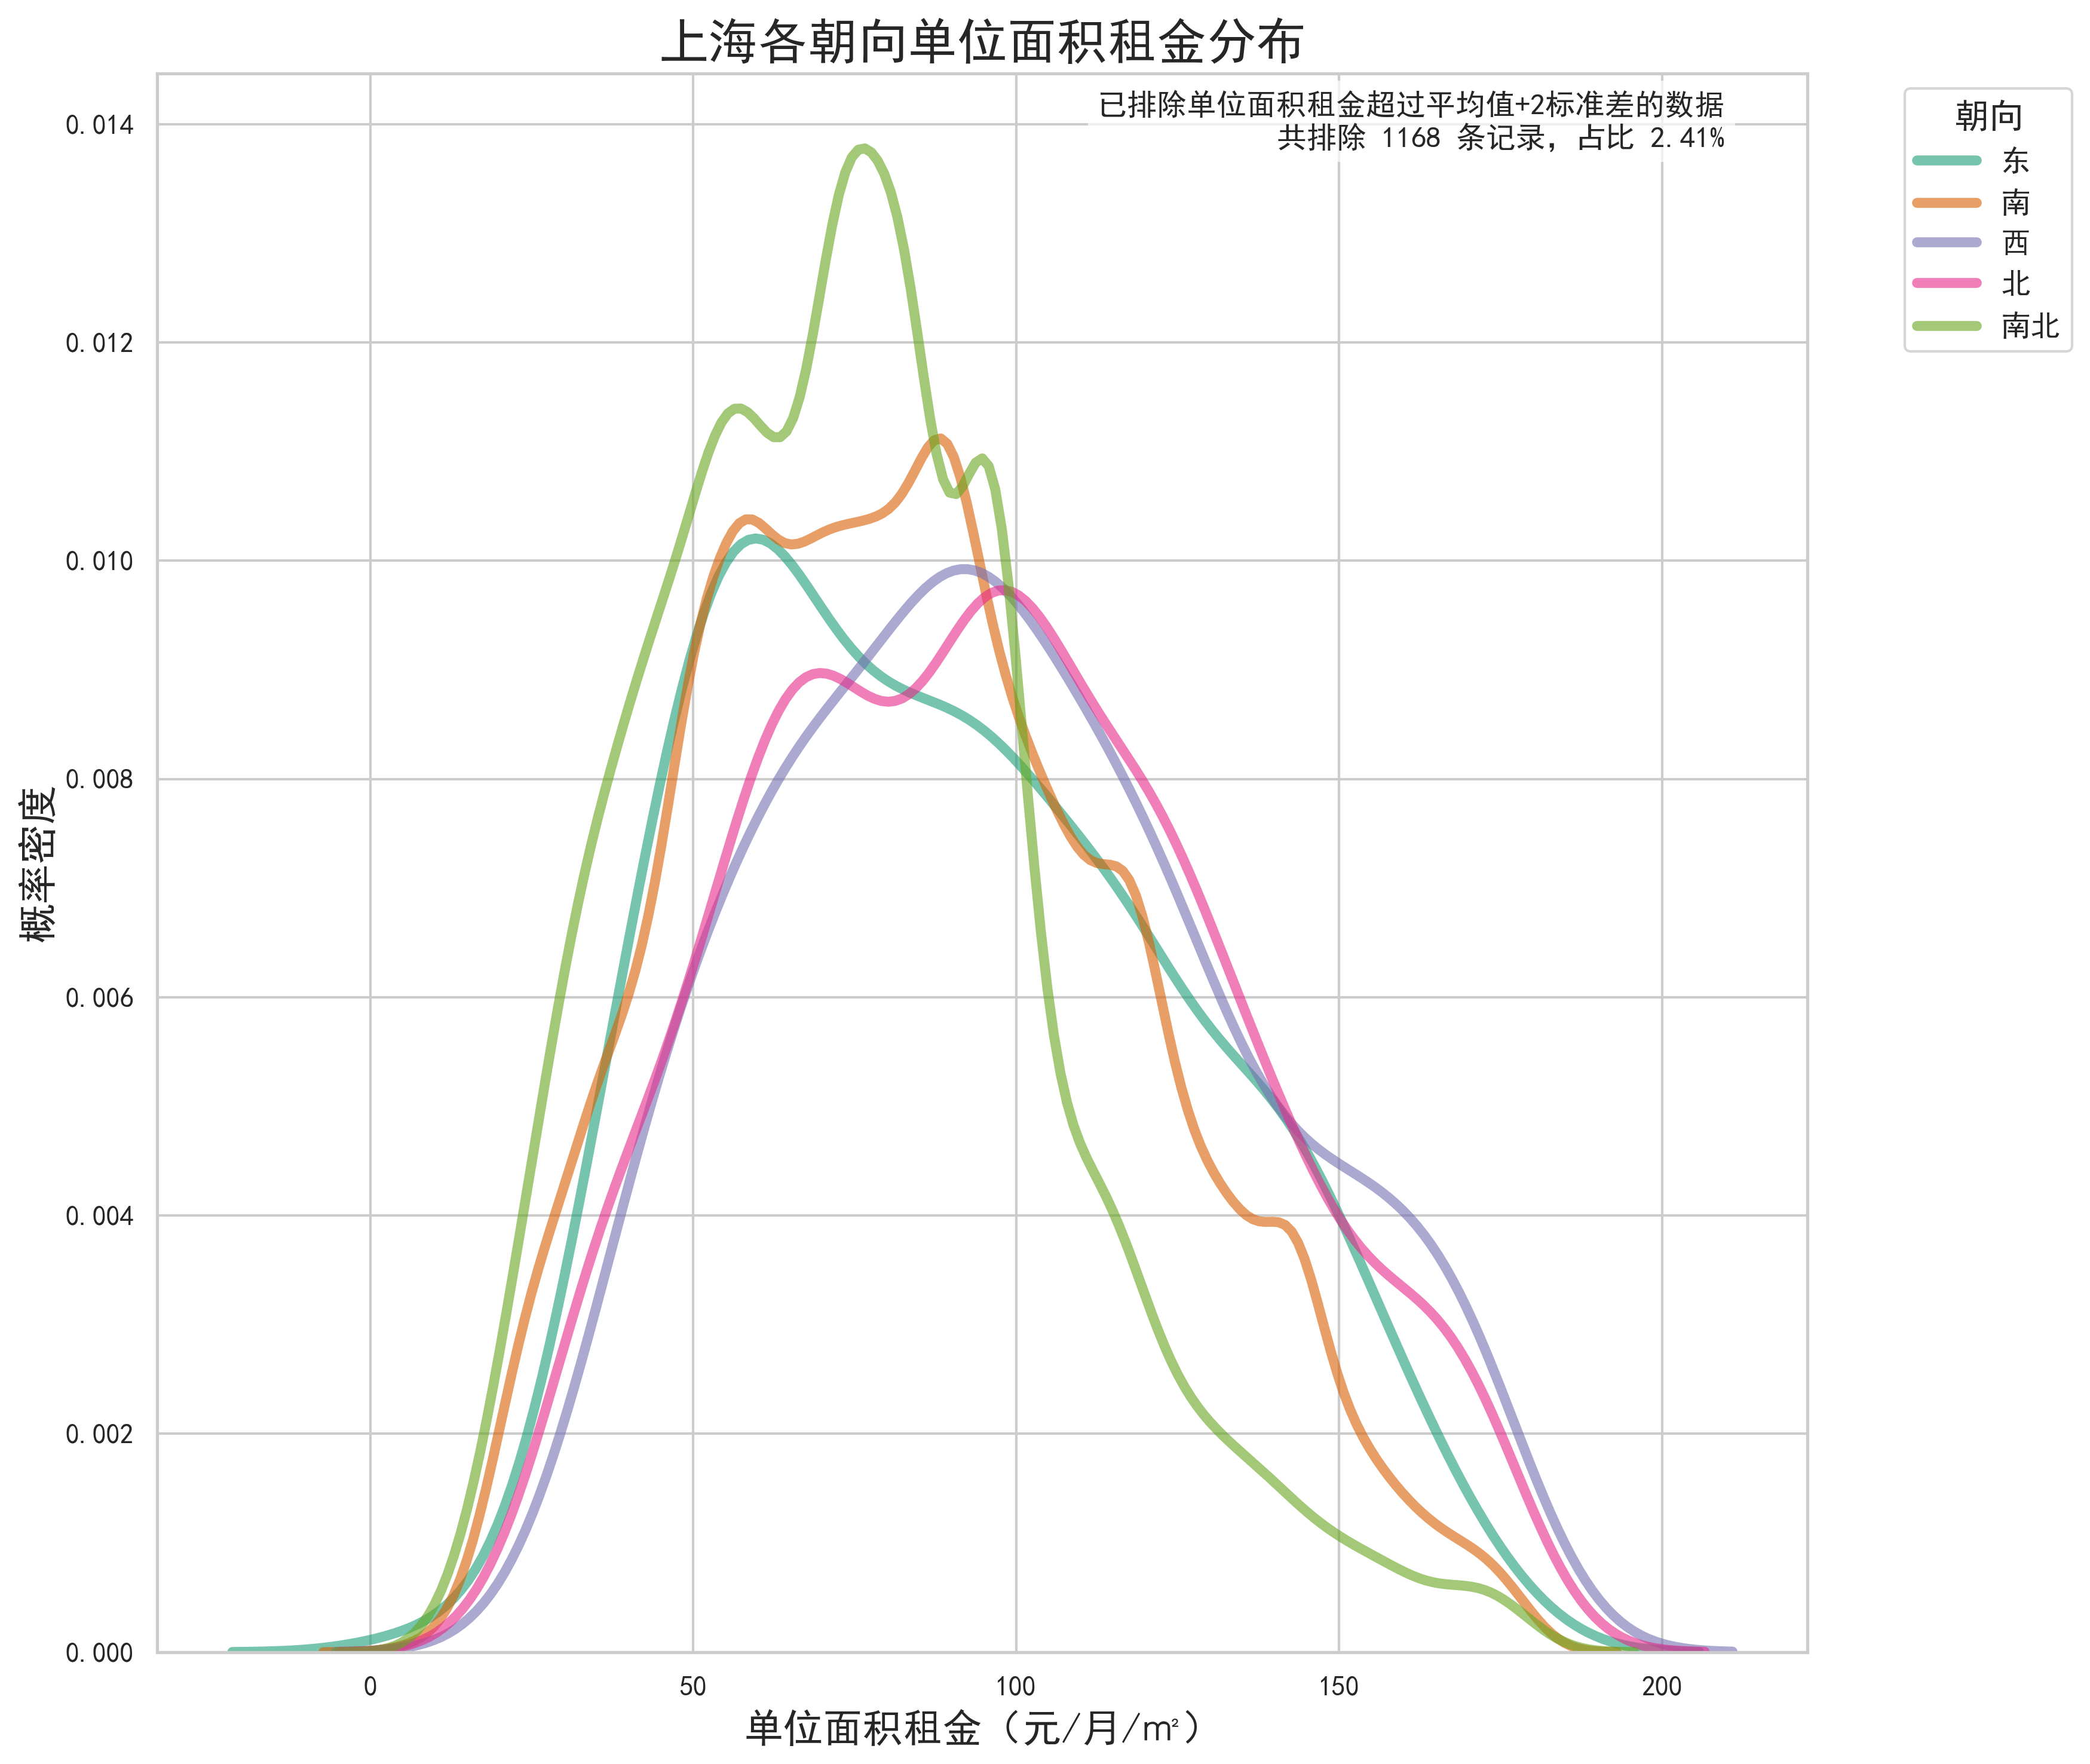
\includegraphics[width=0.7\linewidth]{../../figure/sh_direction_unit_price_distribution.png}
    \caption{上海各区域平均租金分布}
    \label{fig:sh_direction_unit_price_distribution}
\end{figure}
\begin{figure}[htbp]
    \centering
    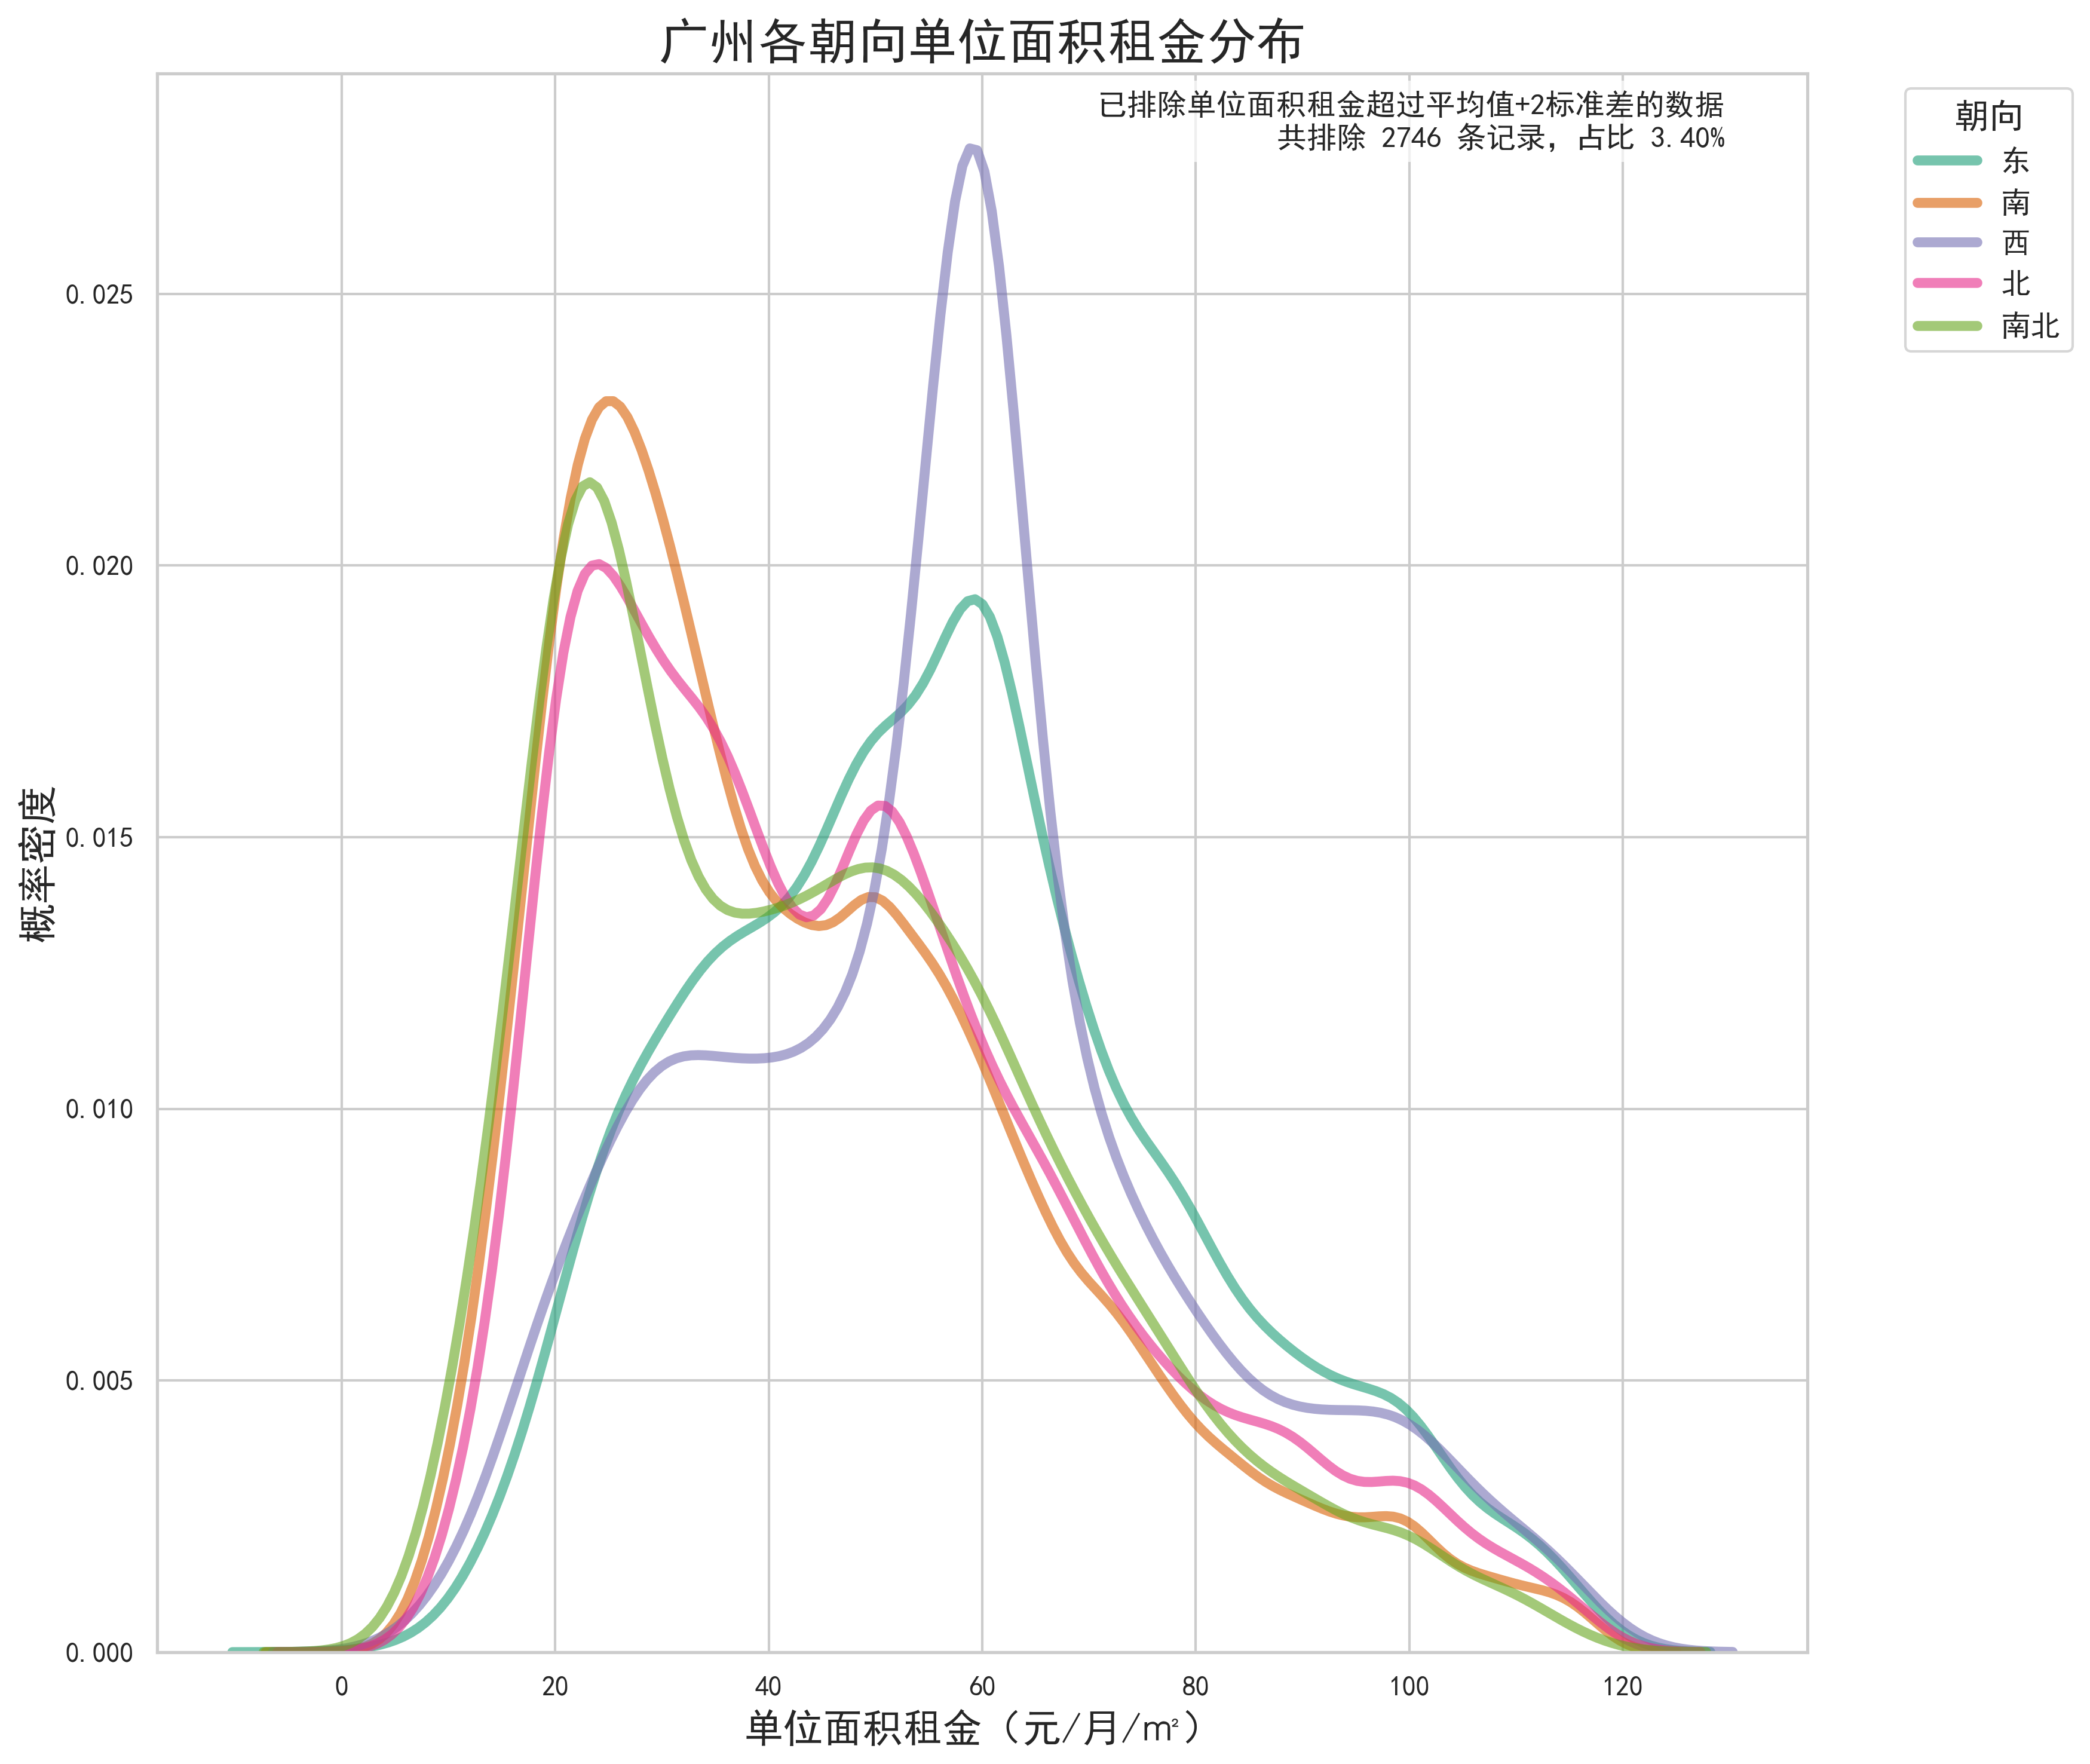
\includegraphics[width=0.7\linewidth]{../../figure/gz_direction_unit_price_distribution.png}
    \caption{广州各区域平均租金分布}
    \label{fig:gz_direction_unit_price_distribution}
\end{figure}
\begin{figure}[htbp]
    \centering
    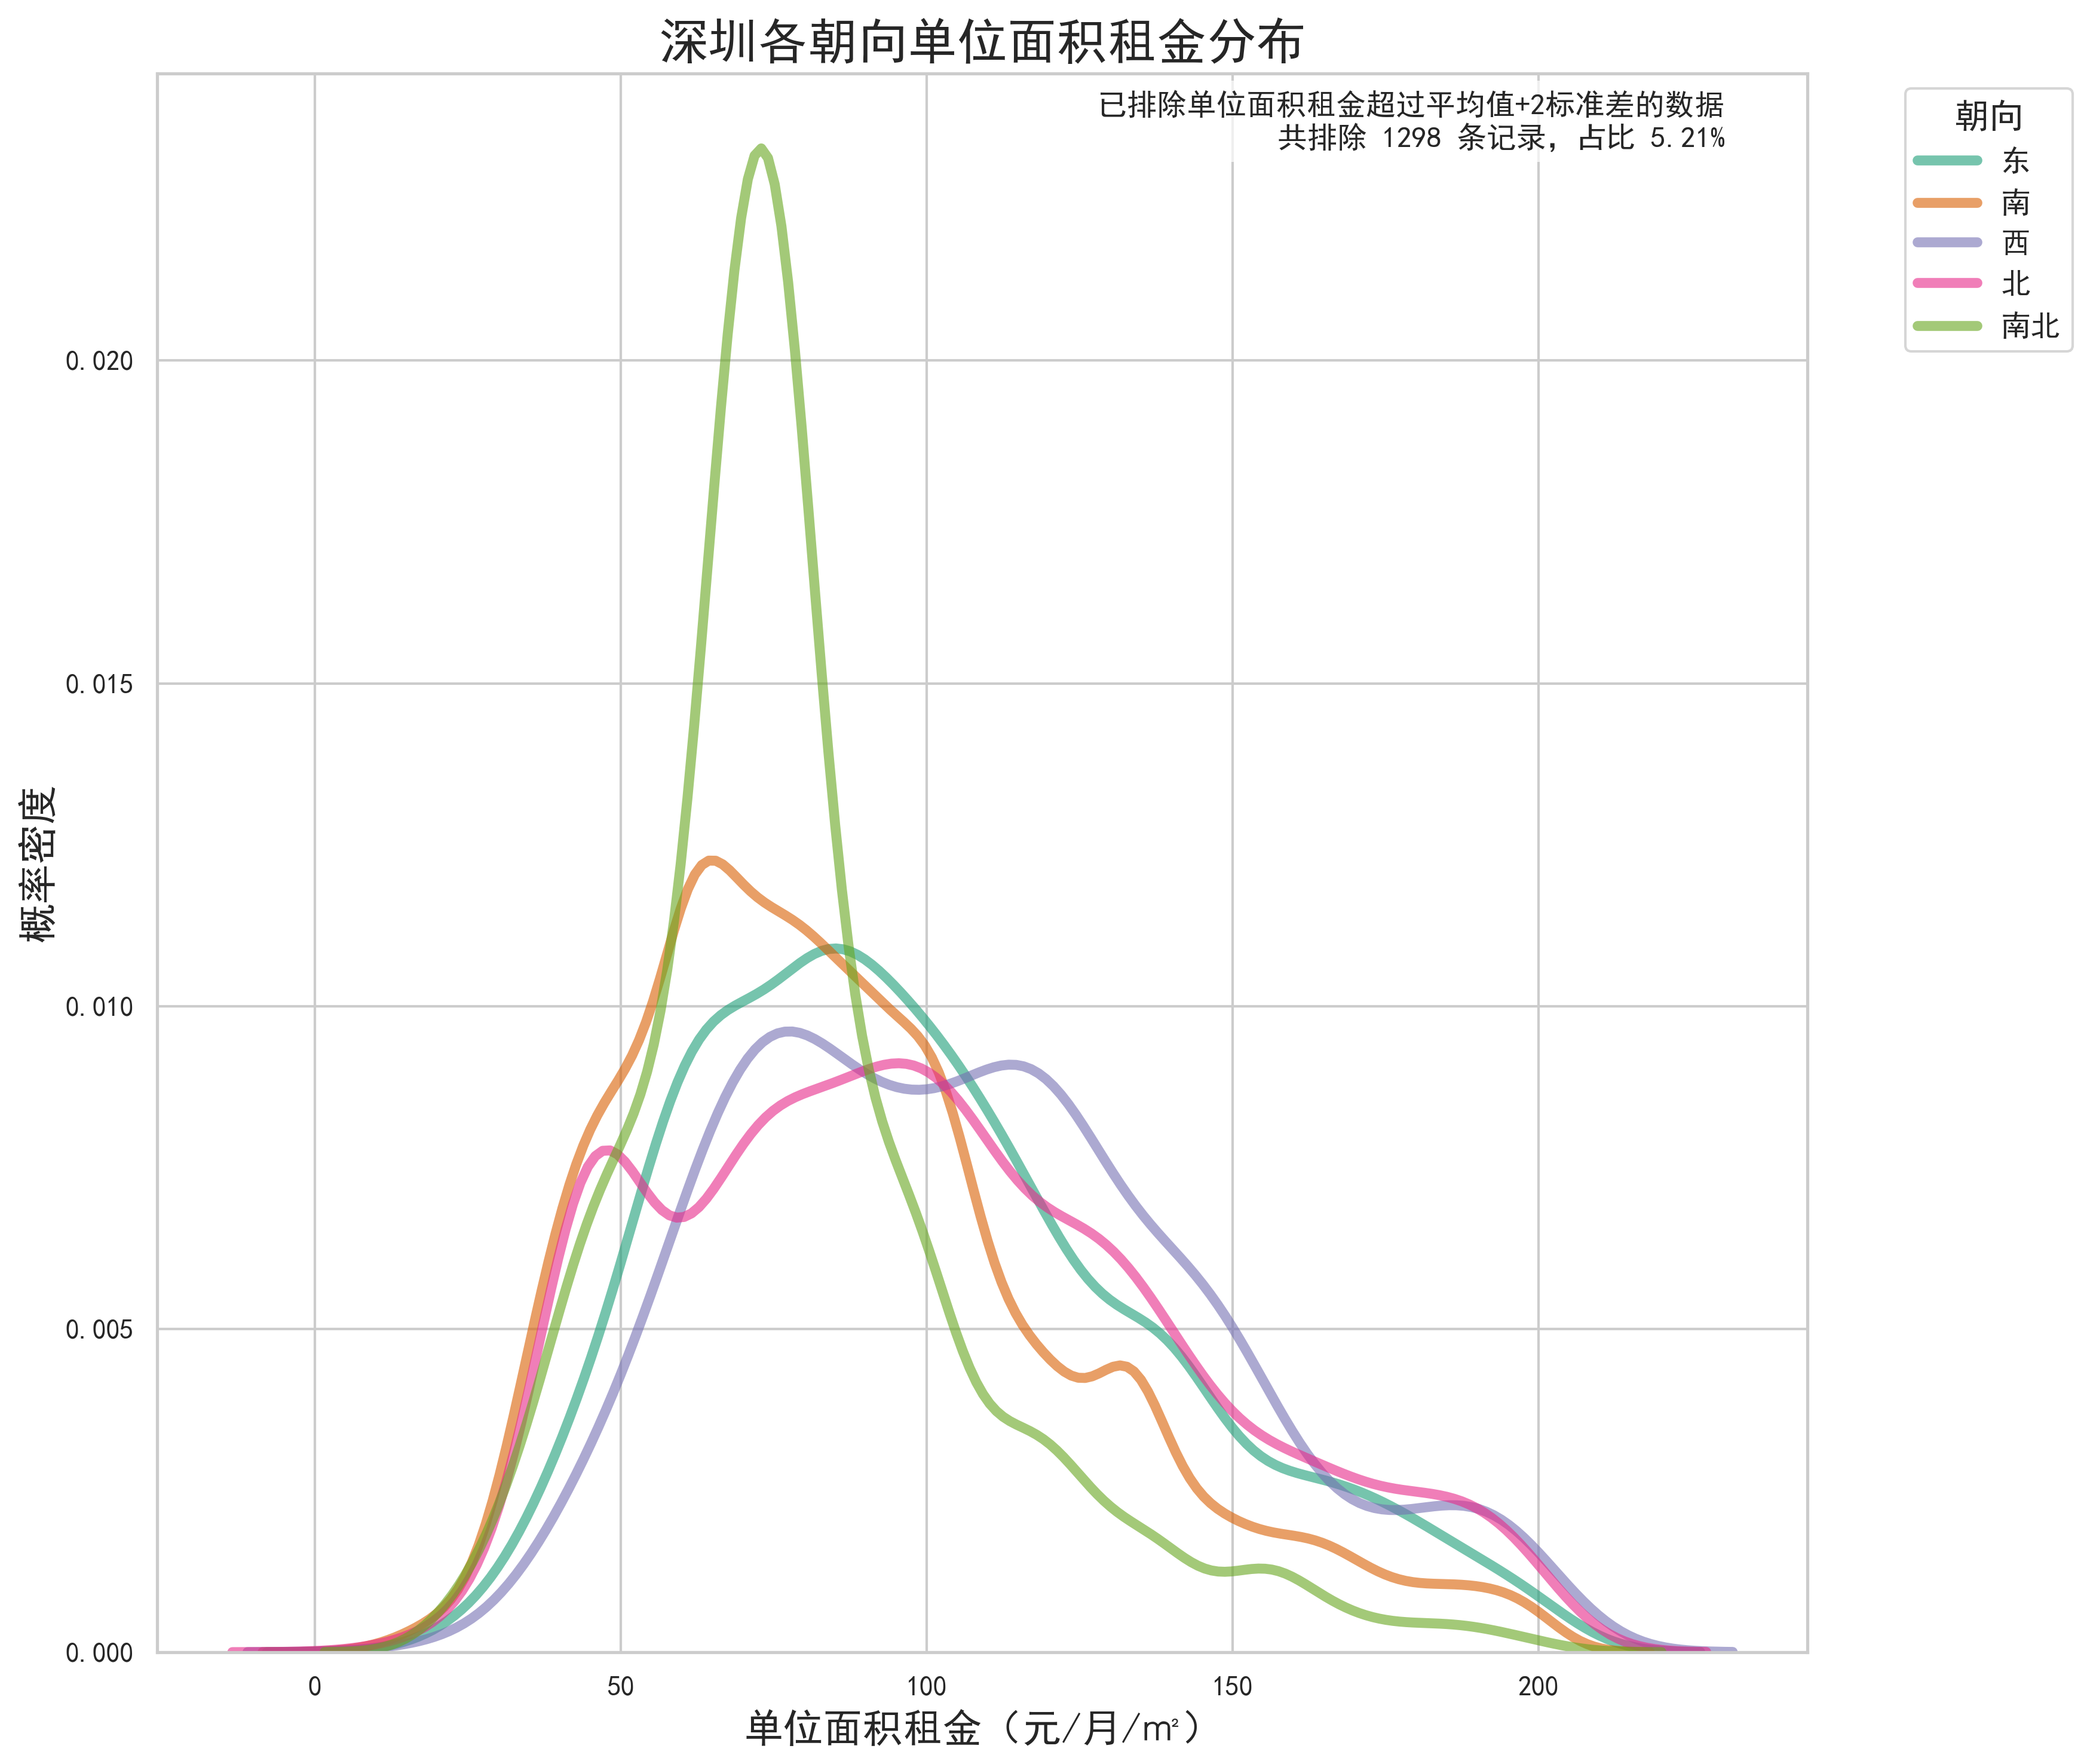
\includegraphics[width=0.7\linewidth]{../../figure/sz_direction_unit_price_distribution.png}
    \caption{深圳各区域平均租金分布}
    \label{fig:sz_direction_unit_price_distribution}
\end{figure}
\begin{figure}[htbp]
    \centering
    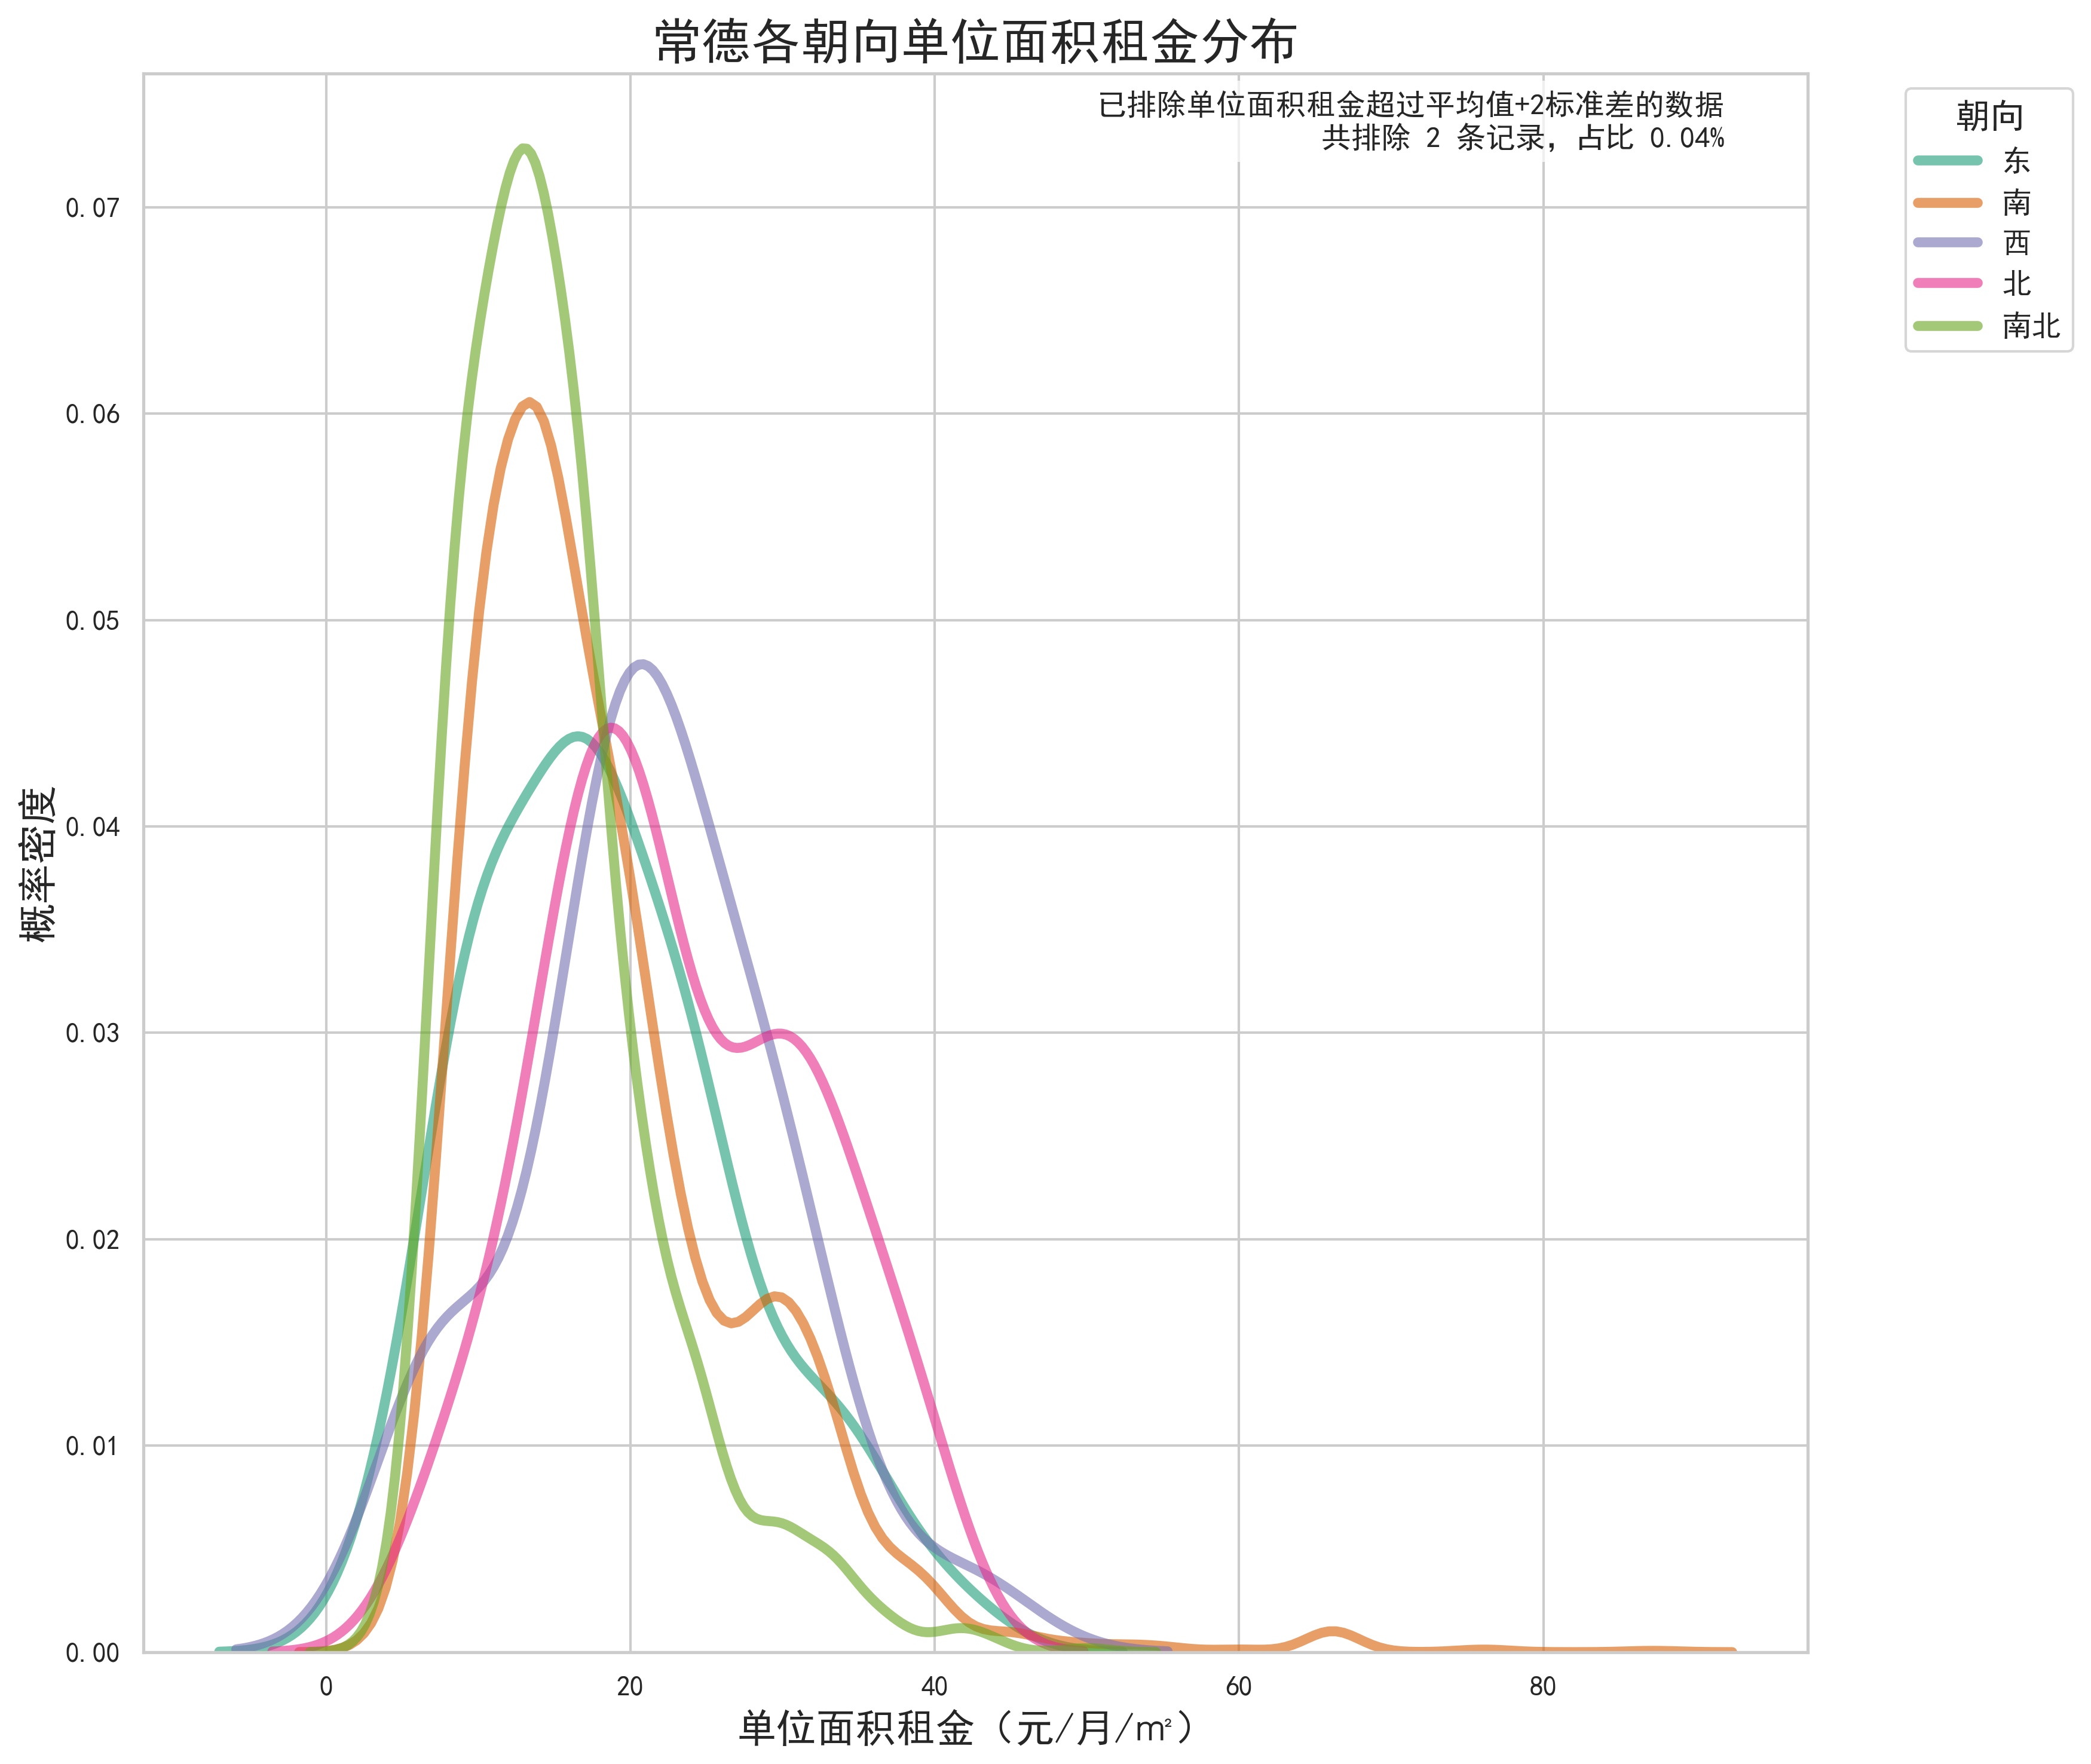
\includegraphics[width=0.7\linewidth]{../../figure/changde_direction_unit_price_distribution.png}
    \caption{常德各区域平均租金分布}
    \label{fig:changde_direction_unit_price_distribution}
\end{figure}

为了便于分析和比较大小,采用直方图对平均值进行展示,如图~\ref{fig:direction_unit_price_bar_chart}。
\begin{figure}[htbp]
    \centering
    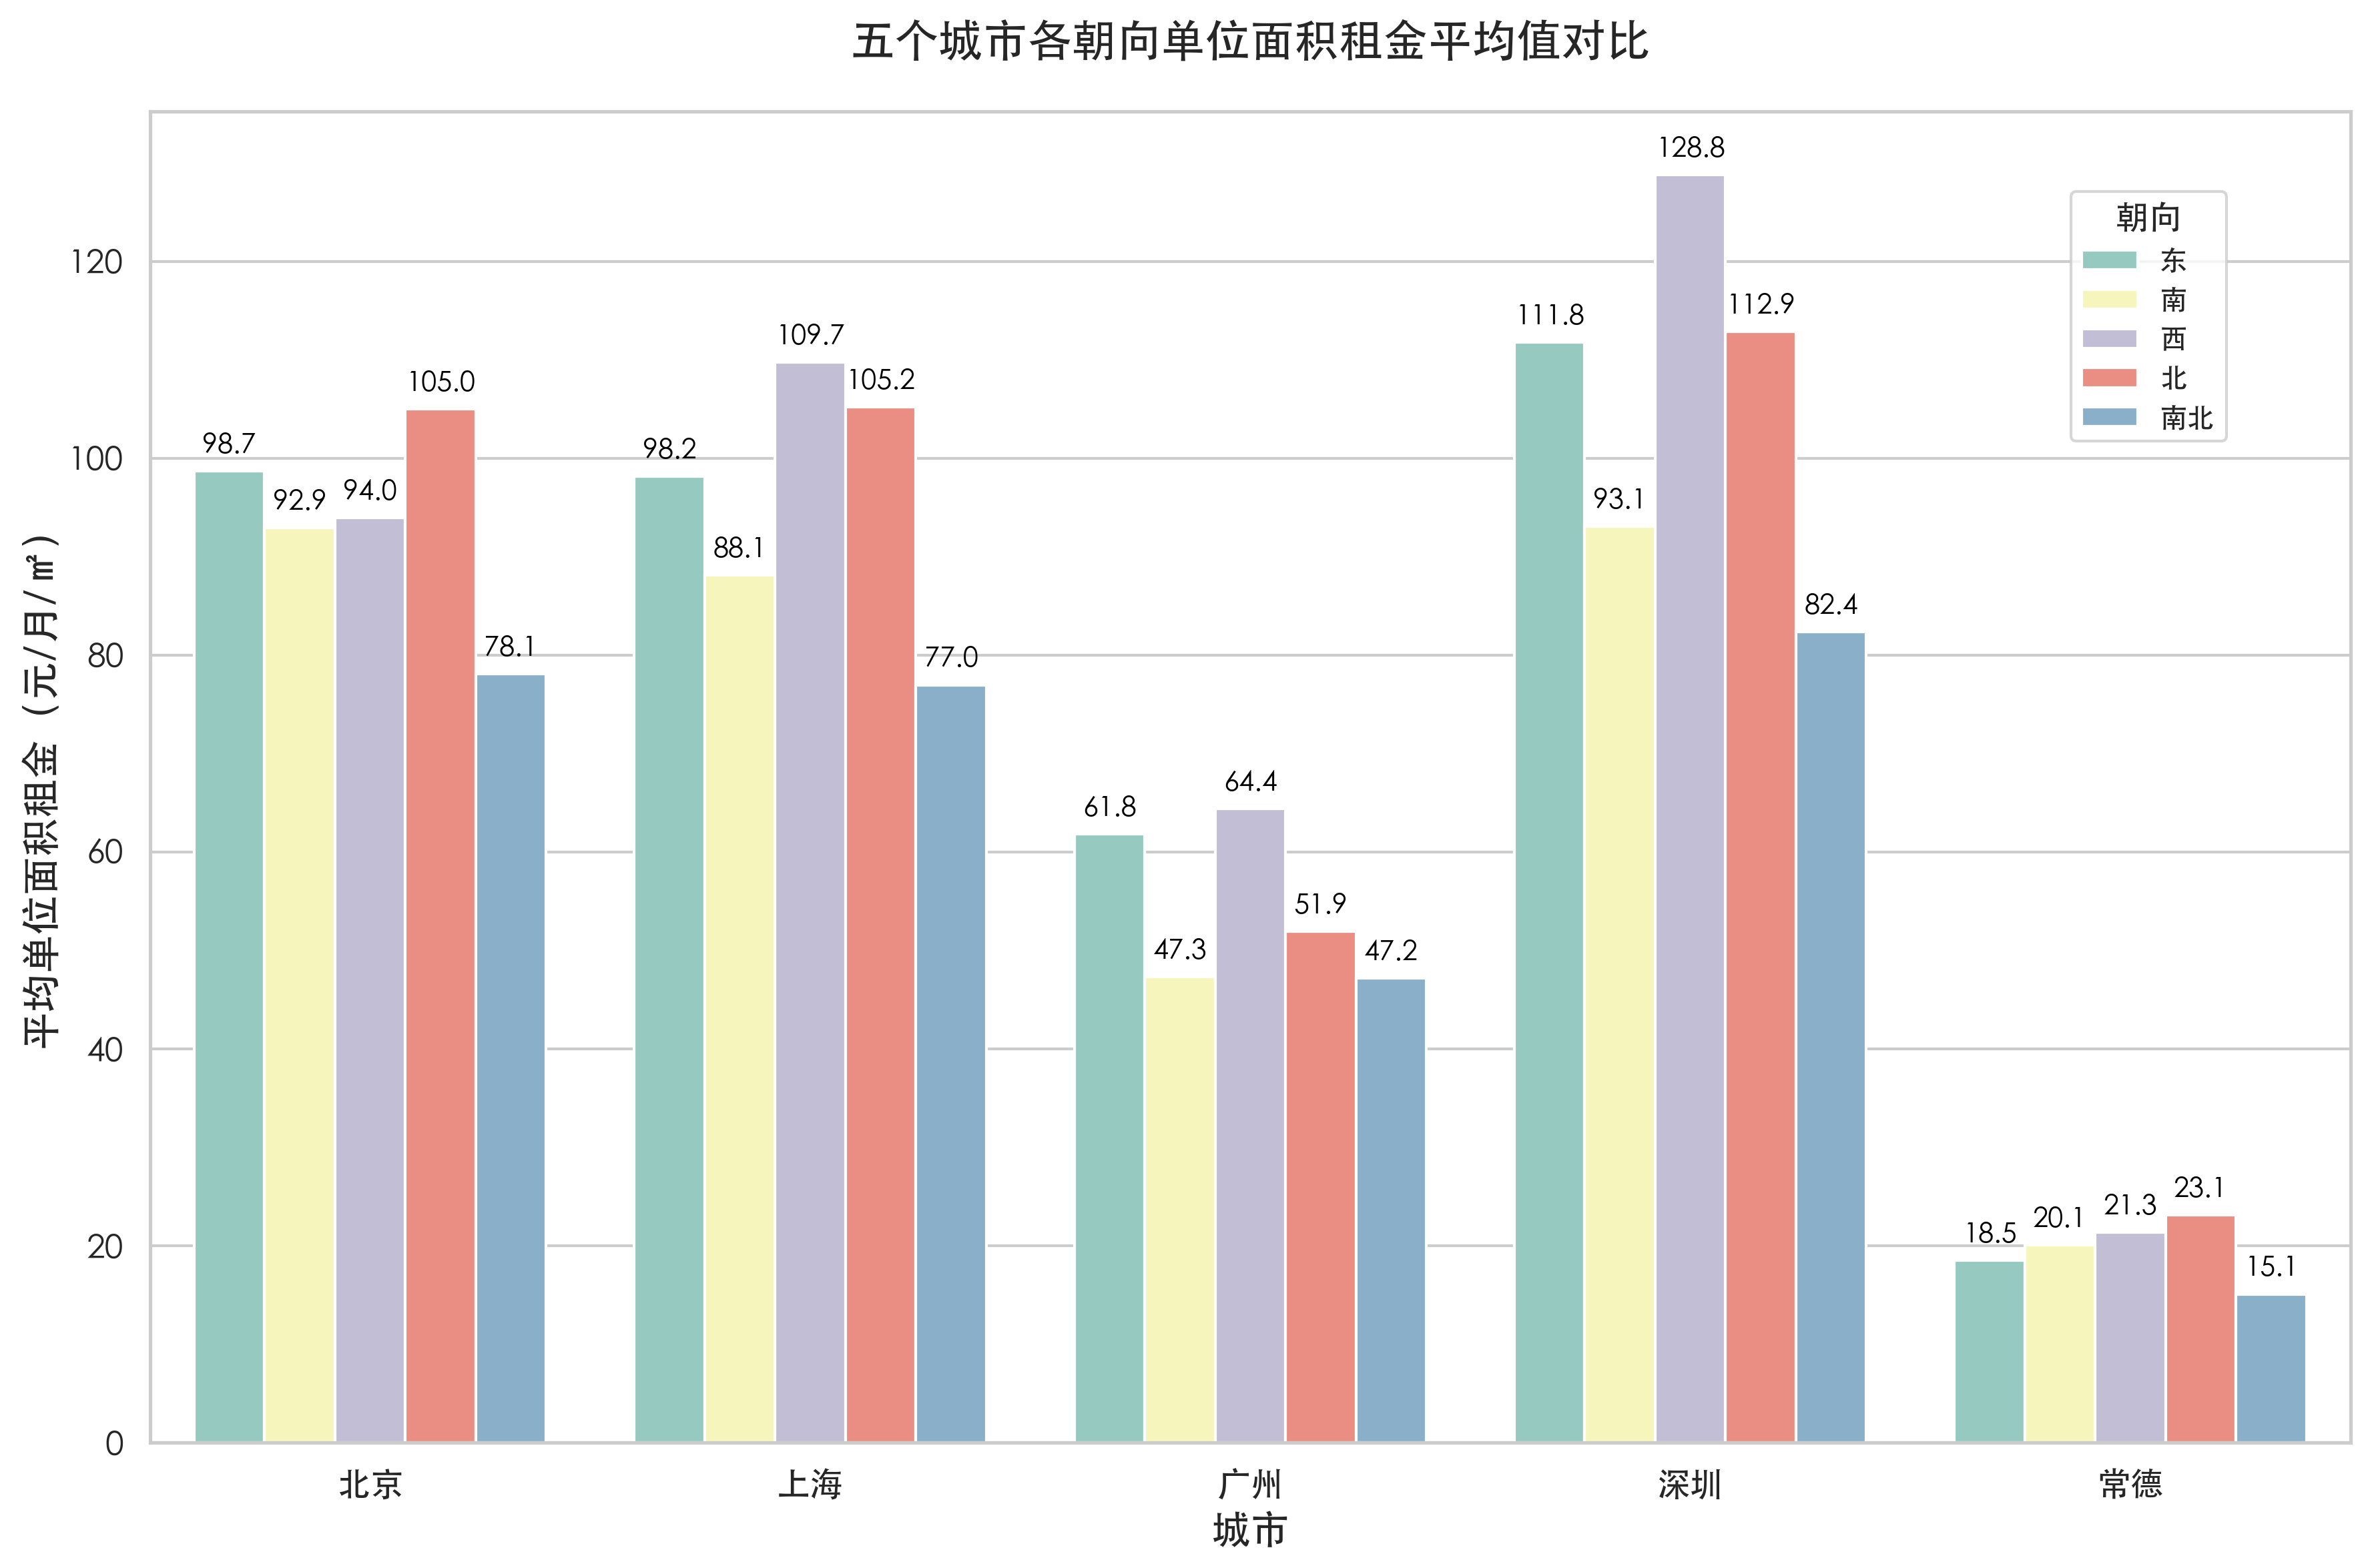
\includegraphics[width=0.7\linewidth]{../../figure/direction_unit_price_bar_chart.png}
    \caption{五个城市各朝向单位面积租金平均值对比}
    \label{fig:direction_unit_price_bar_chart}
\end{figure}

为了更精确的数值分布分析,采用箱线图进行展示,如图~\ref{fig:direction_unit_price_box_chart}。
\begin{figure}[htbp]
    \centering
    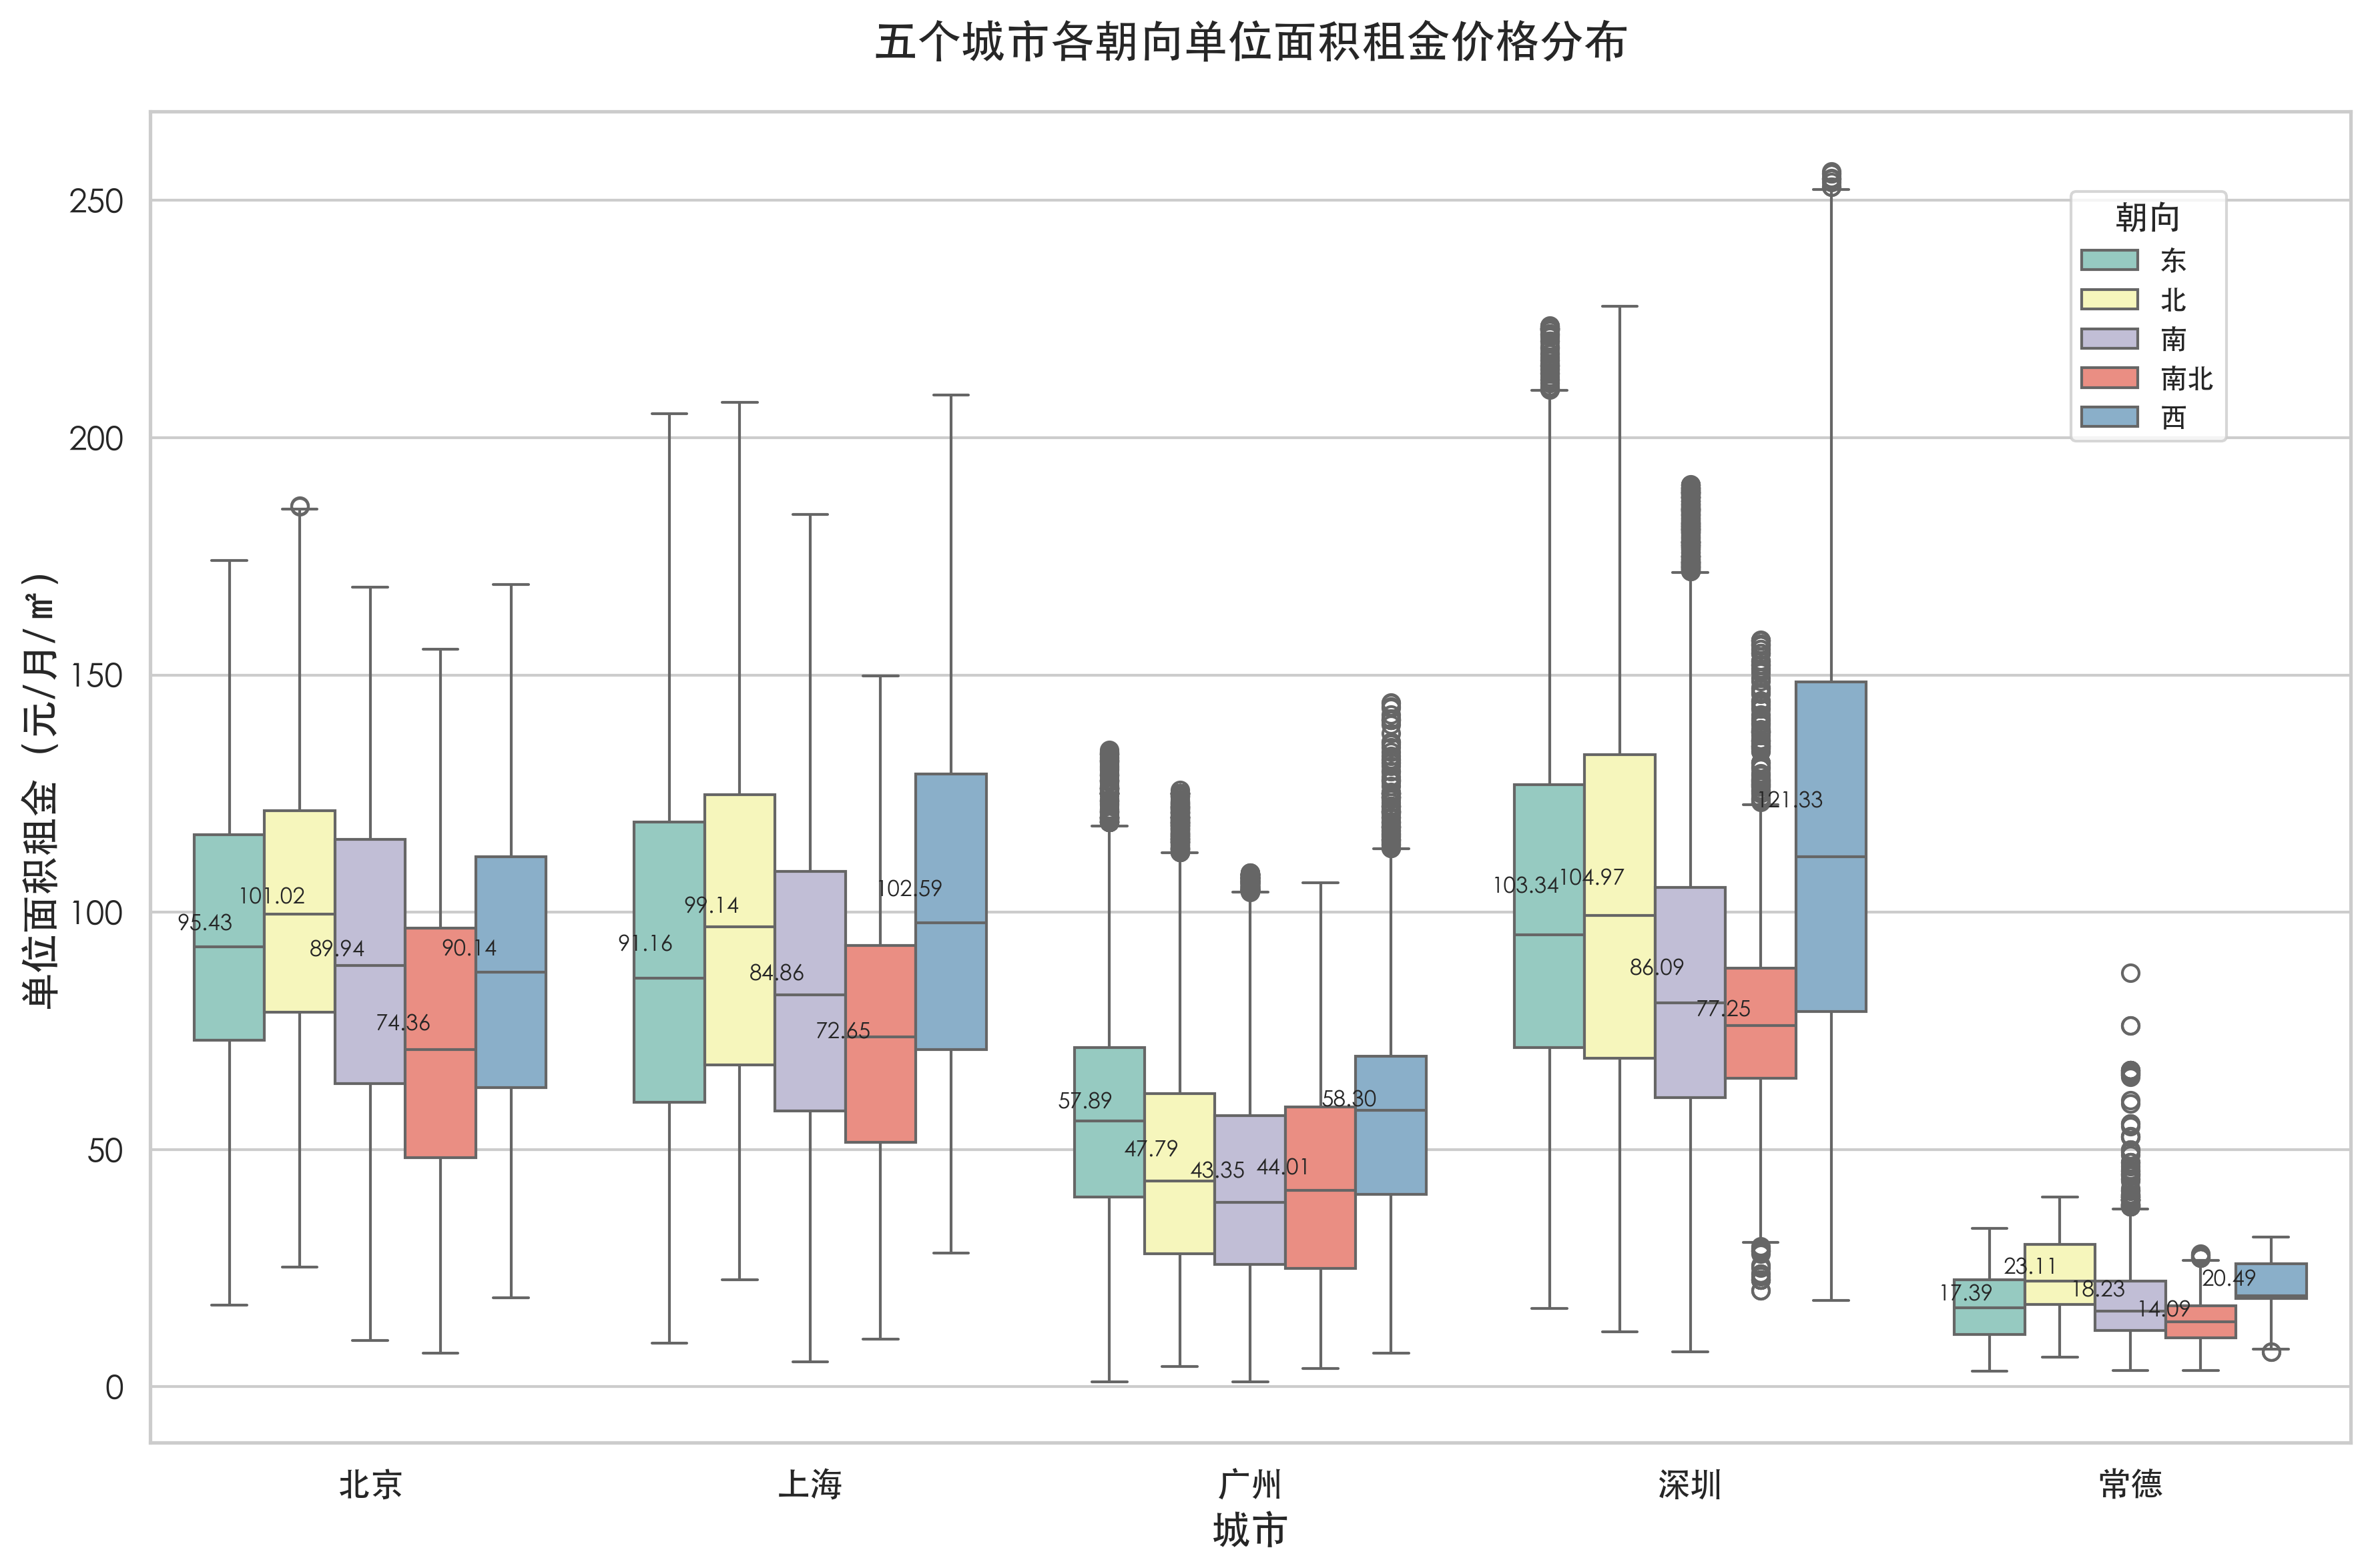
\includegraphics[width=0.7\linewidth]{../../figure/direction_unit_price_box_chart.png}
    \caption{五个城市各朝向单位面积租金分布箱线图}
    \label{fig:direction_unit_price_box_chart}
\end{figure}

从分析图可以看出,北京和常德都是向北的租房租金最高,而上海、广州、深圳都是向西的租房租金最高,传统意义的好房南北朝向的反而都是租金最低的。

原因可能在于北京和常德位于中国北方或中部,冬季寒冷,现在又是冬季,人们更注重房屋的保温性能和采光。朝北的房屋可能在设计中考虑了避风和保暖问题,而实际上的光照条件可能比预期好,因此租金较高。上海、广州和深圳位于南方,气候温暖潮湿,夏季高温潮湿,人们偏好避免阳光直射的房屋。朝西的房屋在傍晚采光较好,而避免了南方夏季正午的烈日,因此更受青睐。南北朝向的房屋可能由于通风过强(北方)或夏季过热(南方)不符合租户的需求,因此租金较低。

此外,还可能与城市规划和建筑布局,以及市场供求有关。可能存在幸存者偏差,由于南北朝向更受欢迎,这些房子已经被租走,剩下的南北朝向房屋可能是市场上的次优选择,因此租金较低。另外,还会收到数据采集和统计因素的影响,还有很多相关因素例如房高没有考虑进来,因此会存在偏差。

\subsection{人均 GDP 分析}
从\href{https://data.stats.gov.cn/index.htm}{国家统计局}网站上获取 2023 人均 GDP 数据。做出五个城市人均 GDP 直方图以及价格分布,如图~\ref{fig:gdp_bar_chart}
\begin{figure}[htbp]
    \centering
    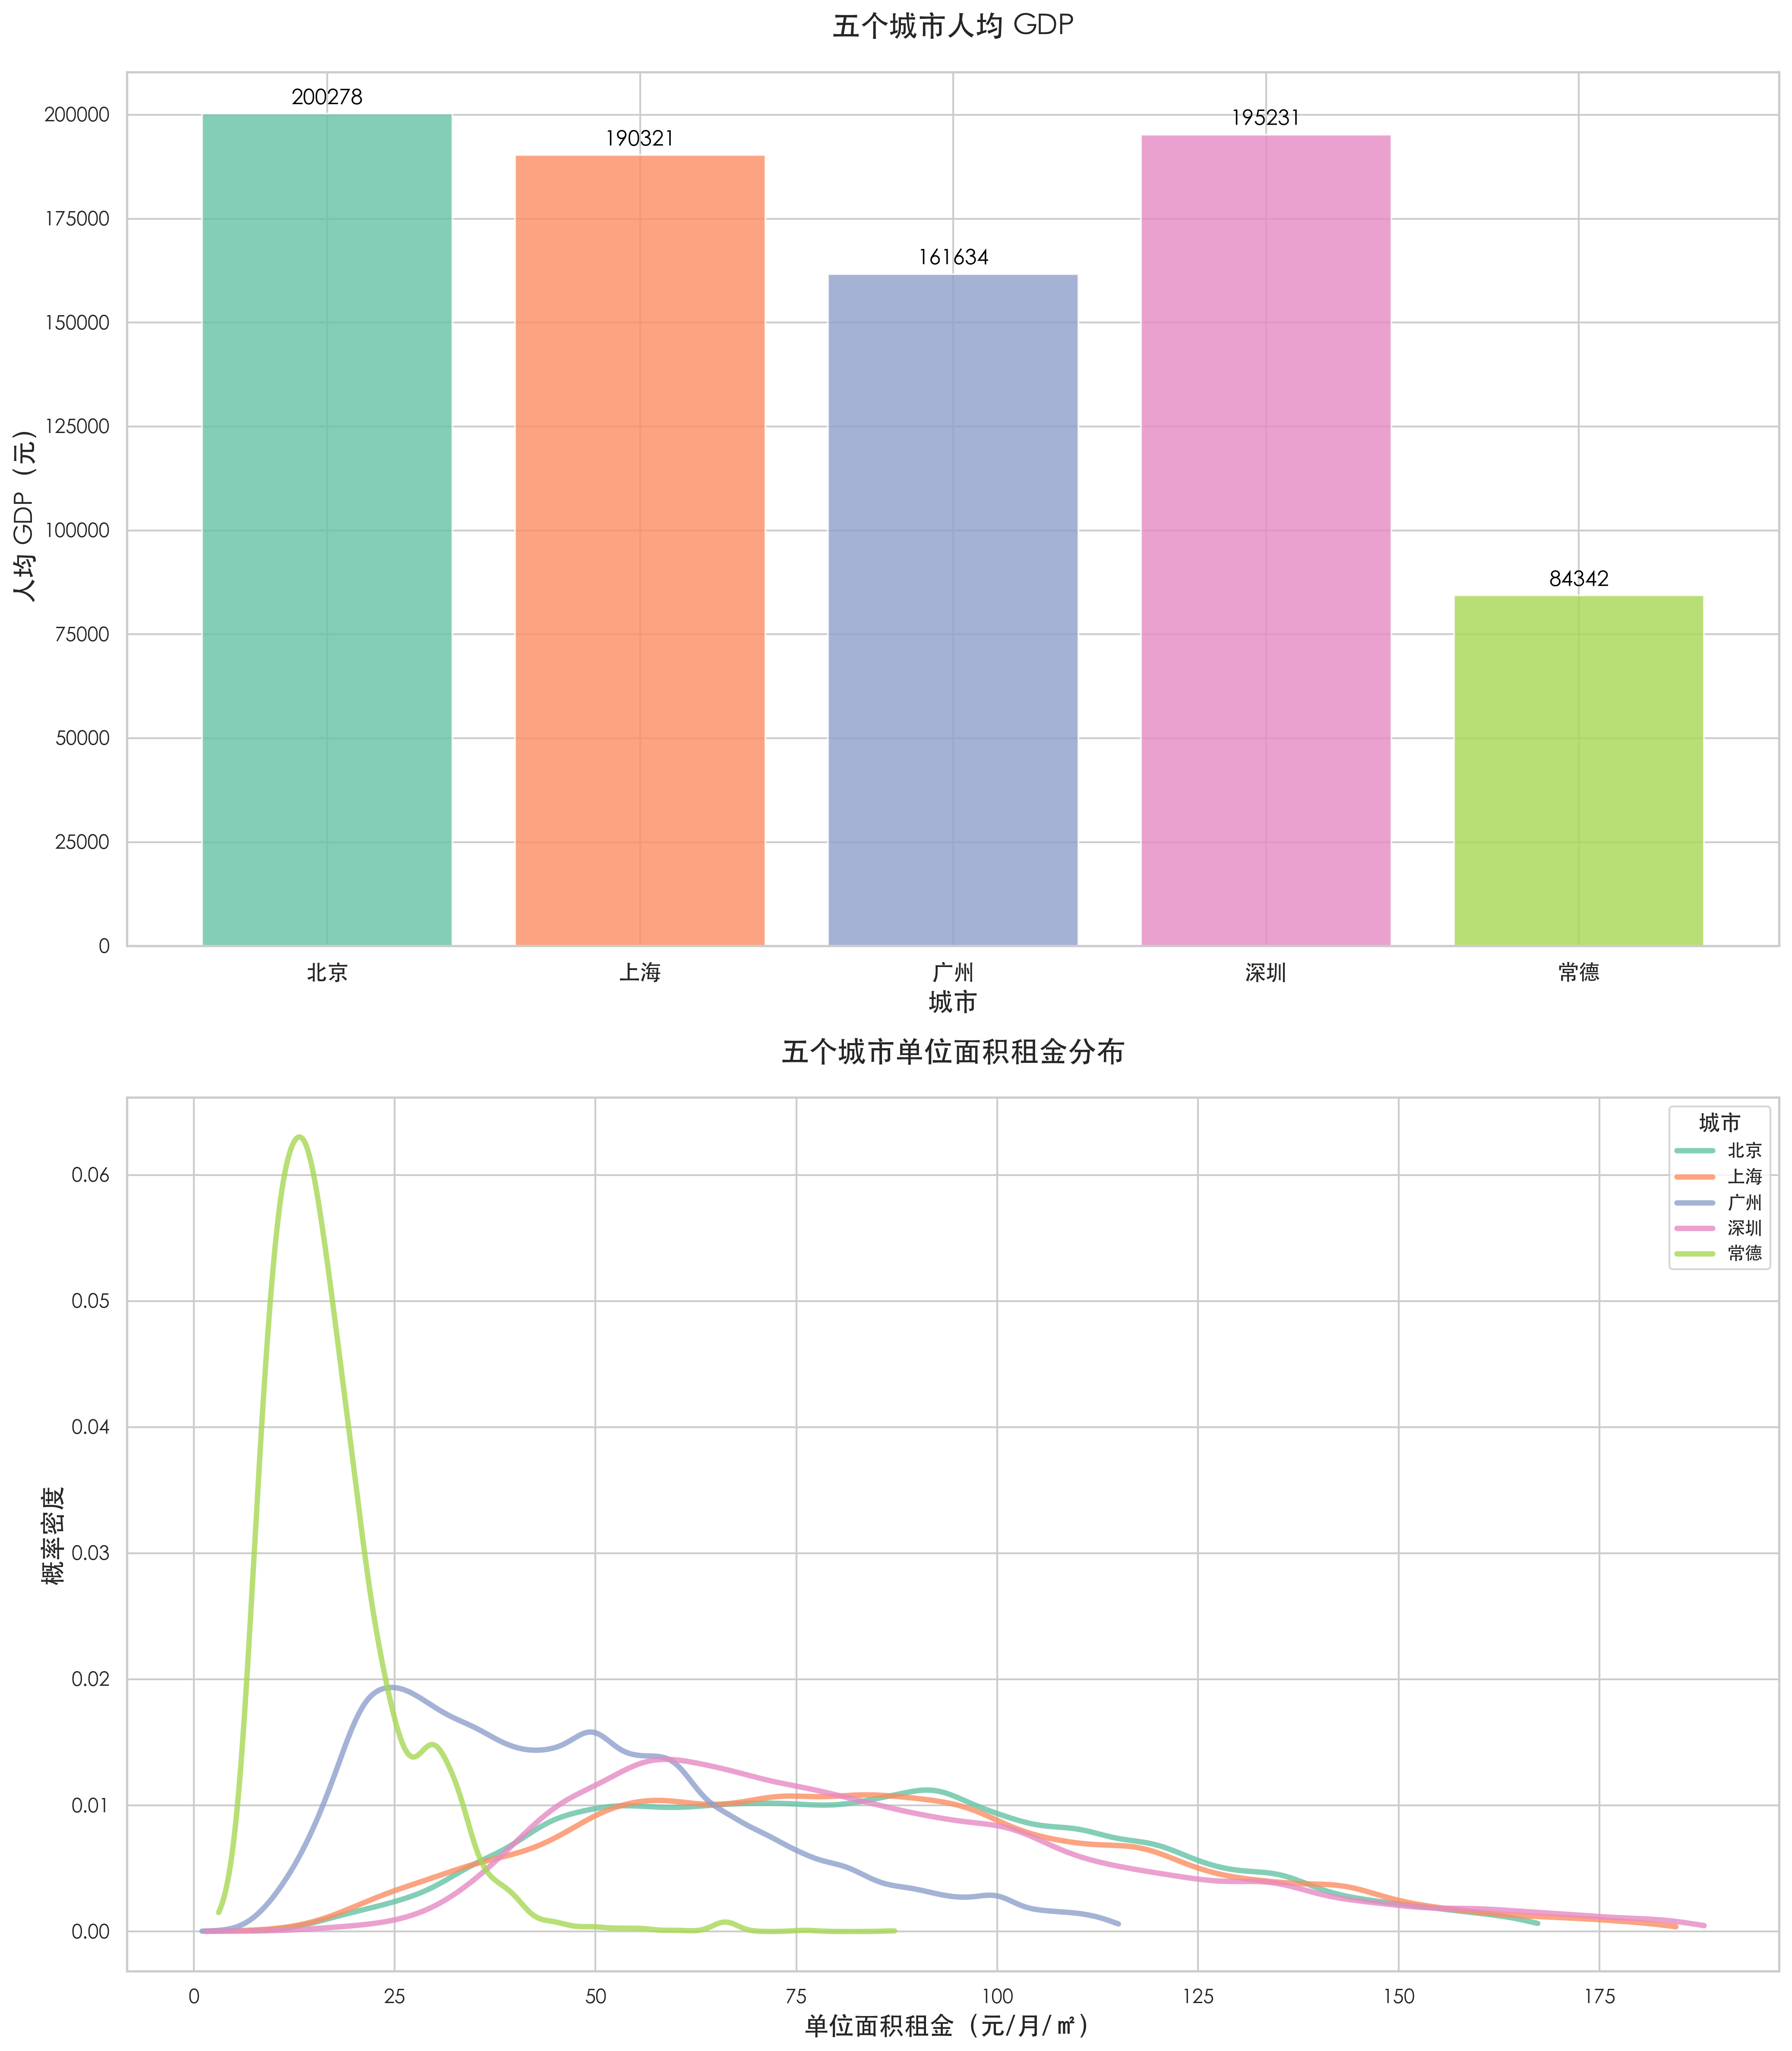
\includegraphics[width=0.7\linewidth]{../../figure/gdp_unit_price_chart.png}
    \caption{五个城市人均GDP以及单位面积租金分布}
    \label{fig:gdp_bar_chart}
\end{figure}

为了比较性价比,我们定义租房性价比指数(CPI)为\[
    \text{CPI} = \frac{\text{人均GDP}}{\text{单位面积租金}}
\]
CPI 越高代表性价比越高。如图~\ref{fig:gdp_unit_price_scatter_chart}、图~\ref{fig:cpi_bar_chart}、图~\ref{fig:gdp_price_scatter_chart}。
\begin{figure}[htbp]
    \centering
    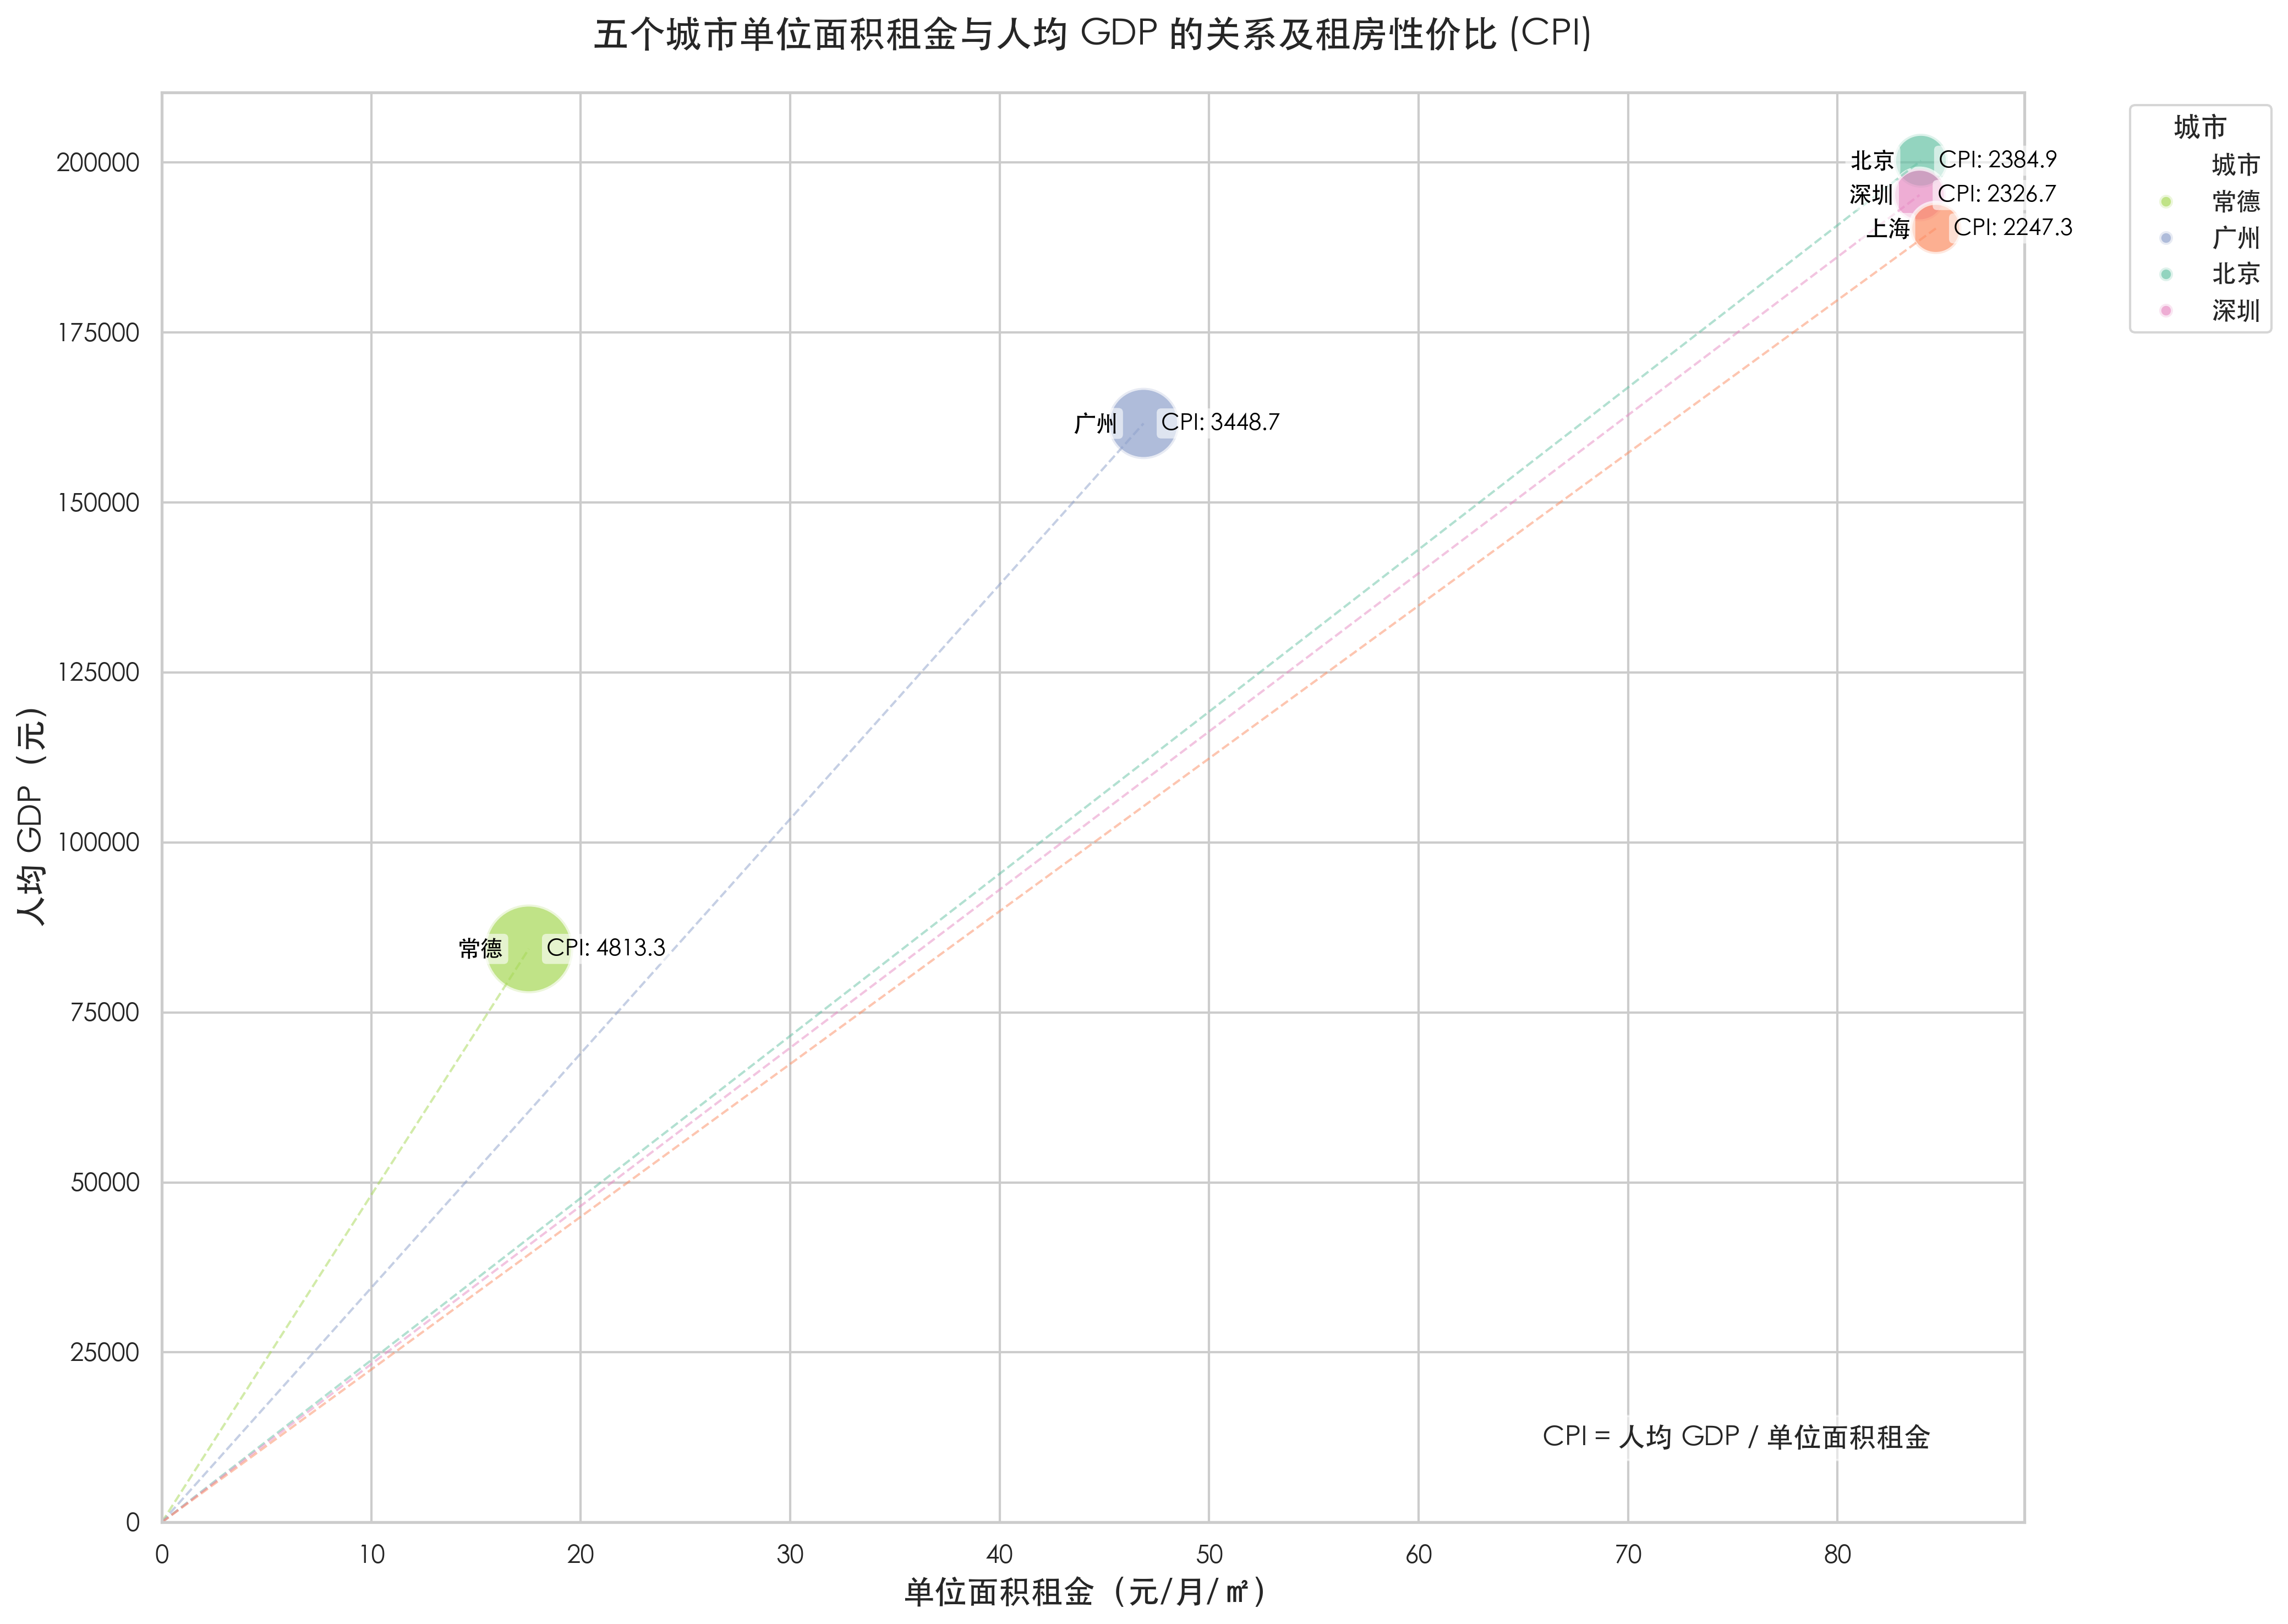
\includegraphics[width=0.7\linewidth]{../../figure/gdp_unit_price_scatter_chart.png}
    \caption{五个城市单位面积租金与人均GDP的关系及租房性价比(CPI)}
    \label{fig:gdp_unit_price_scatter_chart}
\end{figure}
\begin{figure}[htbp]
    \centering
    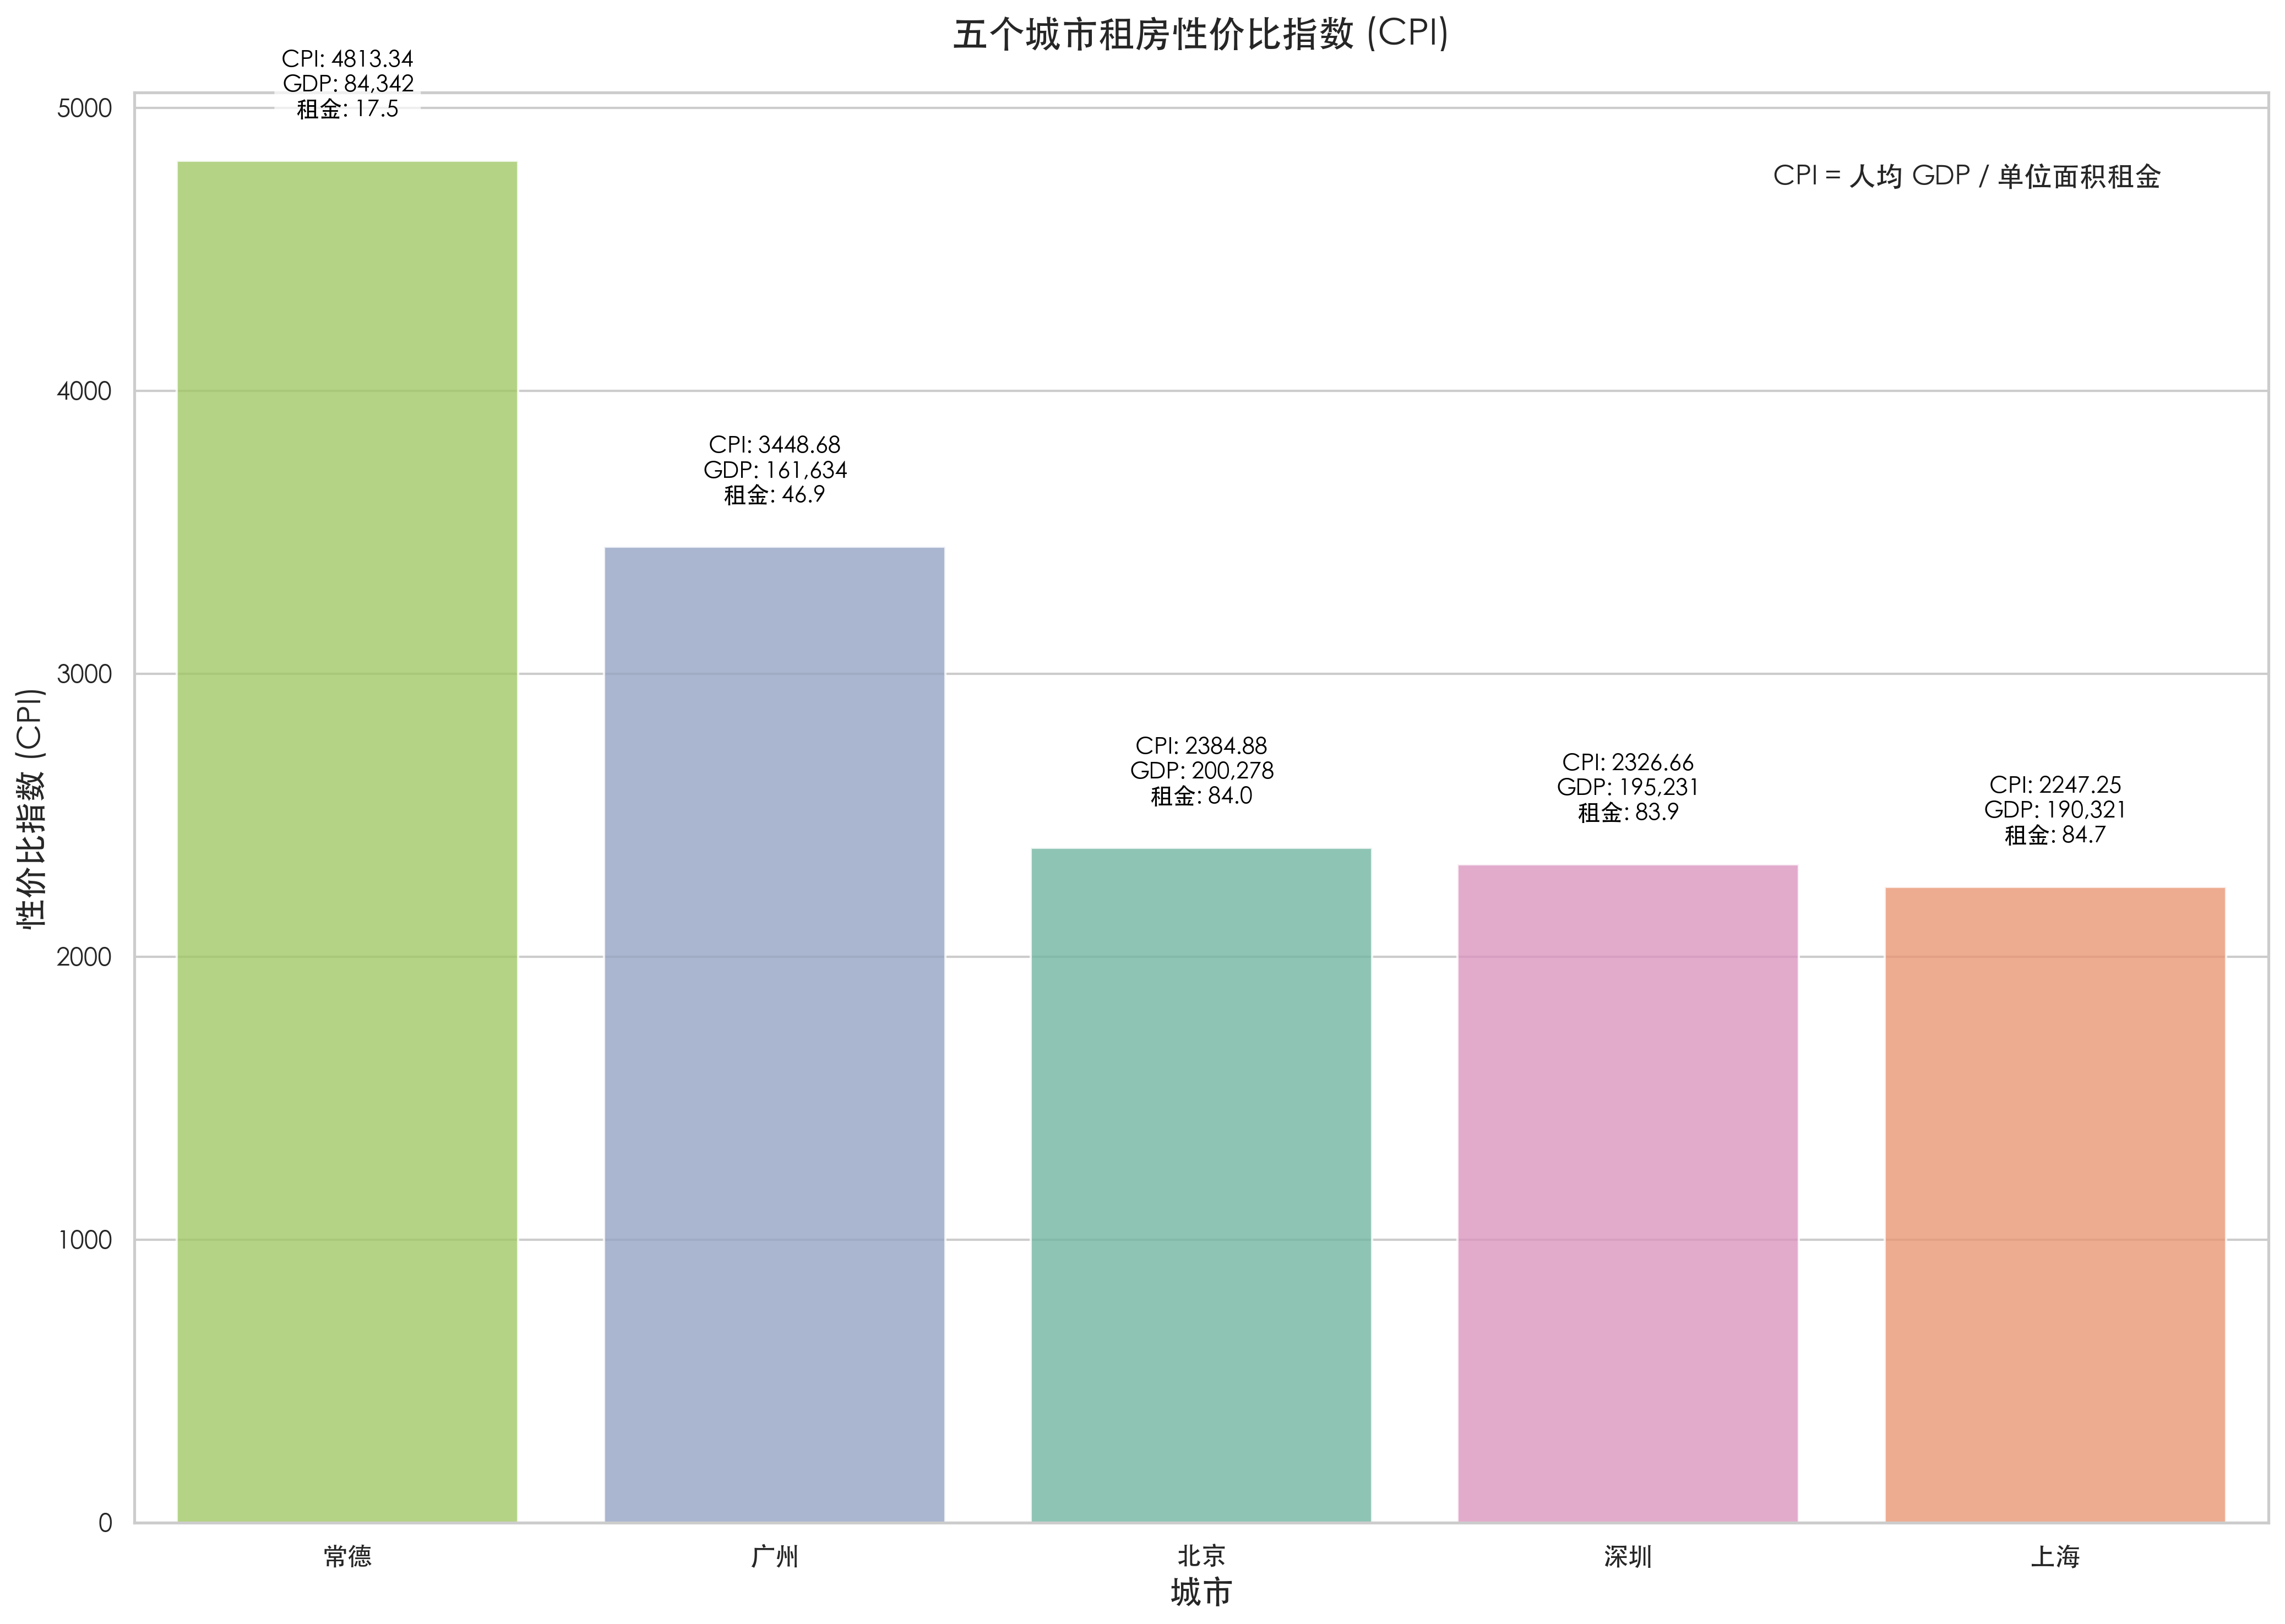
\includegraphics[width=0.7\linewidth]{../../figure/cpi_bar_chart.png}
    \caption{五个城市租房性价比指数(CPI)}
    \label{fig:cpi_bar_chart}
\end{figure}

同时对总价而非单位面积租金进行分析,如图~\ref{fig:gdp_price_scatter_chart}。
\begin{figure}[htbp]
    \centering
    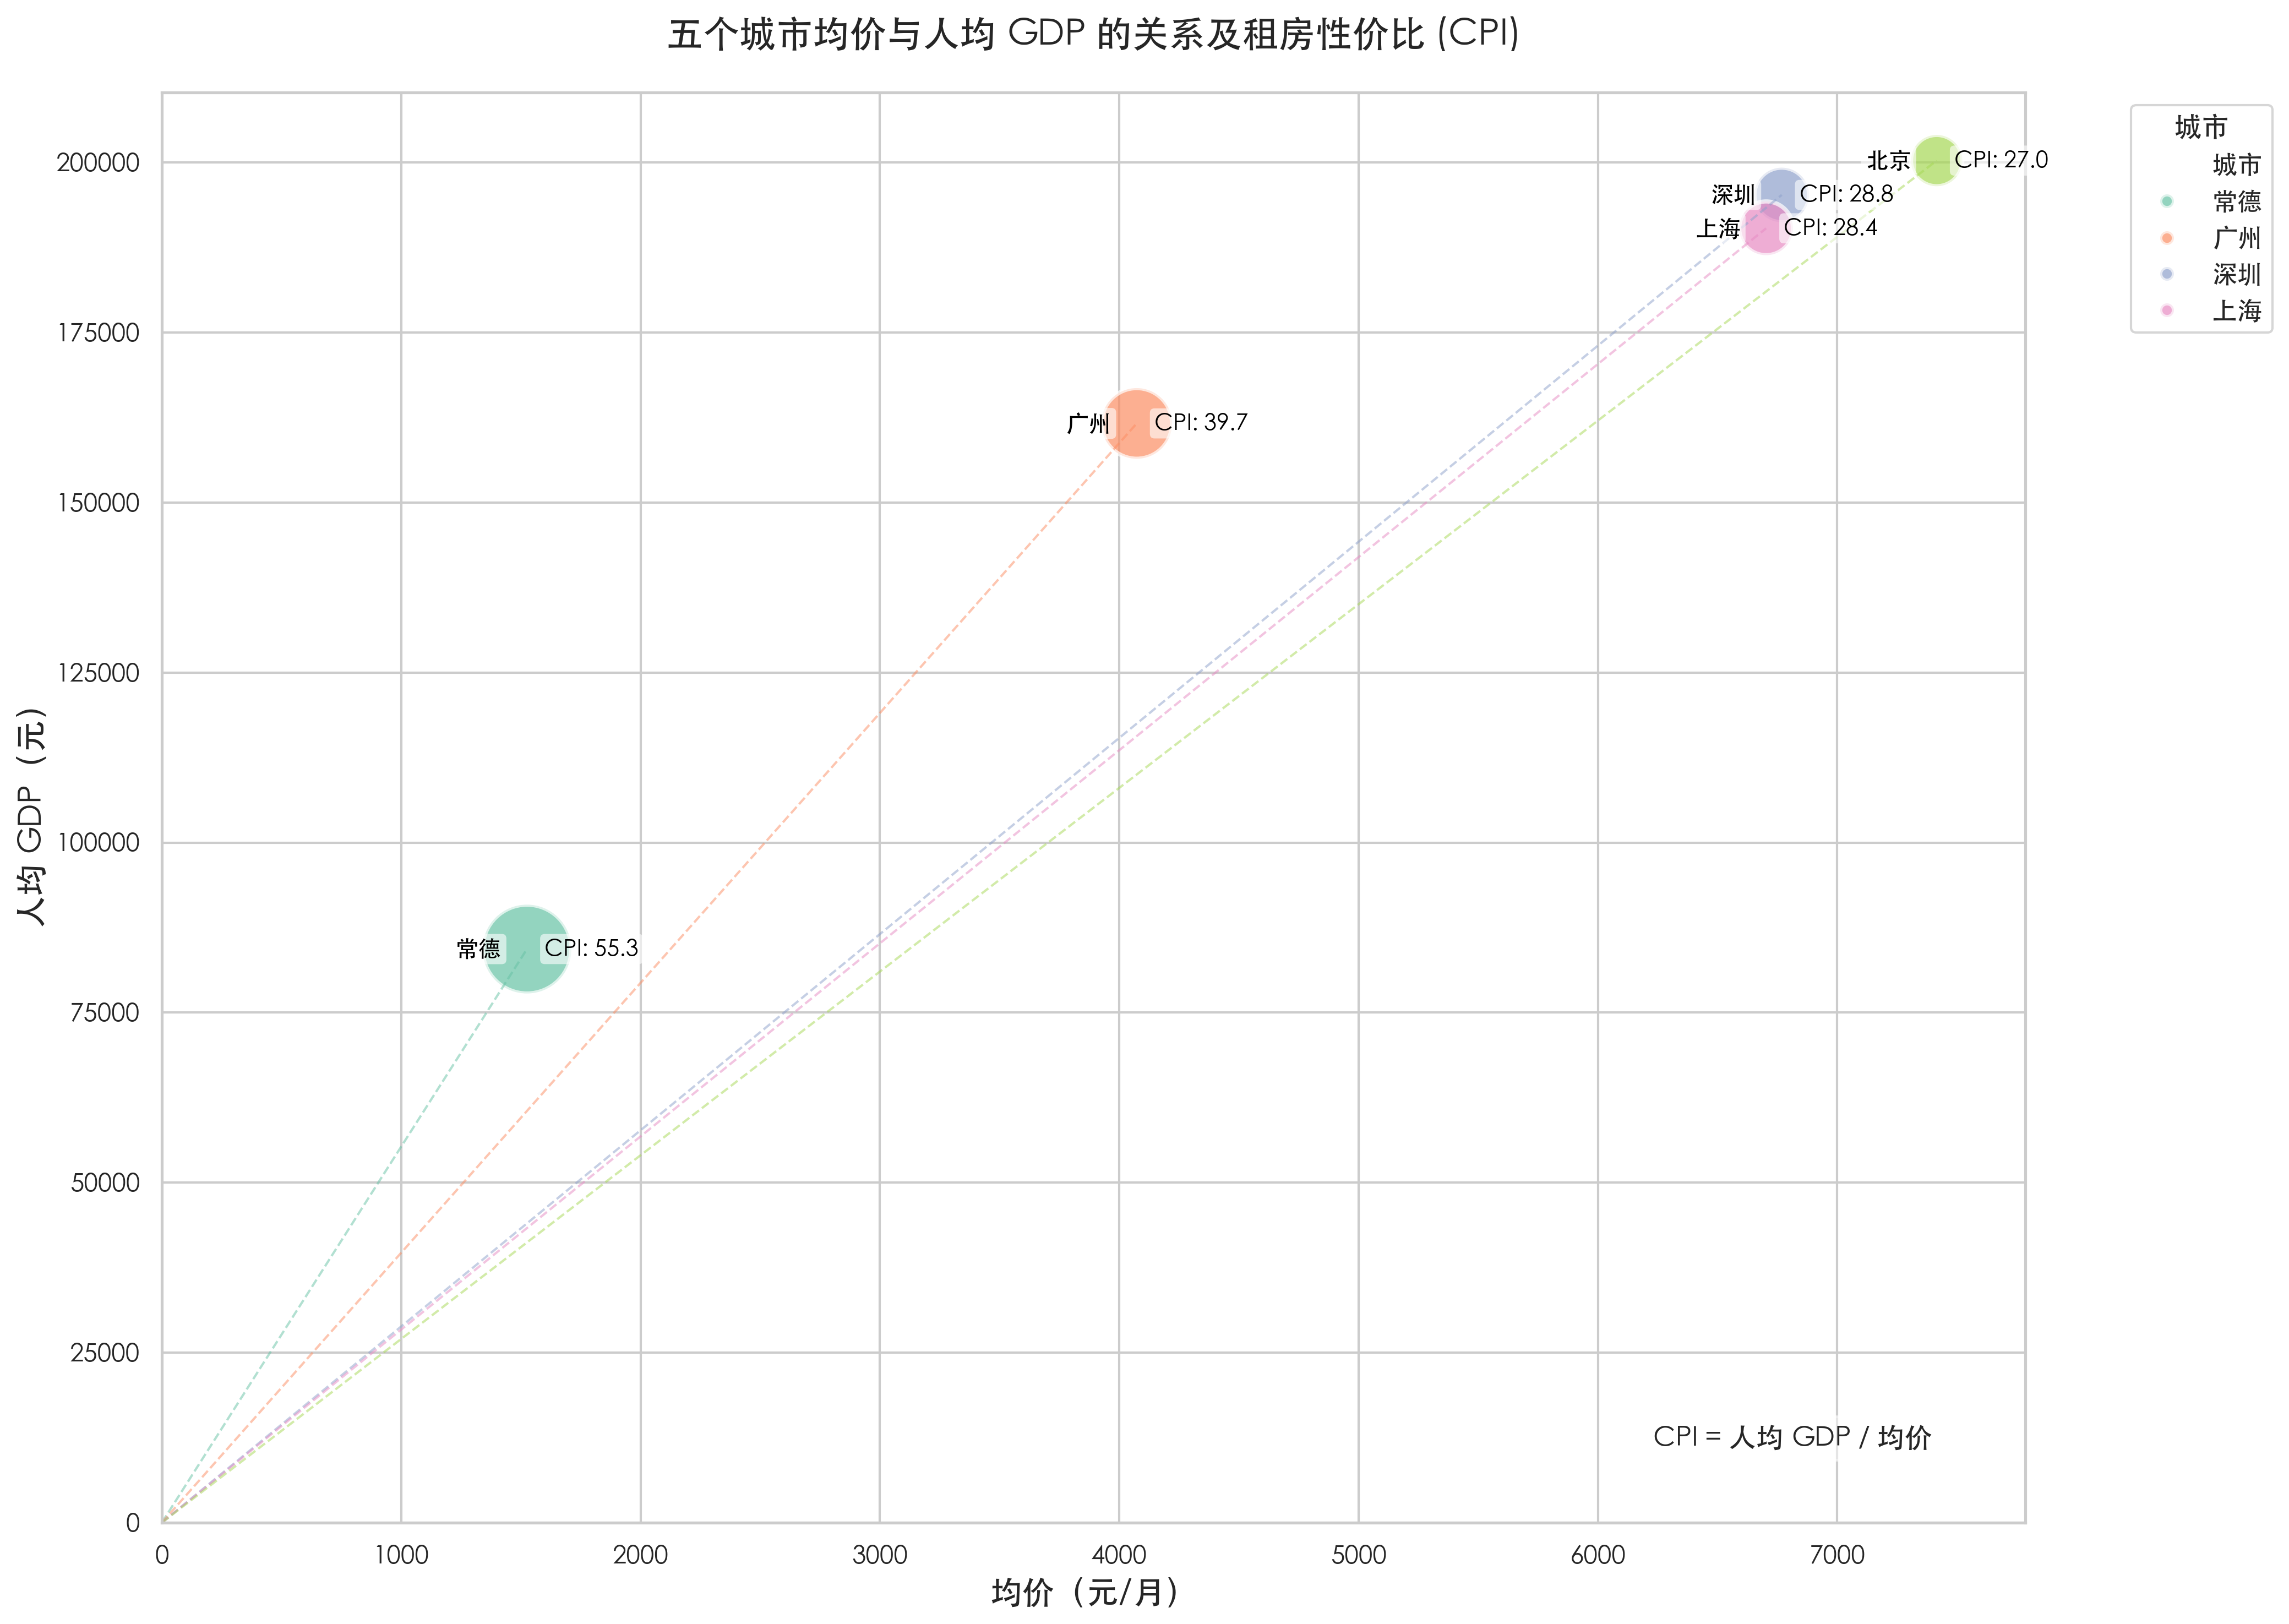
\includegraphics[width=0.7\linewidth]{../../figure/gdp_price_scatter_chart.png}
    \caption{五个城市均价与人均GDP的关系及租房性价比(CPI)}
    \label{fig:gdp_price_scatter_chart}
\end{figure}
在散点图中,越靠近左上,代表单位面积租金低的同时,人均 GDP 高,性价比越高。由 CPI 的定义,可以知道,斜率即 CPI。可以看出,北京、上海、广州、深圳等一线大城市的性价比较低,而常德的性价比较高,虽然其 GDP 较低,但是租金明显较低,因此性价比较高。

在四大城市中,从单价看,性价比排名为广州、北京、深圳、上海。从总价看,为广州、深圳、上海、北京。可以看出,广州在大城市中性价比较高。

\subsection{平均工资分析}
分析与人均 GDP 类似,从各政府统计局网站(\href{https://si12333.cn/policy/mfray.html}{北京上海}、\href{https://gz12345.gz.gov.cn/kmInterf/kmPointDetail.do?id=1400739&searchName=平均工资&0.053973112663851186}{广州}、\href{https://www.sz.gov.cn/cn/xxgk/zfxxgj/tjsj/tjgb/content/post_11398823.html}{深圳}、\href{https://tjj.changde.gov.cn/zhdt/sjdt/content_1069834}{常德})上获取 2023 平均工资数据。由于常德市仅公开了城镇非私营单位就业人员年平均工资,为了统一,所有城市均采用该标准处以 12 作为平均工资。如图~\ref{fig:salary_unit_price_chart}、图~\ref{fig:salary_unit_price_scatter_chart}、图~\ref{fig:salary_cpi_bar_chart}。
\begin{figure}[htbp]
    \centering
    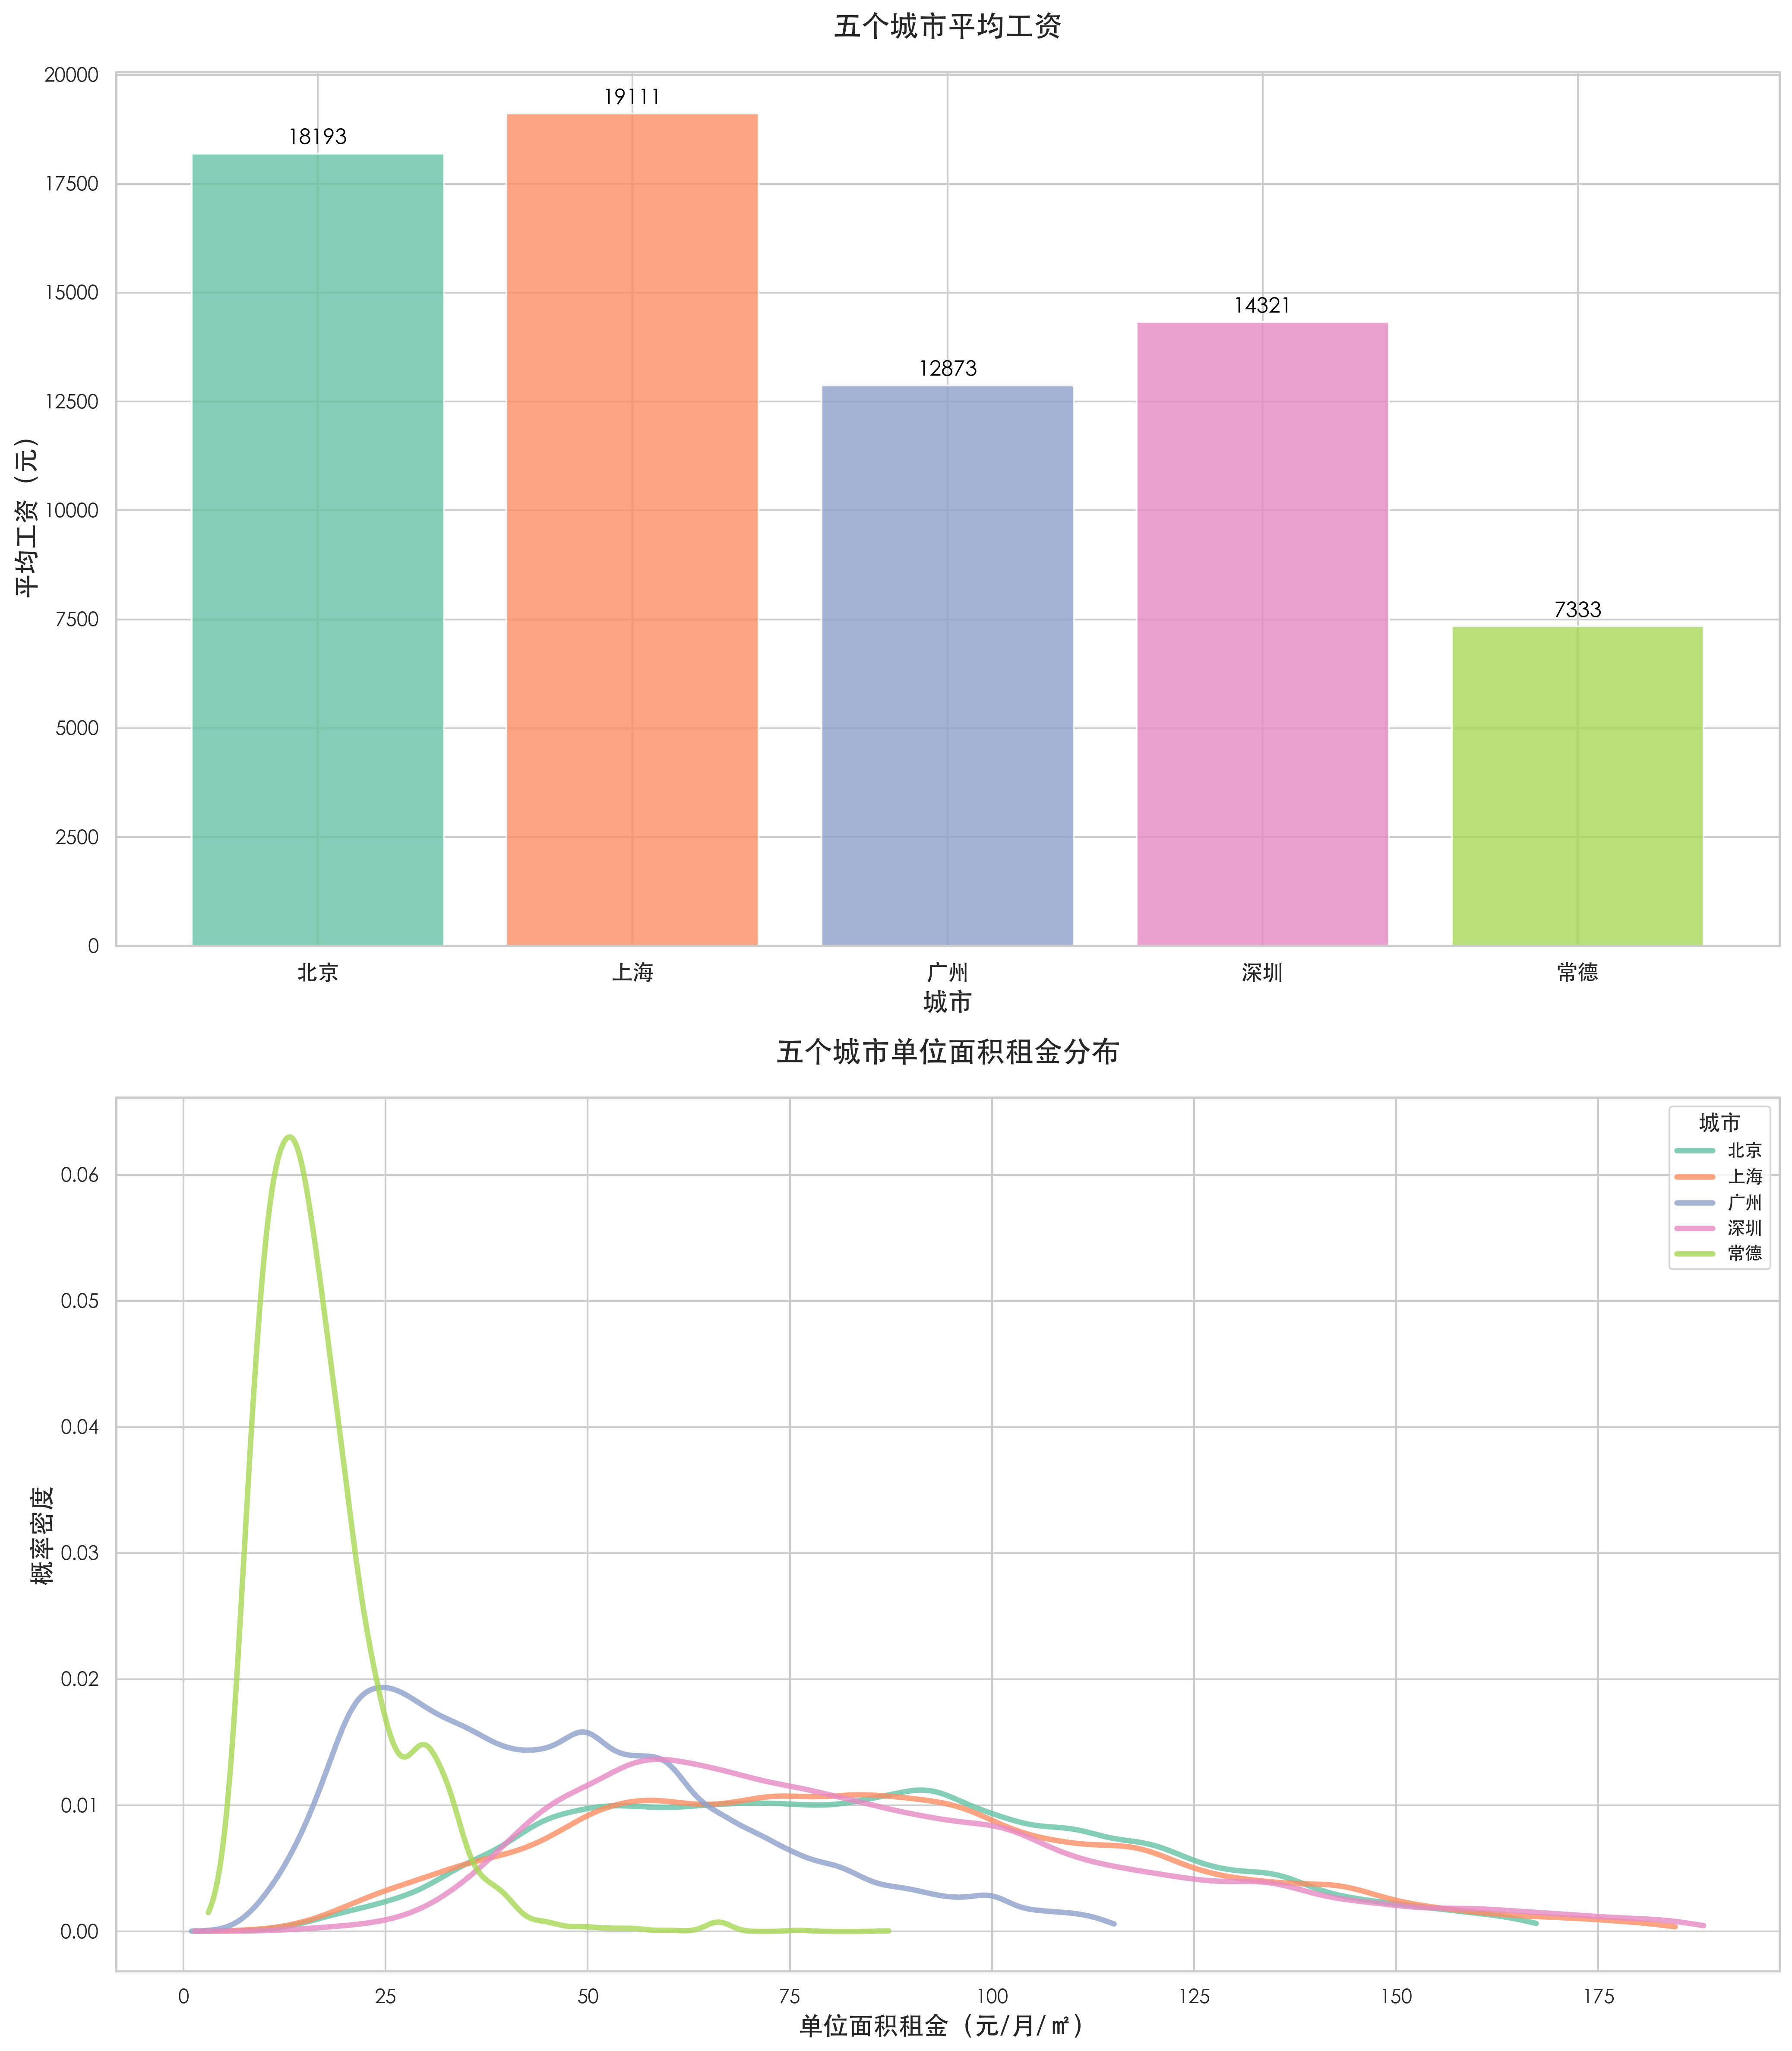
\includegraphics[width=0.7\linewidth]{../../figure/salary_unit_price_chart.png}
    \caption{五个城市平均工资以及单位面积租金分布}
    \label{fig:salary_unit_price_chart}
\end{figure}
\begin{figure}[htbp]
    \centering
    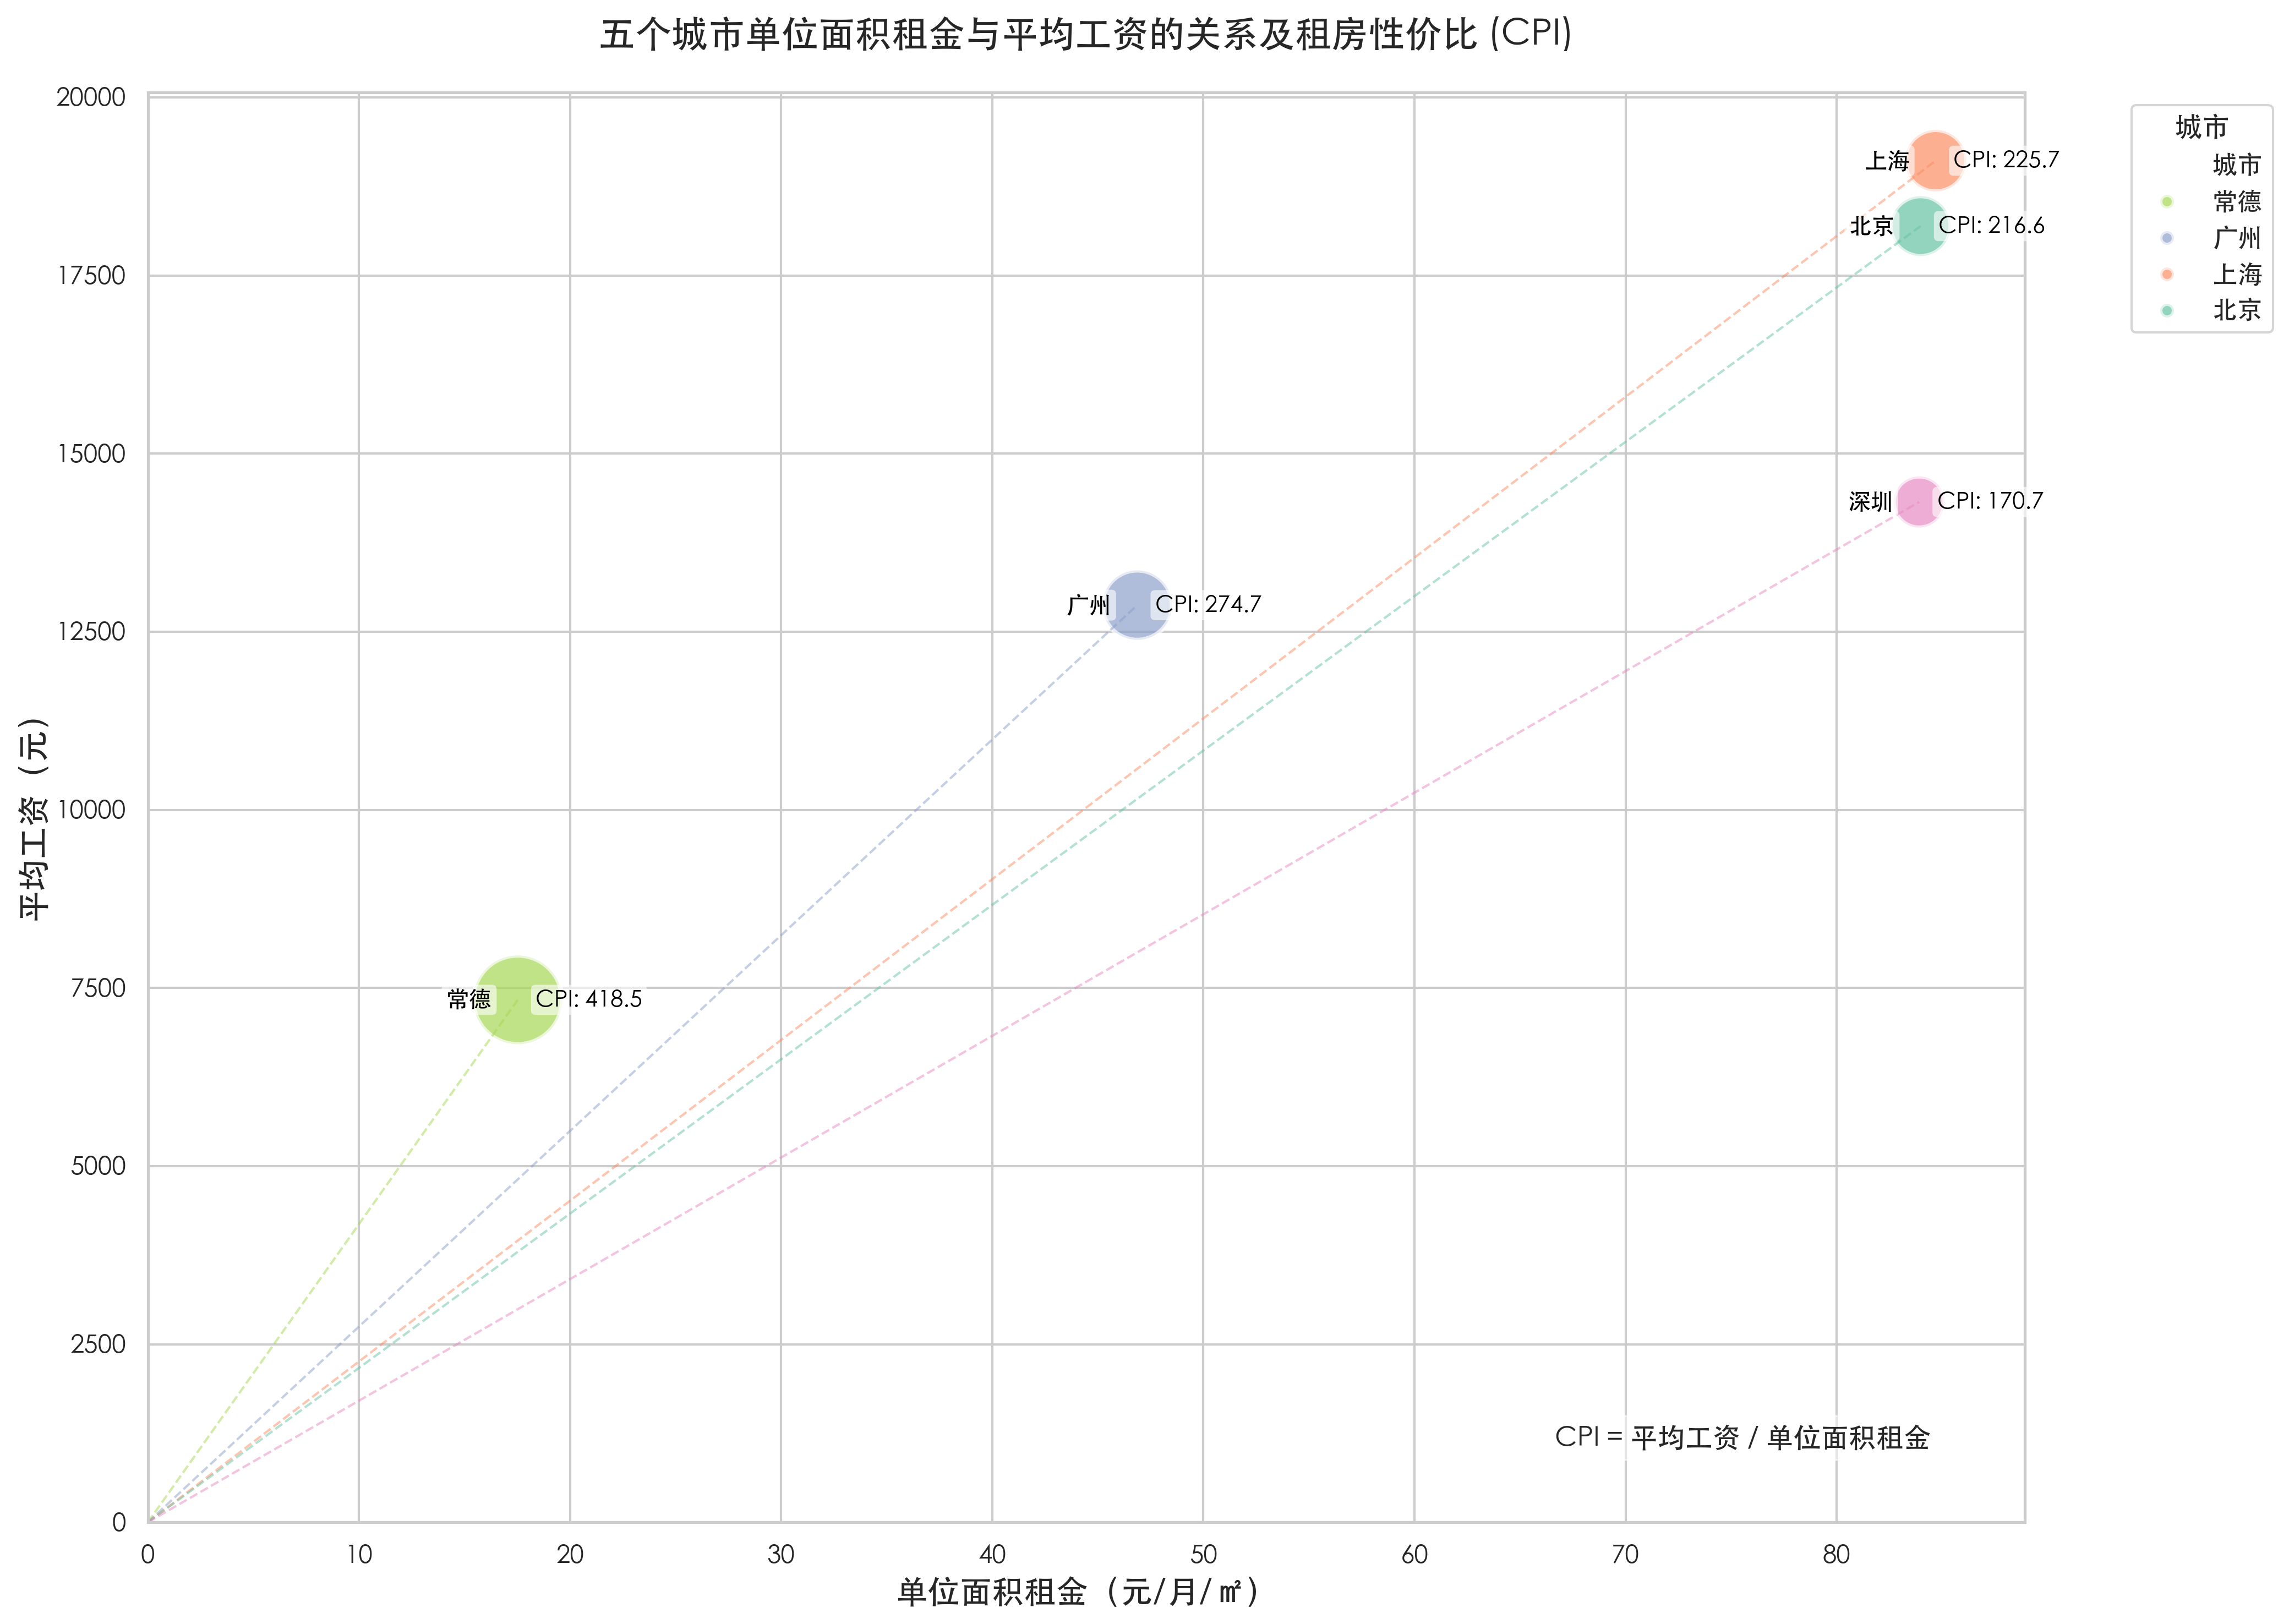
\includegraphics[width=0.7\linewidth]{../../figure/salary_unit_price_scatter_chart.png}
    \caption{五个城市单位面积租金与平均工资的关系及租房性价比(CPI)}
    \label{fig:salary_unit_price_scatter_chart}
\end{figure}
\begin{figure}[htbp]
    \centering
    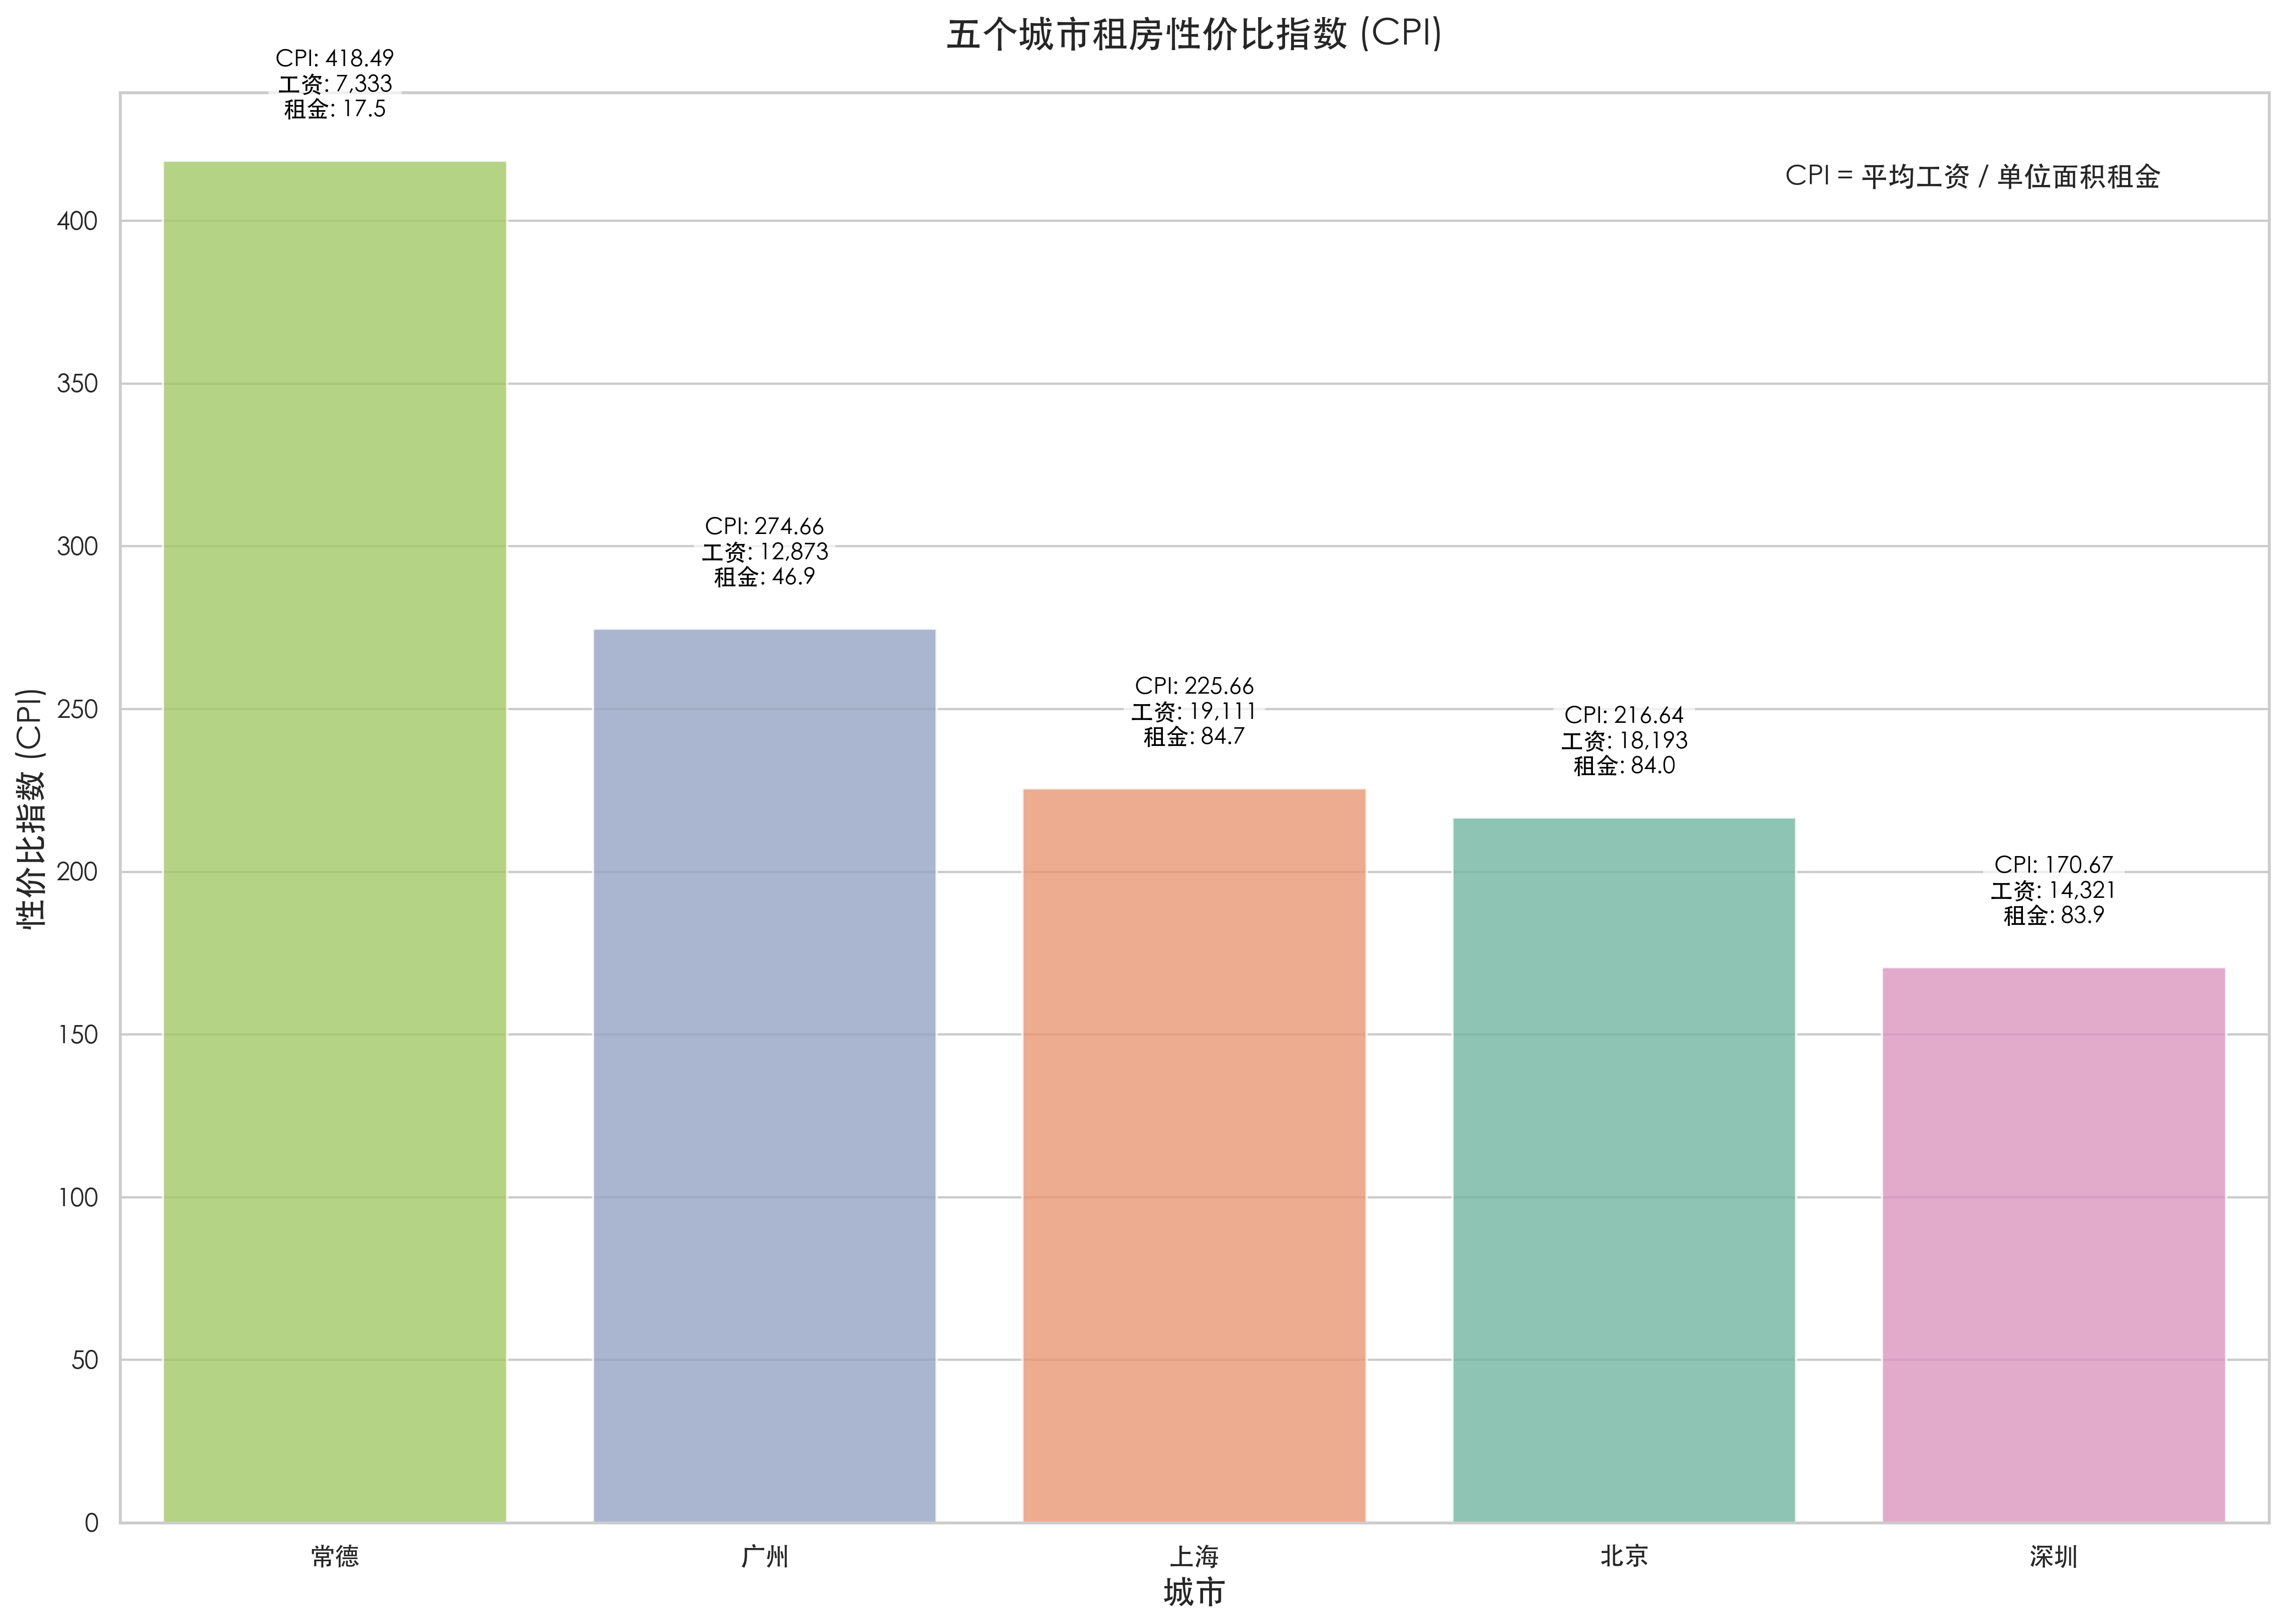
\includegraphics[width=0.7\linewidth]{../../figure/salary_cpi_bar_chart.png}
    \caption{五个城市租房性价比指数(CPI)}
    \label{fig:salary_cpi_bar_chart}
\end{figure}
结论与 GDP 分析相似,常德的性价比明显较高,而北京、上海、广州、深圳等一线大城市的性价比较低。排序为广州、上海、北京、深圳。广州仍然是大城市中性价比最高的城市。

我们还对租房总价对月薪资的占比进行了分析,画出了饼图如图~\ref{fig:salary_price_pie_chart}。
\begin{figure}[htbp]
    \centering
    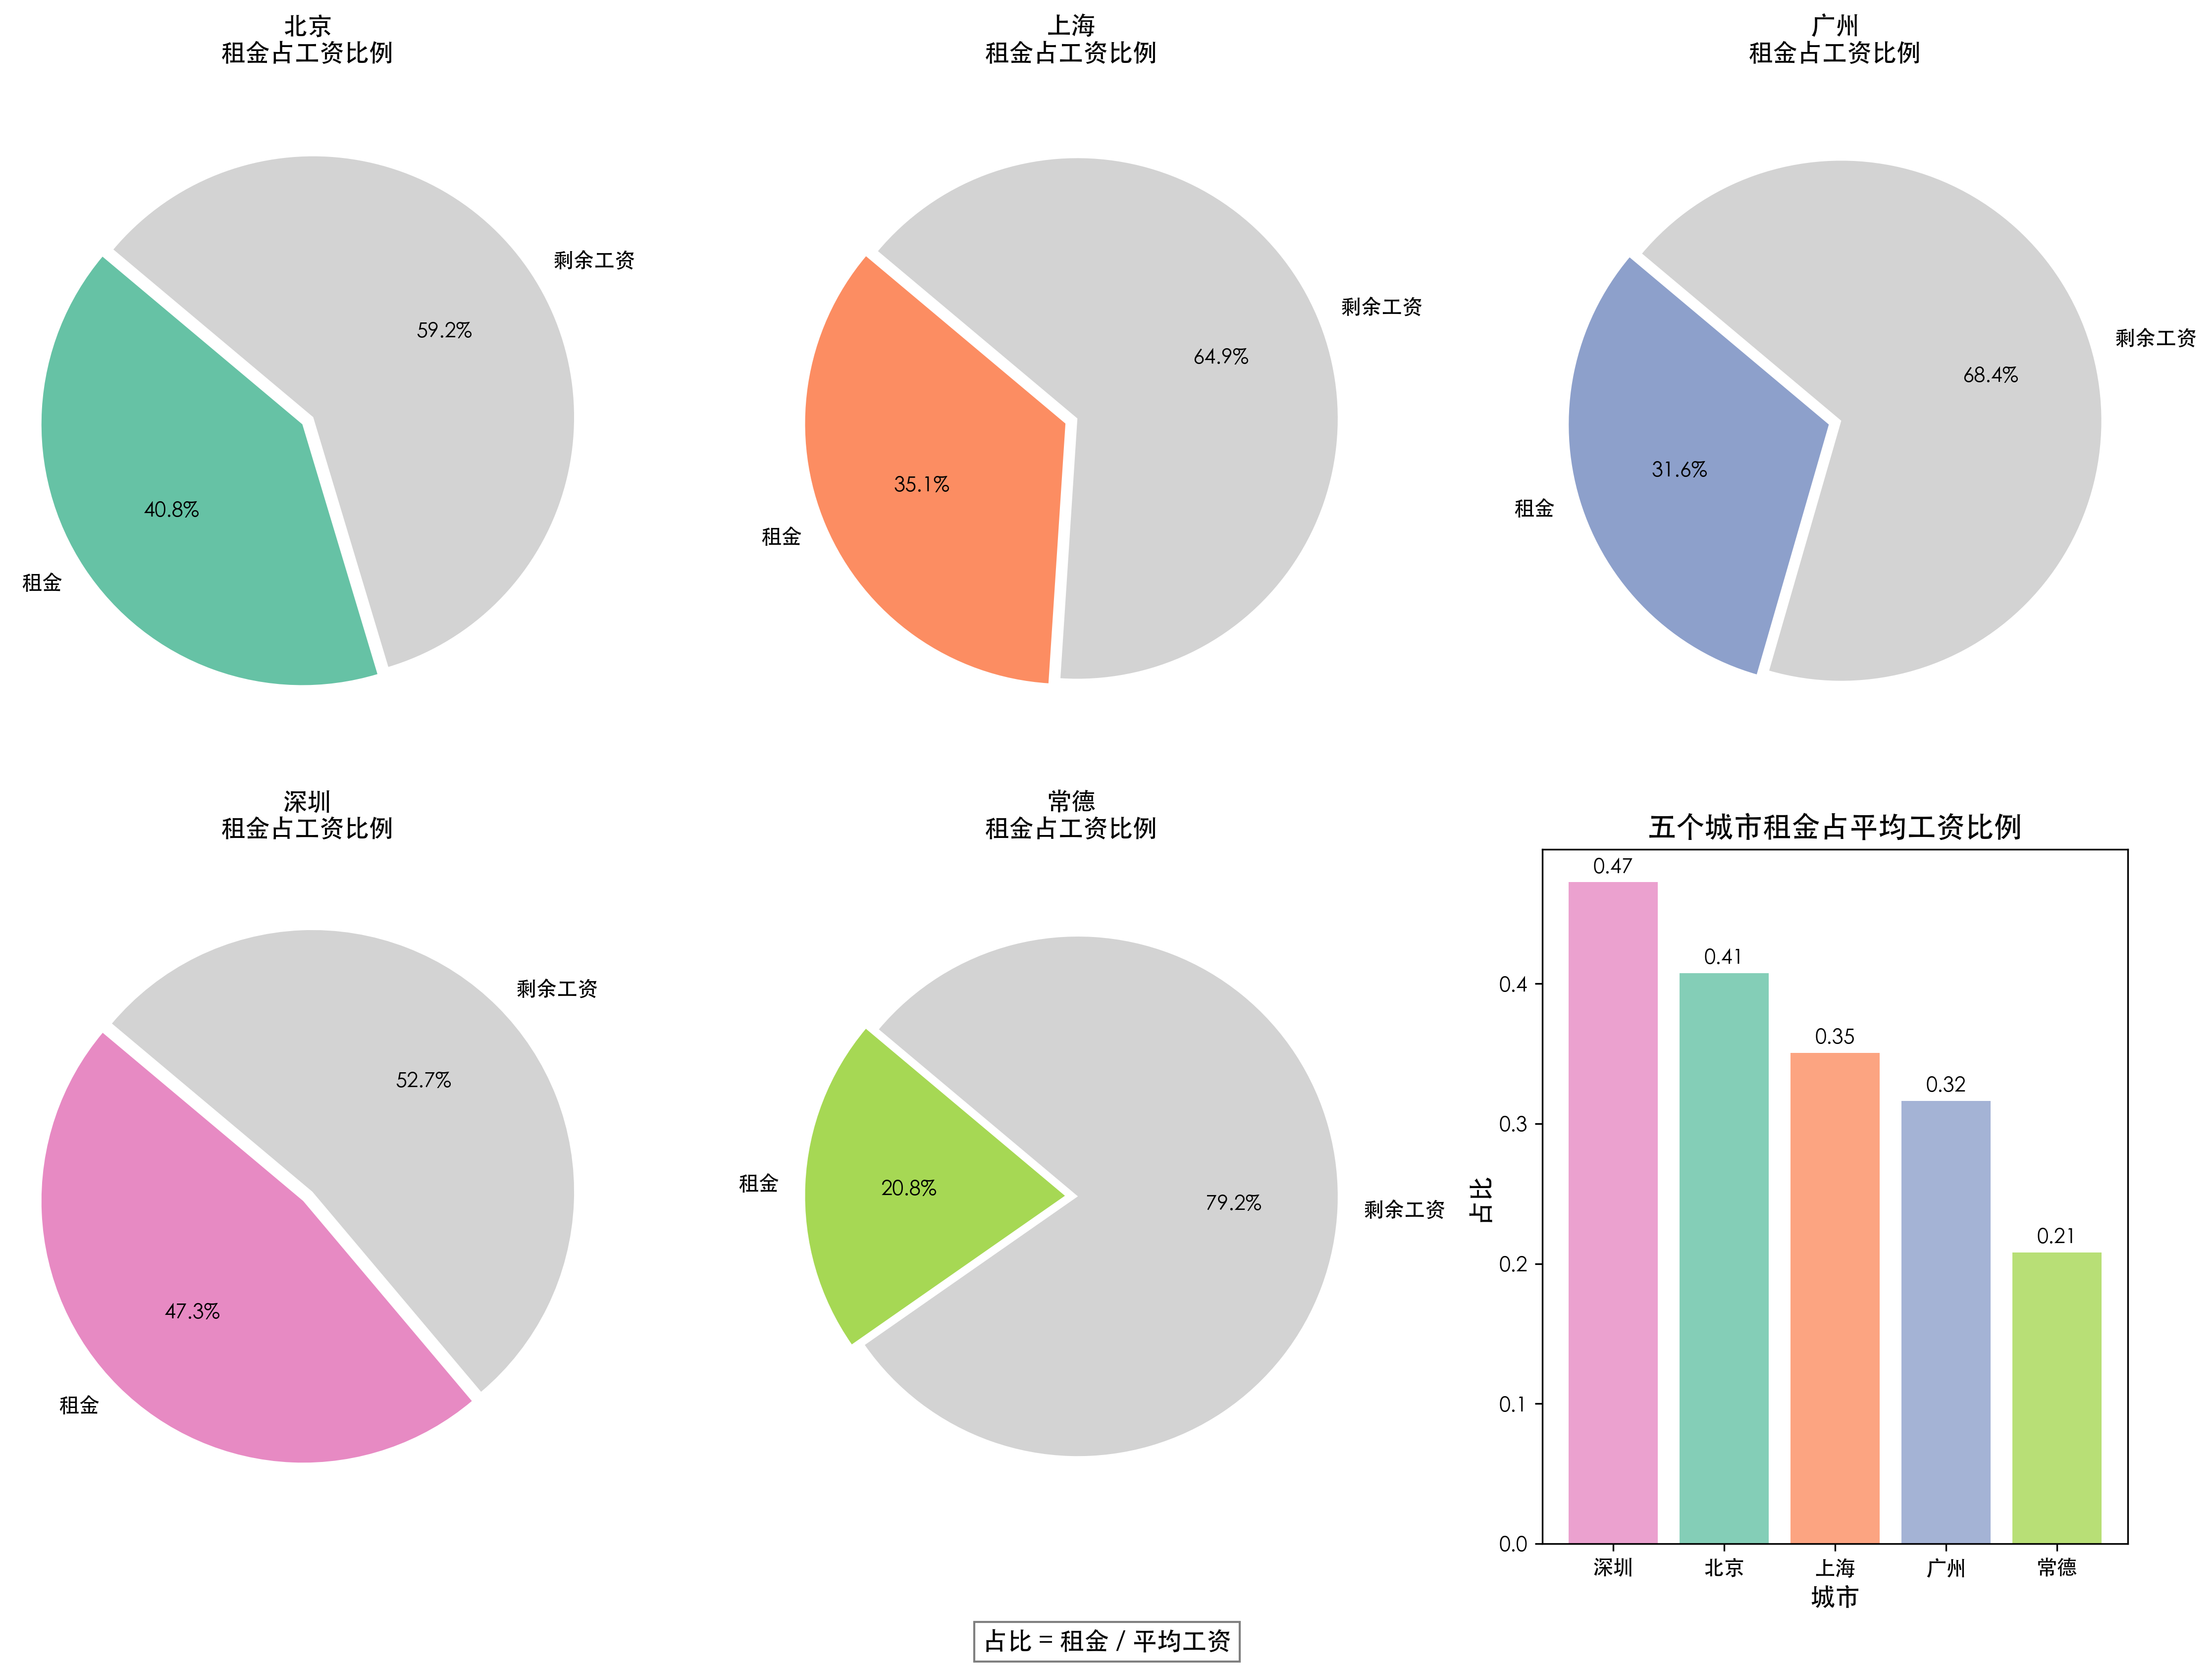
\includegraphics[width=0.7\linewidth]{../../figure/salary_price_pie_chart.png}
    \caption{五个城市租房占工资比例}
    \label{fig:salary_price_pie_chart}
\end{figure}

占比分析结果与前面的分析相同。我们可以得出结论,作为二线城市,常德的负担毫无疑问是最小的,而广州是大城市中负担相对较小者。